%
% This file is part of the GROMACS molecular simulation package.
%
% Copyright (c) 2013,2014, by the GROMACS development team, led by
% Mark Abraham, David van der Spoel, Berk Hess, and Erik Lindahl,
% and including many others, as listed in the AUTHORS file in the
% top-level source directory and at http://www.gromacs.org.
%
% GROMACS is free software; you can redistribute it and/or
% modify it under the terms of the GNU Lesser General Public License
% as published by the Free Software Foundation; either version 2.1
% of the License, or (at your option) any later version.
%
% GROMACS is distributed in the hope that it will be useful,
% but WITHOUT ANY WARRANTY; without even the implied warranty of
% MERCHANTABILITY or FITNESS FOR A PARTICULAR PURPOSE.  See the GNU
% Lesser General Public License for more details.
%
% You should have received a copy of the GNU Lesser General Public
% License along with GROMACS; if not, see
% http://www.gnu.org/licenses, or write to the Free Software Foundation,
% Inc., 51 Franklin Street, Fifth Floor, Boston, MA  02110-1301  USA.
%
% If you want to redistribute modifications to GROMACS, please
% consider that scientific software is very special. Version
% control is crucial - bugs must be traceable. We will be happy to
% consider code for inclusion in the official distribution, but
% derived work must not be called official GROMACS. Details are found
% in the README & COPYING files - if they are missing, get the
% official version at http://www.gromacs.org.
%
% To help us fund GROMACS development, we humbly ask that you cite
% the research papers on the package. Check out http://www.gromacs.org.

\chapter{Interaction function and force fields\index{force field}}
\label{ch:ff}
To accommodate the potential functions used
in some popular force fields (see \ref{sec:ff}), {\gromacs} offers a choice of functions,
both for non-bonded interaction and for dihedral interactions. They
are described in the appropriate subsections.

The potential functions can be subdivided into three parts
\begin{enumerate}
\item   {\em Non-bonded}: Lennard-Jones or Buckingham, and Coulomb or
modified Coulomb. The non-bonded interactions are computed on the
basis of a neighbor list (a list of non-bonded atoms within a certain
radius), in which exclusions are already removed.
\item   {\em Bonded}: covalent bond-stretching, angle-bending,
improper dihedrals, and proper dihedrals. These are computed on the
basis of fixed lists. 
\item   {\em Restraints}: position restraints, angle restraints,
distance restraints, orientation restraints and dihedral restraints, all
based on fixed lists. 
\end{enumerate}

\section{Non-bonded interactions}
Non-bonded interactions in {\gromacs} are pair-additive and centro-symmetric:
\beq
V(\ve{r}_1,\ldots \ve{r}_N) = \sum_{i<j}V_{ij}(\rvij);
\eeq
\beq
\ve{F}_i = -\sum_j \frac{dV_{ij}(r_{ij})}{dr_{ij}} \frac{\rvij}{r_{ij}} = -\ve{F}_j
\eeq
The non-bonded interactions contain a \normindex{repulsion} term, 
a \normindex{dispersion}
term, and a Coulomb term. The repulsion and dispersion term are
combined in either the Lennard-Jones (or 6-12 interaction), or the
Buckingham (or exp-6 potential). In addition, (partially) charged atoms
act through the Coulomb term. 

\subsection{The Lennard-Jones interaction}
\label{sec:lj}
The \normindex{Lennard-Jones} potential $V_{LJ}$ between two atoms equals:
\beq
V_{LJ}(\rij) =  \frac{C_{ij}^{(12)}}{\rij^{12}} -
                        \frac{C_{ij}^{(6)}}{\rij^6}     
\eeq
See also \figref{lj}
The parameters $C^{(12)}_{ij}$ and $C^{(6)}_{ij}$  depend on pairs of
{\em atom types}; consequently they are taken from a matrix of
LJ-parameters. In the Verlet cut-off scheme, the potential is shifted
by a constant such that it is zero at the cut-off distance.

\begin{figure}
\centerline{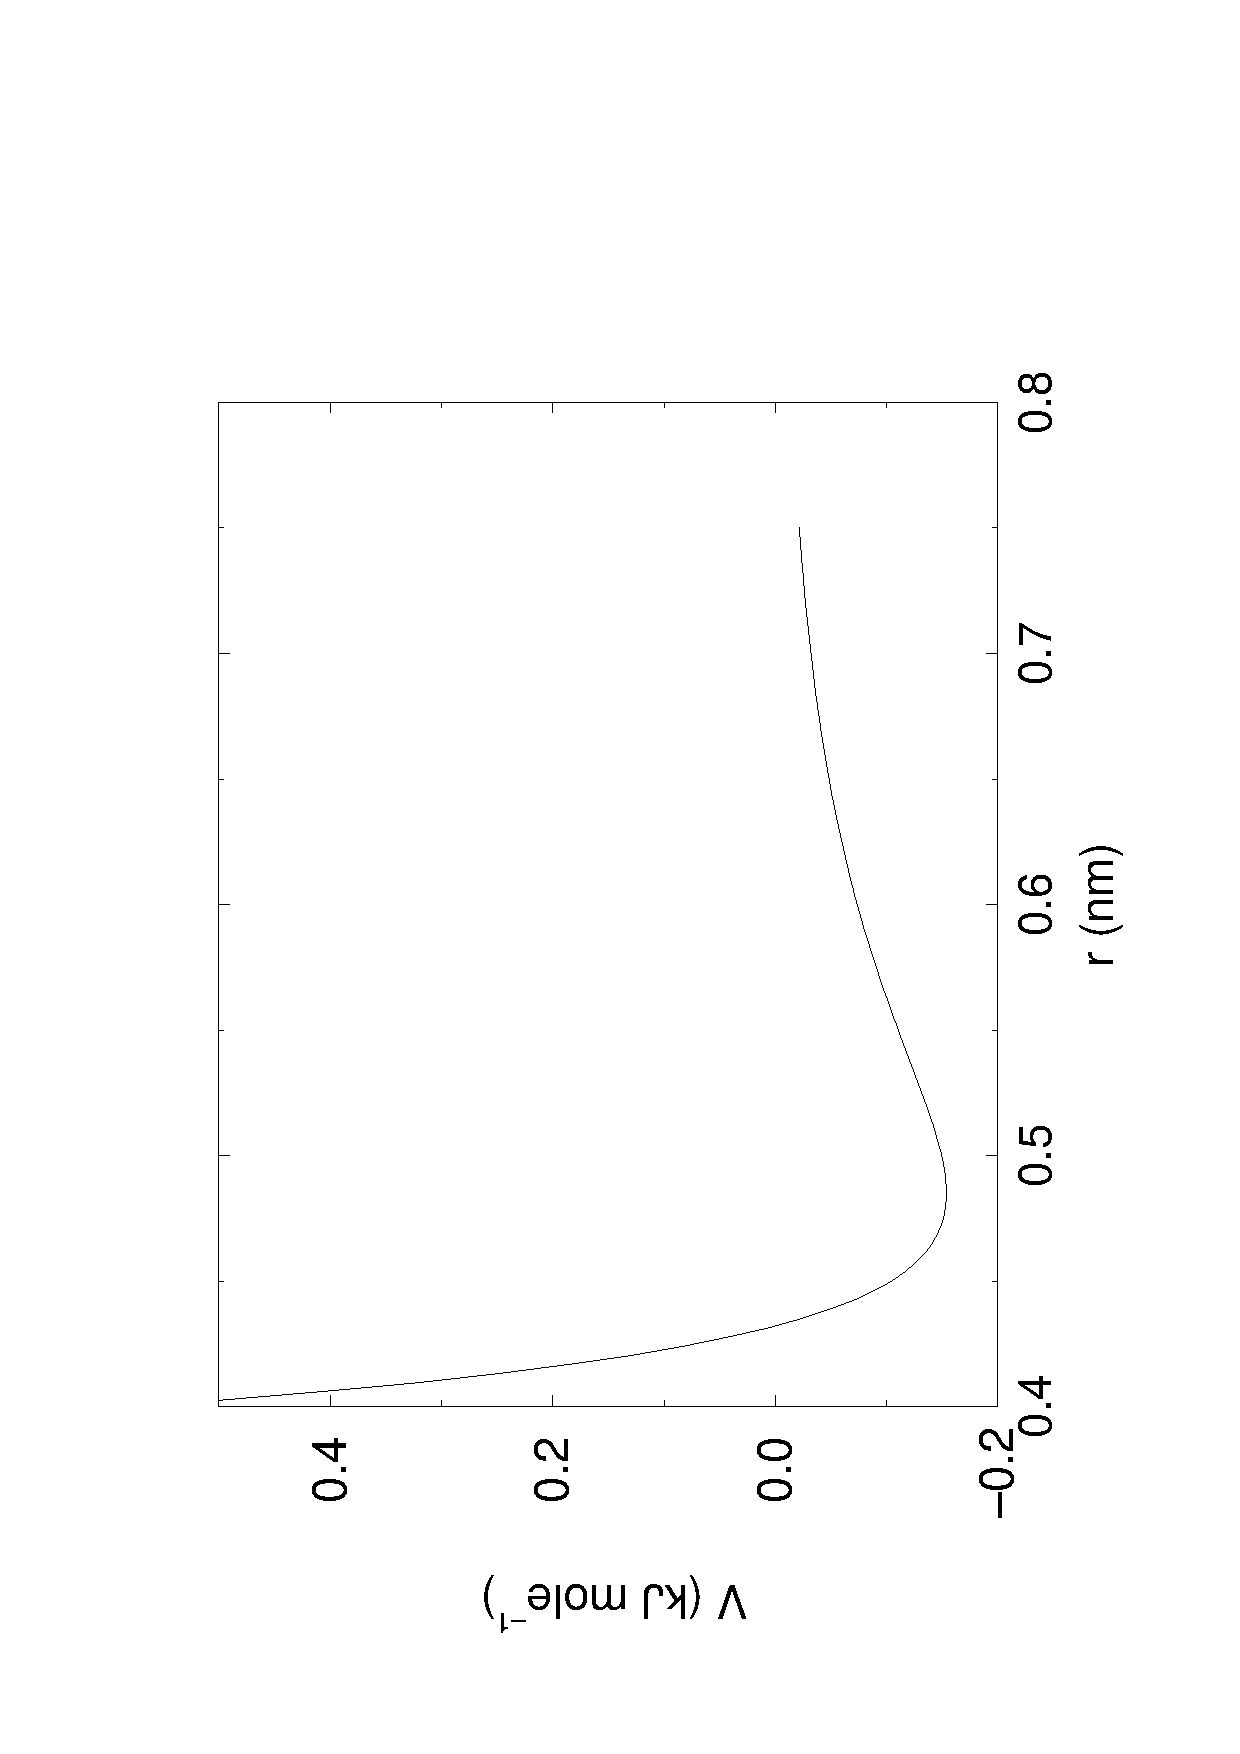
\includegraphics[width=8cm]{plots/f-lj}}
\caption {The Lennard-Jones interaction.}
\label{fig:lj}
\end{figure}
 
The force derived from this potential is:
\beq
\ve{F}_i(\rvij) = \left( 12~\frac{C_{ij}^{(12)}}{\rij^{13}} -
                                 6~\frac{C_{ij}^{(6)}}{\rij^7} \right) \rnorm 
\eeq

The LJ potential may also be written in the following form:
\beq
V_{LJ}(\rvij) = 4\epsilon_{ij}\left(\left(\frac{\sigma_{ij}} {\rij}\right)^{12}
                - \left(\frac{\sigma_{ij}}{\rij}\right)^{6} \right)
\label{eqn:sigeps}      
\eeq

In constructing the parameter matrix for the non-bonded LJ-parameters,
two types of \normindex{combination rule}s can be used within {\gromacs},
only geometric averages (type 1 in the input section of the force-field file):
\beq
\begin{array}{rcl}
C_{ij}^{(6)}    &=& \left({C_{ii}^{(6)} \, C_{jj}^{(6)}}\right)^{1/2}    \\
C_{ij}^{(12)}   &=& \left({C_{ii}^{(12)} \, C_{jj}^{(12)}}\right)^{1/2}
\label{eqn:comb}
\end{array}
\eeq
or, alternatively the Lorentz-Berthelot rules can be used. An arithmetic average is used to calculate $\sigma_{ij}$, while a geometric average is used to calculate $\epsilon_{ij}$ (type 2):
\beq
\begin{array}{rcl}
 \sigma_{ij}   &=& \frac{1}{ 2}(\sigma_{ii} + \sigma_{jj})        \\
 \epsilon_{ij} &=& \left({\epsilon_{ii} \, \epsilon_{jj}}\right)^{1/2}
 \label{eqn:lorentzberthelot}
\end{array}
\eeq
finally an geometric average for both parameters can be used (type 3):
\beq
\begin{array}{rcl}
 \sigma_{ij}   &=& \left({\sigma_{ii} \, \sigma_{jj}}\right)^{1/2}        \\
 \epsilon_{ij} &=& \left({\epsilon_{ii} \, \epsilon_{jj}}\right)^{1/2}
\end{array}
\eeq
This last rule is used by the OPLS force field.


%\ifthenelse{\equal{\gmxlite}{1}}{}{
\subsection{\normindex{Buckingham potential}}
The Buckingham
potential has a more flexible and realistic repulsion term
than the Lennard-Jones interaction, but is also more expensive to
compute. The potential form is:
\beq
V_{bh}(\rij) = A_{ij} \exp(-B_{ij} \rij) -
                        \frac{C_{ij}}{\rij^6}
\eeq
\begin{figure}
\centerline{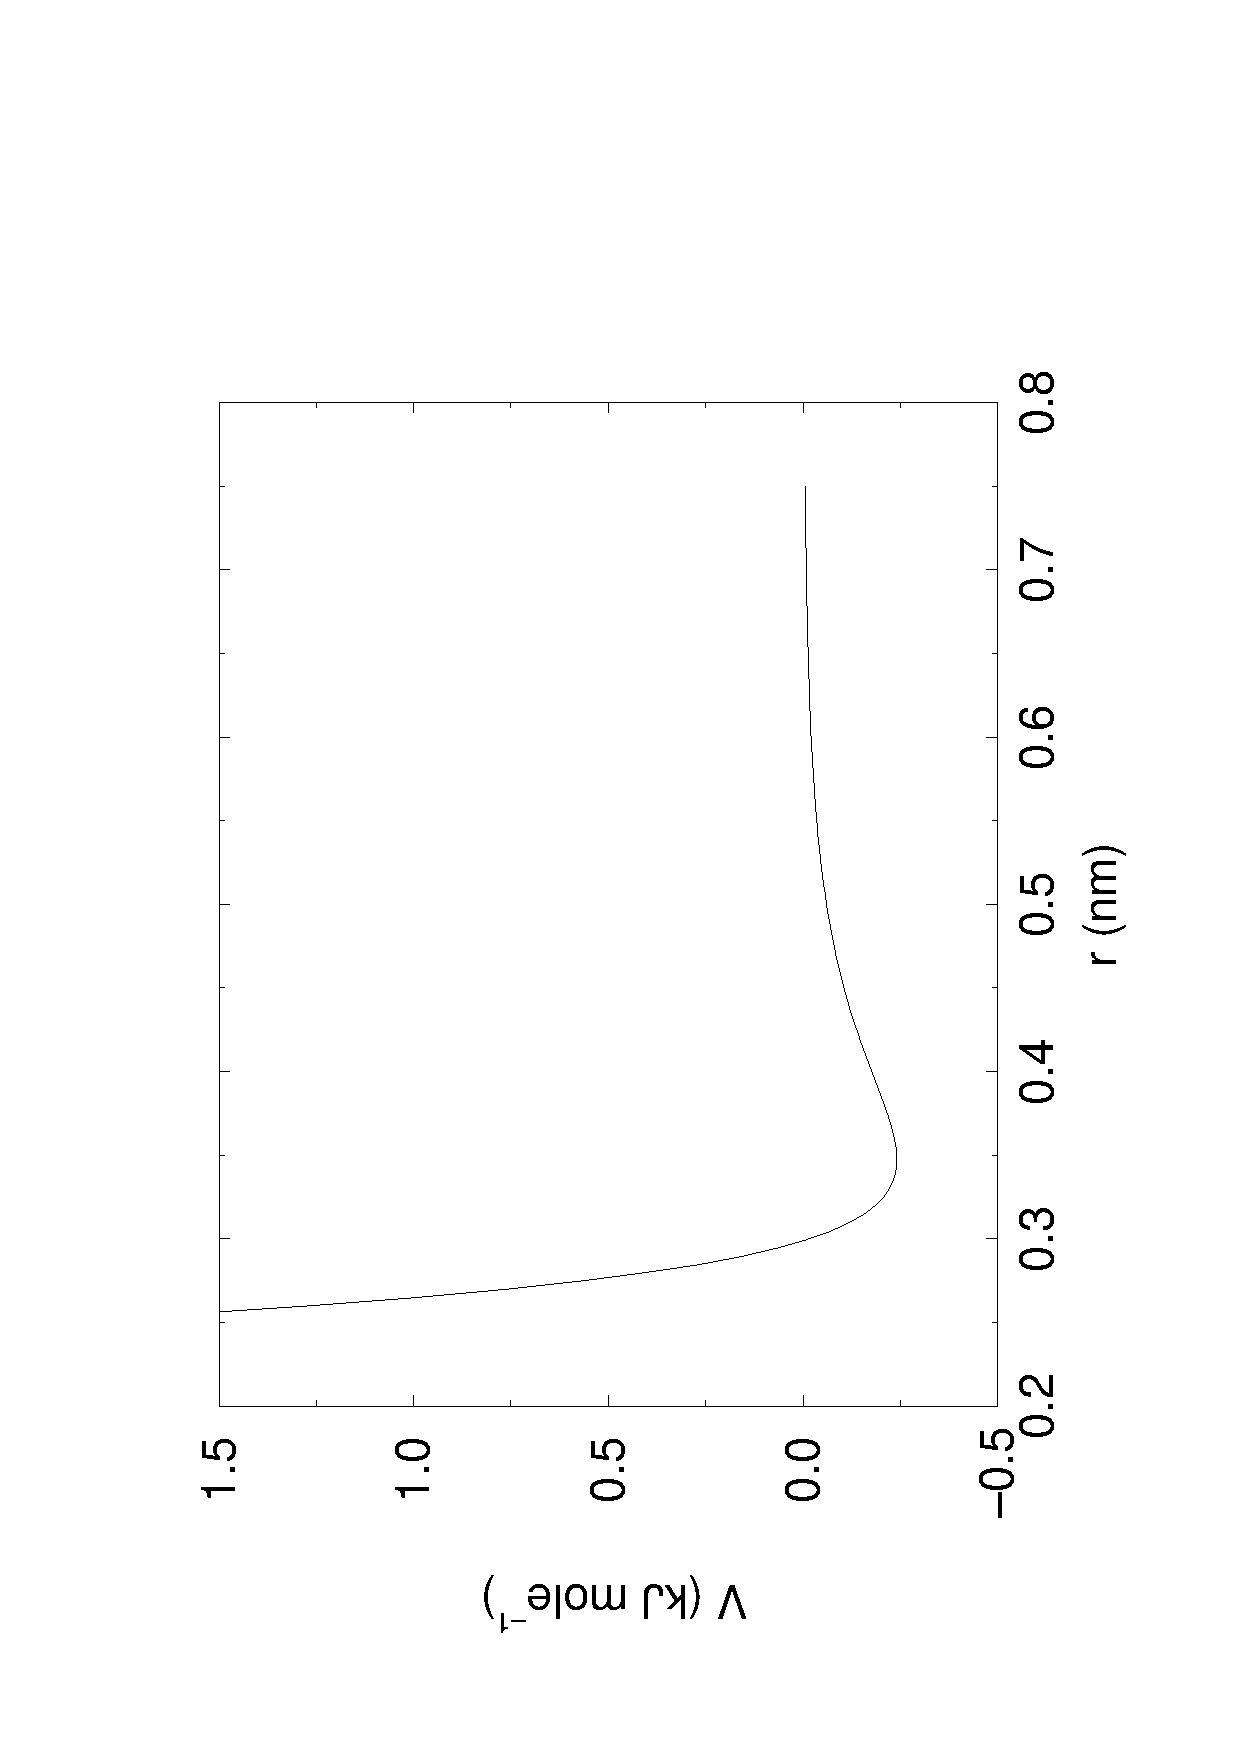
\includegraphics[width=8cm]{plots/f-bham}}
\caption {The Buckingham interaction.}
\label{fig:bham}
\end{figure}

See also \figref{bham}.  The force derived from this is:
\beq
 \ve{F}_i(\rij) = \left[ A_{ij}B_{ij}\exp(-B_{ij} \rij) -
                                 6\frac{C_{ij}}{\rij^7} \right] \rnorm
\eeq

%} % Brace matches ifthenelse test for gmxlite

\subsection{Coulomb interaction}
\label{sec:coul}
\newcommand{\epsr}{\varepsilon_r}
\newcommand{\epsrf}{\varepsilon_{rf}}
The \normindex{Coulomb} interaction between two charge particles is given by:
\beq
V_c(\rij) = f \frac{q_i q_j}{\epsr \rij}
\label{eqn:vcoul}
\eeq
See also \figref{coul}, where $f = \frac{1}{4\pi \varepsilon_0} =
138.935\,485$ (see \chref{defunits})

\begin{figure}
\centerline{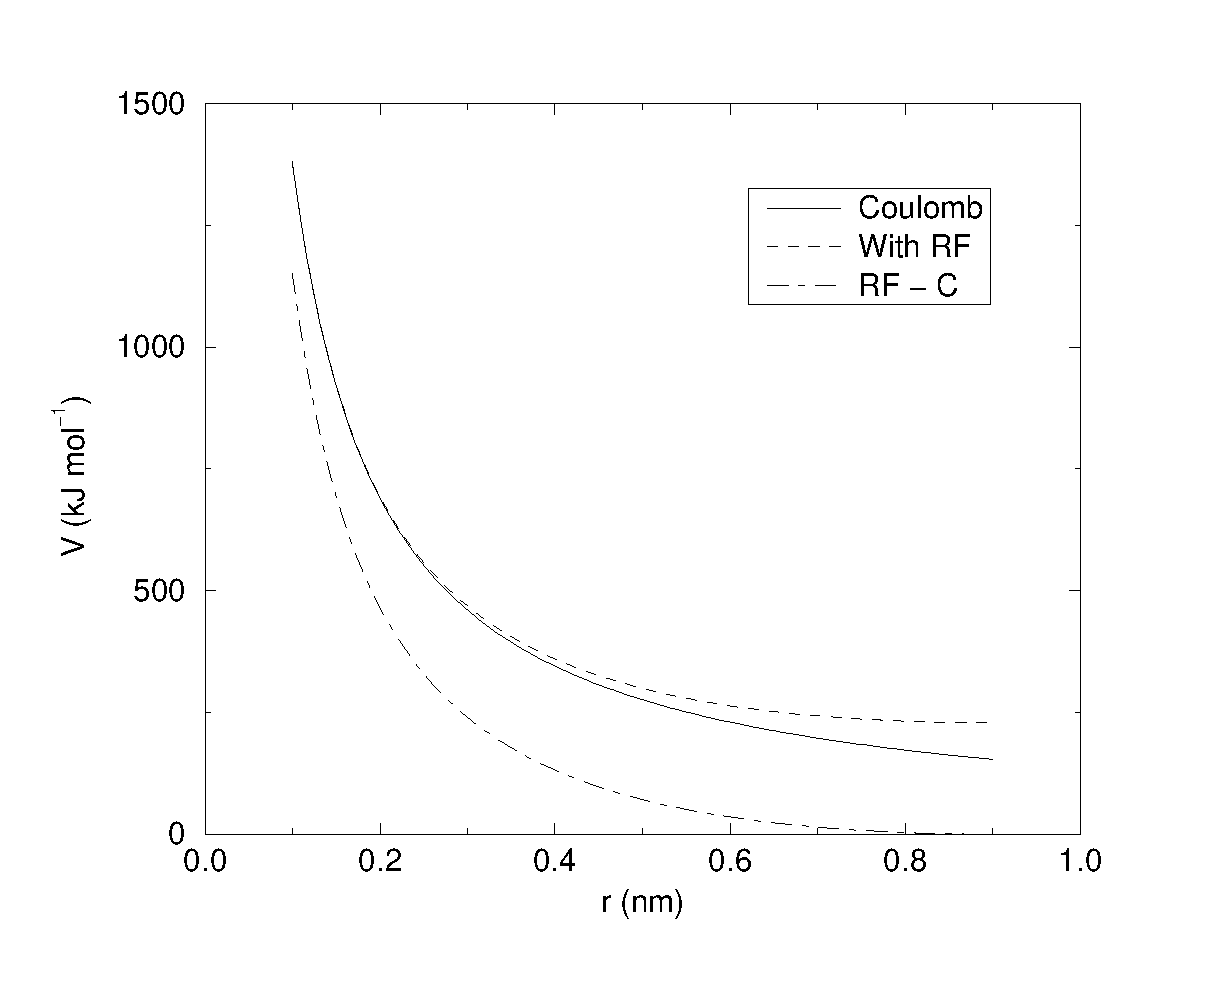
\includegraphics[width=8cm]{plots/vcrf}}
\caption[The Coulomb interaction with and without reaction field.]{The
Coulomb interaction (for particles with equal signed charge) with and
without reaction field. In the latter case $\epsr$ was 1, $\epsrf$ was 78,
and $r_c$ was 0.9 nm.
The dot-dashed line is the same as the dashed line, except for a constant.}
\label{fig:coul}
\end{figure}

The force derived from this potential is:
\beq
\ve{F}_i(\rvij) = f \frac{q_i q_j}{\epsr\rij^2}\rnorm
\eeq

A plain Coulomb interaction should only be used without cut-off or when all pairs fall within the cut-off, since there is an abrupt, large change in the force at the cut-off. In case you do want to use a cut-off, the potential can be shifted by a constant to make the potential the integral of the force. With the group cut-off scheme, this shift is only applied to non-excluded pairs. With the Verlet cut-off scheme, the shift is also applied to excluded pairs and self interactions, which makes the potential equivalent to a reaction field with $\epsrf=1$ (see below).

In {\gromacs} the  relative \swapindex{dielectric}{constant} 
\normindex{$\epsr$}
may be set in the in the input for {\tt grompp}. 

%\ifthenelse{\equal{\gmxlite}{1}}{}{
\subsection{Coulomb interaction with \normindex{reaction field}}
\label{sec:coulrf}
The Coulomb interaction can be modified for homogeneous systems by
assuming a constant dielectric environment beyond the cut-off $r_c$
with a dielectric constant of {$\epsrf$}. The interaction then reads:
\beq
V_{crf} ~=~
  f \frac{q_i q_j}{\epsr\rij}\left[1+\frac{\epsrf-\epsr}{2\epsrf+\epsr}
  \,\frac{\rij^3}{r_c^3}\right]
  - f\frac{q_i q_j}{\epsr r_c}\,\frac{3\epsrf}{2\epsrf+\epsr}
\label{eqn:vcrf}
\eeq
in which the constant expression on the right makes the potential
zero at the cut-off $r_c$. For charged cut-off spheres this corresponds
to neutralization with a homogeneous background charge.
We can rewrite \eqnref{vcrf} for simplicity as
\beq
V_{crf} ~=~     f \frac{q_i q_j}{\epsr}\left[\frac{1}{\rij} + k_{rf}~ \rij^2 -c_{rf}\right]
\eeq
with
\bea
k_{rf}  &=&     \frac{1}{r_c^3}\,\frac{\epsrf-\epsr}{(2\epsrf+\epsr)}   \label{eqn:krf}\\
c_{rf}  &=&     \frac{1}{r_c}+k_{rf}\,r_c^2 ~=~ \frac{1}{r_c}\,\frac{3\epsrf}{(2\epsrf+\epsr)}
\label{eqn:crf}
\eea
For large $\epsrf$ the $k_{rf}$ goes to $r_c^{-3}/2$,
while for $\epsrf$ = $\epsr$ the correction vanishes.
In \figref{coul}
the modified interaction is plotted, and it is clear that the derivative 
with respect to $\rij$ (= -force) goes to zero at the cut-off distance.
The force derived from this potential reads:
\beq
\ve{F}_i(\rvij) = f \frac{q_i q_j}{\epsr}\left[\frac{1}{\rij^2} - 2 k_{rf}\rij\right]\rnorm
\label{eqn:fcrf}
\eeq
The reaction-field correction should also be applied to all excluded
atoms pairs, including self pairs, in which case the normal Coulomb
term in \eqnsref{vcrf}{fcrf} is absent.

Tironi {\etal} have introduced a generalized reaction field in which
the dielectric continuum beyond the cut-off $r_c$ also has an ionic strength
$I$~\cite{Tironi95}. In this case we can rewrite the constants $k_{rf}$ and 
$c_{rf}$ using the inverse Debye screening length $\kappa$:
\bea
\kappa^2  &=&     
   \frac{2 I \,F^2}{\varepsilon_0 \epsrf RT}
   = \frac{F^2}{\varepsilon_0 \epsrf RT}\sum_{i=1}^{K} c_i z_i^2     \\
k_{rf}  &=&     \frac{1}{r_c^3}\,
    \frac{(\epsrf-\epsr)(1 + \kappa r_c) + \half\epsrf(\kappa r_c)^2}
         {(2\epsrf + \epsr)(1 + \kappa r_c) + \epsrf(\kappa r_c)^2}
    \label{eqn:kgrf}\\
c_{rf}  &=&     \frac{1}{r_c}\,
    \frac{3\epsrf(1 + \kappa r_c + \half(\kappa r_c)^2)}
         {(2\epsrf+\epsr)(1 + \kappa r_c) + \epsrf(\kappa r_c)^2}
    \label{eqn:cgrf}
\eea
where $F$ is Faraday's constant, $R$ is the ideal gas constant, $T$
the absolute temperature, $c_i$ the molar concentration for species
$i$ and $z_i$ the charge number of species $i$ where we have $K$
different species. In the limit of zero ionic strength ($\kappa=0$)
\eqnsref{kgrf}{cgrf} reduce to the simple forms of \eqnsref{krf}{crf}
respectively.

\subsection{Modified non-bonded interactions}
\label{sec:mod_nb_int}
In {\gromacs}, the non-bonded potentials can be
modified by a shift function. The purpose of this is to replace the
truncated forces by forces that are continuous and have continuous
derivatives at the \normindex{cut-off} radius. With such forces the
timestep integration produces much smaller errors and there are no
such complications as creating charges from dipoles by the truncation
procedure. In fact, by using shifted forces there is no need for
charge groups in the construction of neighbor lists. However, the
shift function produces a considerable modification of the Coulomb
potential. Unless the ``missing'' long-range potential is properly
calculated and added (through the use of PPPM, Ewald, or PME), the
effect of such modifications must be carefully evaluated.  The
modification of the Lennard-Jones dispersion and repulsion is only
minor, but it does remove the noise caused by cut-off effects.
 
There is {\em no} fundamental difference between a switch function
(which multiplies the potential with a function) and a shift function
(which adds a function to the force or potential)~\cite{Spoel2006a}. The switch
function is a special case of the shift function, which we apply to
the {\em force function} $F(r)$, related to the electrostatic or
van der Waals force acting on particle $i$ by particle $j$ as:
\beq
\ve{F}_i = c F(r_{ij}) \frac{\rvij}{r_{ij}}
\eeq
For pure Coulomb or Lennard-Jones interactions
$F(r)=F_\alpha(r)=r^{-(\alpha+1)}$.
The shifted force $F_s(r)$ can generally be written as:
\beq
\begin{array}{rcl}
\vspace{2mm}
F_s(r)~=&~F_\alpha(r)   & r < r_1               \\
\vspace{2mm}
F_s(r)~=&~F_\alpha(r)+S(r)      & r_1 \le r < r_c       \\
F_s(r)~=&~0             & r_c \le r     
\end{array}
\eeq
When $r_1=0$ this is a traditional shift function, otherwise it acts as a 
switch function. The corresponding shifted coulomb potential then reads:
\beq
V_s(r_{ij}) = f \Phi_s (r_{ij}) q_i q_j
\eeq
where $\Phi(r)$ is the potential function 
\beq
\Phi_s(r) =  \int^{\infty}_r~F_s(x)\, dx
\eeq

The {\gromacs} shift function should be smooth at the boundaries, therefore
the following boundary conditions are imposed on the shift function:
\beq
\begin{array}{rcl}
S(r_1)          &=&0            \\
S'(r_1)         &=&0            \\
S(r_c)          &=&-F_\alpha(r_c)       \\
S'(r_c)         &=&-F_\alpha'(r_c)
\end{array}
\eeq
A 3$^{rd}$ degree polynomial of the form
\beq
S(r) = A(r-r_1)^2 + B(r-r_1)^3
\eeq
fulfills these requirements. The constants A and B are given by the
boundary condition at $r_c$: 
\beq
\begin{array}{rcl}
\vspace{2mm}
A &~=~& -\displaystyle
        \frac{(\alpha+4)r_c~-~(\alpha+1)r_1} {r_c^{\alpha+2}~(r_c-r_1)^2} \\
B &~=~& \displaystyle
        \frac{(\alpha+3)r_c~-~(\alpha+1)r_1}{r_c^{\alpha+2}~(r_c-r_1)^3}
\end{array}
\eeq
Thus the total force function is:
\beq
F_s(r) = \frac{\alpha}{r^{\alpha+1}} + A(r-r_1)^2 + B(r-r_1)^3
\eeq
and the potential function reads:
\beq
\Phi(r) = \frac{1}{r^\alpha} - \frac{A}{3} (r-r_1)^3 - \frac{B}{4} (r-r_1)^4 - C
\eeq
where 
\beq
C =  \frac{1}{r_c^\alpha} - \frac{A}{3} (r_c-r_1)^3 - \frac{B}{4} (r_c-r_1)^4
\eeq

When $r_1$ = 0, the modified Coulomb force function is
\beq
 F_s(r) = \frac{1}{r^2} - \frac{5 r^2}{r_c^4} + \frac{4 r^3}{r_c^5}
\eeq
which is identical to the {\em \index{parabolic force}} 
function recommended to be used as a short-range function in 
conjunction with a \swapindex{Poisson}{solver} 
for the long-range part~\cite{Berendsen93a}.
The modified Coulomb potential function is:
\beq
\Phi(r) = \frac{1}{r} - \frac{5}{3r_c} + \frac{5r^3}{3r_c^4} - \frac{r^4}{r_c^5}
\eeq
See also \figref{shift}.

\begin{figure}
\centerline{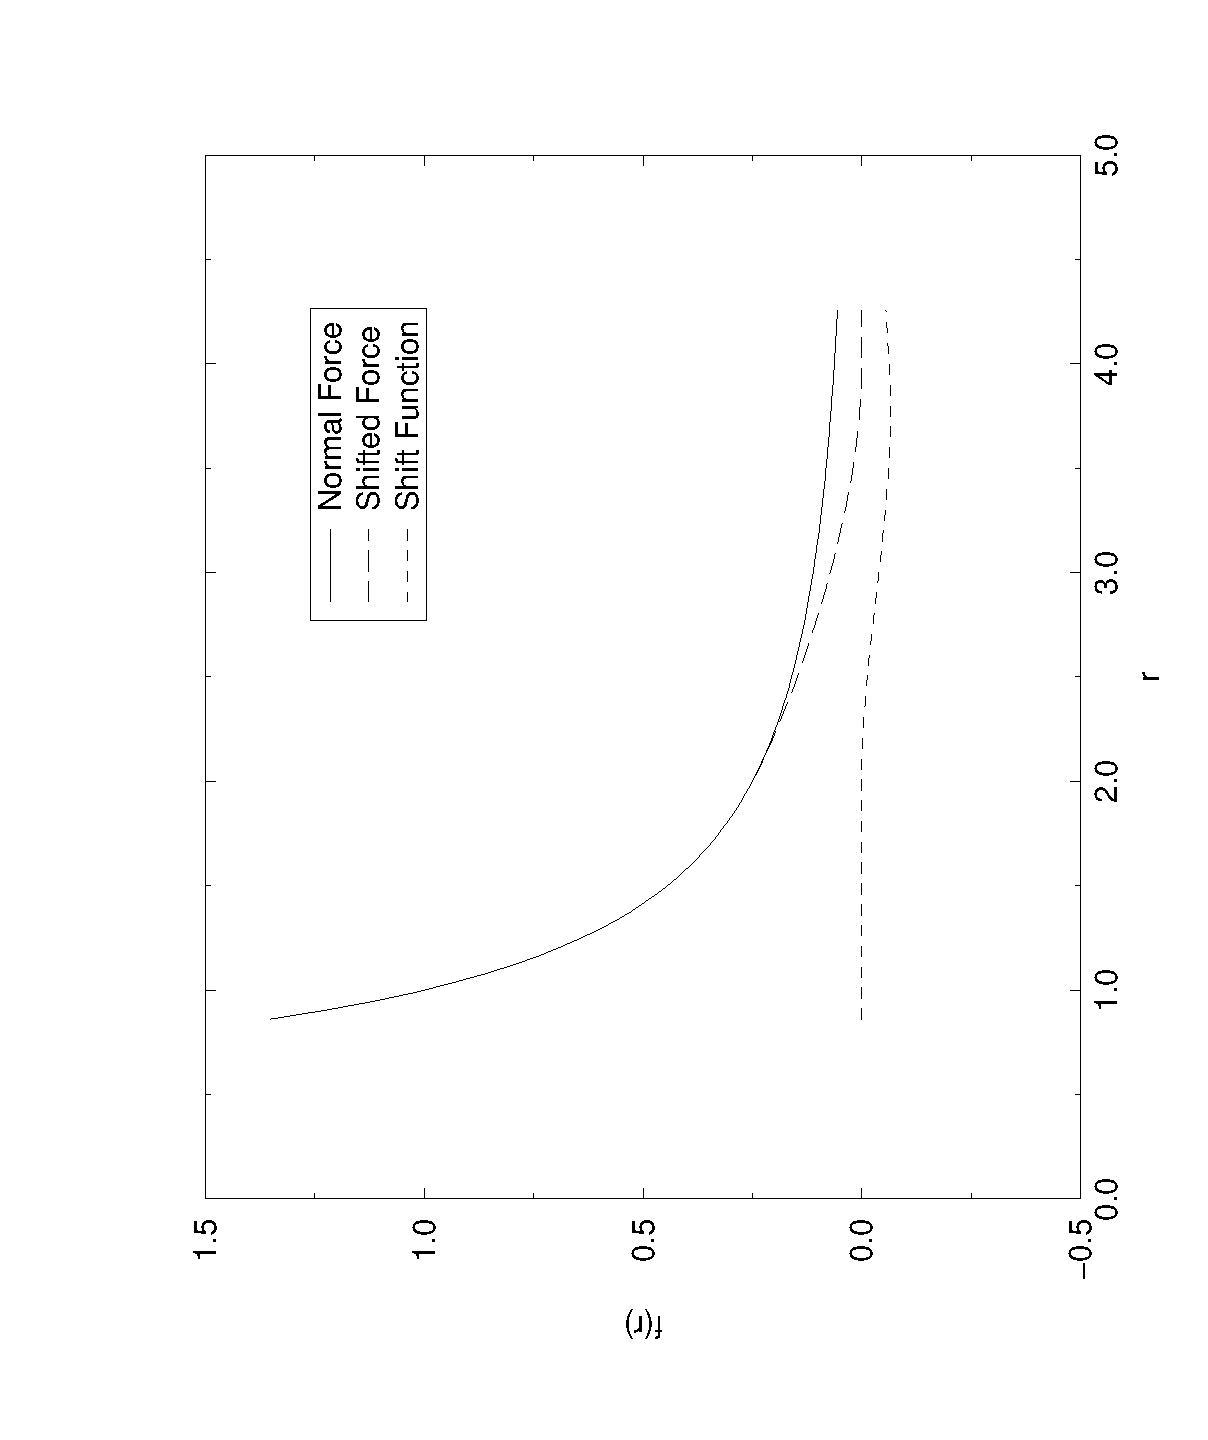
\includegraphics[width=10cm]{plots/shiftf}}
\caption[The Coulomb Force, Shifted Force and Shift Function
$S(r)$,.]{The Coulomb Force, Shifted Force and Shift Function $S(r)$,
using r$_1$ = 2 and r$_c$ = 4.} 
\label{fig:shift}
\end{figure}

\subsection{Modified short-range interactions with Ewald summation}
When Ewald summation\index{Ewald sum} or \seeindex{particle-mesh
Ewald}{PME}\index{Ewald, particle-mesh} is used to calculate the
long-range interactions, the 
short-range Coulomb potential must also be modified, similar to the
switch function above. In this case the short range potential is given
by:
\beq
V(r) = f \frac{\mbox{erfc}(\beta r_{ij})}{r_{ij}} q_i q_j,
\eeq
where $\beta$ is a parameter that determines the relative weight 
between the direct space sum and the reciprocal space sum and erfc$(x)$ is
the complementary error function. For further 
details on long-range electrostatics, see \secref{lr_elstat}.
%} % Brace matches ifthenelse test for gmxlite


\section{Bonded interactions}
Bonded interactions are based on a fixed list of atoms. They are not
exclusively pair interactions, but include 3- and 4-body interactions
as well. There are {\em bond stretching} (2-body), {\em bond angle}
(3-body), and {\em dihedral angle} (4-body) interactions. A special
type of dihedral interaction (called {\em improper dihedral}) is used
to force atoms to remain in a plane or to prevent transition to a
configuration of opposite chirality (a mirror image).

\subsection{Bond stretching}
\label{sec:bondpot}
\subsubsection{Harmonic potential}
\label{subsec:harmonicbond}
The \swapindex{bond}{stretching} between two covalently bonded atoms
$i$ and $j$ is represented by a harmonic potential:

\begin{figure}
\centerline{\raisebox{2cm}{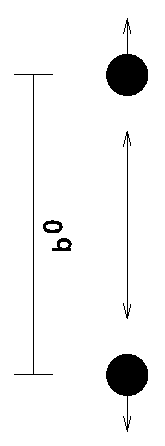
\includegraphics[width=5cm]{plots/bstretch}}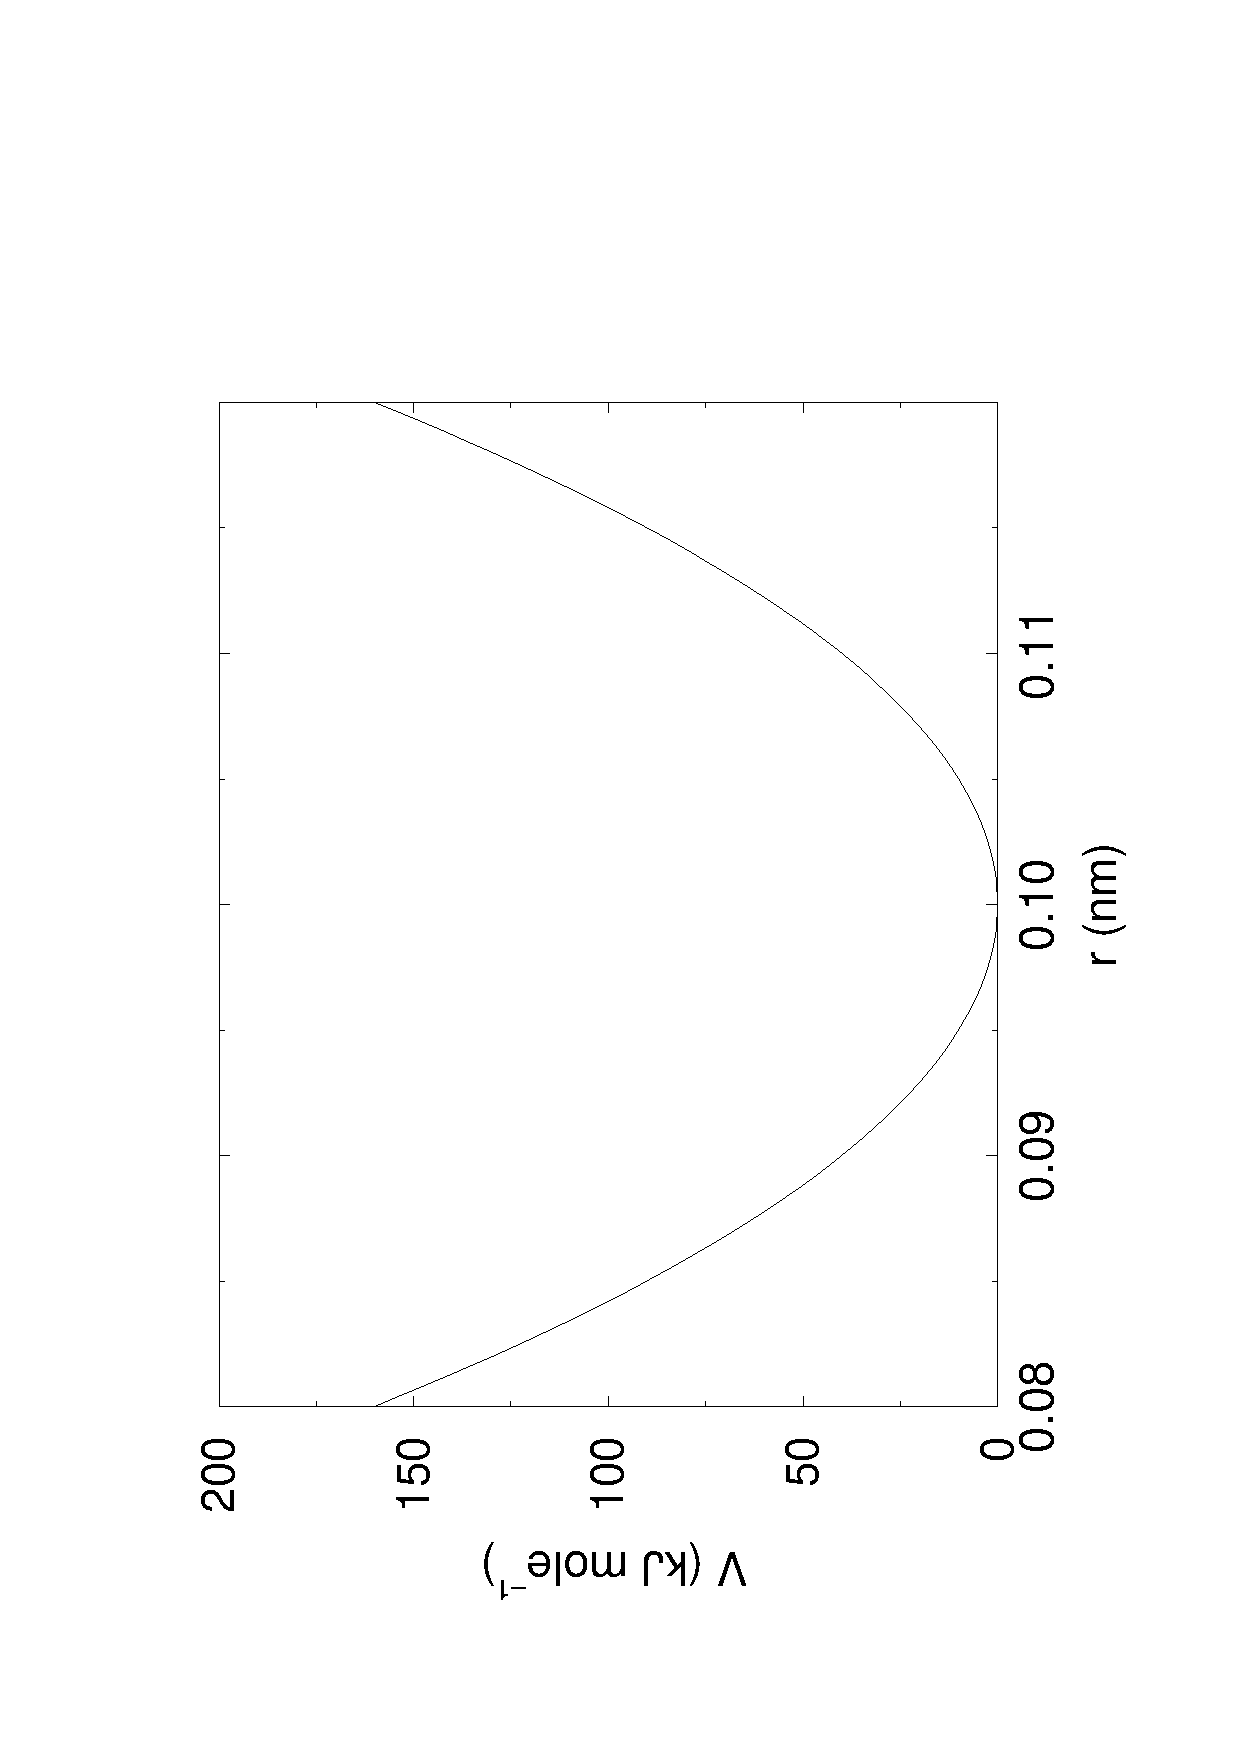
\includegraphics[width=7cm]{plots/f-bond}}
\caption[Bond stretching.]{Principle of bond stretching (left), and the bond
stretching potential (right).}
\label{fig:bstretch1}
\end{figure}

\beq
V_b~(\rij) = \half k^b_{ij}(\rij-b_{ij})^2
\eeq
See also \figref{bstretch1}, with the force given by:
\beq
\ve{F}_i(\rvij) = k^b_{ij}(\rij-b_{ij}) \rnorm
\eeq

%\ifthenelse{\equal{\gmxlite}{1}}{}{
\subsubsection{Fourth power potential}
\label{subsec:G96bond}
In the \gromosv{96} force field~\cite{gromos96}, the covalent bond potential
is, for reasons of computational efficiency, written as:
\beq
V_b~(\rij) = \frac{1}{4}k^b_{ij}\left(\rij^2-b_{ij}^2\right)^2
\eeq
The corresponding force is:
\beq
\ve{F}_i(\rvij) = k^b_{ij}(\rij^2-b_{ij}^2)~\rvij
\eeq
The force constants for this form of the potential are related to the usual
harmonic force constant $k^{b,\mathrm{harm}}$ (\secref{bondpot}) as
\beq
2 k^b b_{ij}^2 = k^{b,\mathrm{harm}}
\eeq
The force constants are mostly derived from the harmonic ones used in 
\gromosv{87}~\cite{biomos}. Although this form is computationally more 
efficient
(because no square root has to be evaluated), it is conceptually more
complex. One particular disadvantage is that since the form is not harmonic,
the average energy of a single bond is not equal to $\half kT$ as it is for 
the normal harmonic potential.

\subsection{\normindex{Morse potential} bond stretching}
\label{subsec:Morsebond}
%\author{F.P.X. Everdij}
%
For some systems that require an anharmonic bond stretching potential,
the Morse potential~\cite{Morse29} 
between two atoms {\it i} and {\it j} is available
in {\gromacs}. This potential differs from the harmonic potential in 
that it has an asymmetric potential well and a zero force at infinite
distance. The functional form is:
\beq
\displaystyle V_{morse} (r_{ij}) = D_{ij} [1 - \exp(-\beta_{ij}(r_{ij}-b_{ij}))]^2,
\eeq
See also \figref{morse}, and the corresponding force is:
\beq
\begin{array}{rcl}
\displaystyle {\bf F}_{morse} ({\bf r}_{ij})&=&2 D_{ij} \beta_{ij} r_{ij} \exp(-\beta_{ij}(r_{ij}-b_{ij})) * \\
\displaystyle \: & \: &[1 - \exp(-\beta_{ij}(r_{ij}-b_{ij}))] \frac{\displaystyle {\bf r}_{ij}}{\displaystyle r_{ij}},
\end{array}
\eeq
where \( \displaystyle D_{ij} \) is the depth of the well in kJ/mol,
\( \displaystyle \beta_{ij} \) defines the steepness of the well (in
nm\(^{-1} \)), and \( \displaystyle b_{ij} \) is the equilibrium
distance in nm.  The steepness parameter \( \displaystyle \beta_{ij}
\) can be expressed in terms of the reduced mass of the atoms {\it i}
and {\it j}, the fundamental vibration frequency \( \displaystyle
\omega_{ij} \) and the well depth \( \displaystyle D_{ij} \):
\beq
\displaystyle \beta_{ij}= \omega_{ij} \sqrt{\frac{\mu_{ij}}{2 D_{ij}}}
\eeq
and because \( \displaystyle \omega = \sqrt{k/\mu} \), one can rewrite \( \displaystyle \beta_{ij} \) in terms of the harmonic force constant \( \displaystyle k_{ij} \):
\beq
\displaystyle \beta_{ij}= \sqrt{\frac{k_{ij}}{2 D_{ij}}}
\label{eqn:betaij}
\eeq
For small deviations \( \displaystyle (r_{ij}-b_{ij}) \), one can
approximate the \( \displaystyle \exp \)-term to first-order using a
Taylor expansion:
\beq
\displaystyle \exp(-x) \approx 1-x
\label{eqn:expminx}
\eeq
and substituting \eqnref{betaij} and \eqnref{expminx} in the functional form:
\beq
\begin{array}{rcl}
\displaystyle V_{morse} (r_{ij})&=&D_{ij} [1 - \exp(-\beta_{ij}(r_{ij}-b_{ij}))]^2\\
\displaystyle \:&=&D_{ij} [1 - (1 -\sqrt{\frac{k_{ij}}{2 D_{ij}}}(r_{ij}-b_{ij}))]^2\\
\displaystyle \:&=&\frac{1}{2} k_{ij} (r_{ij}-b_{ij}))^2
\end{array}
\eeq
we recover the harmonic bond stretching potential.

\begin{figure}
\centerline{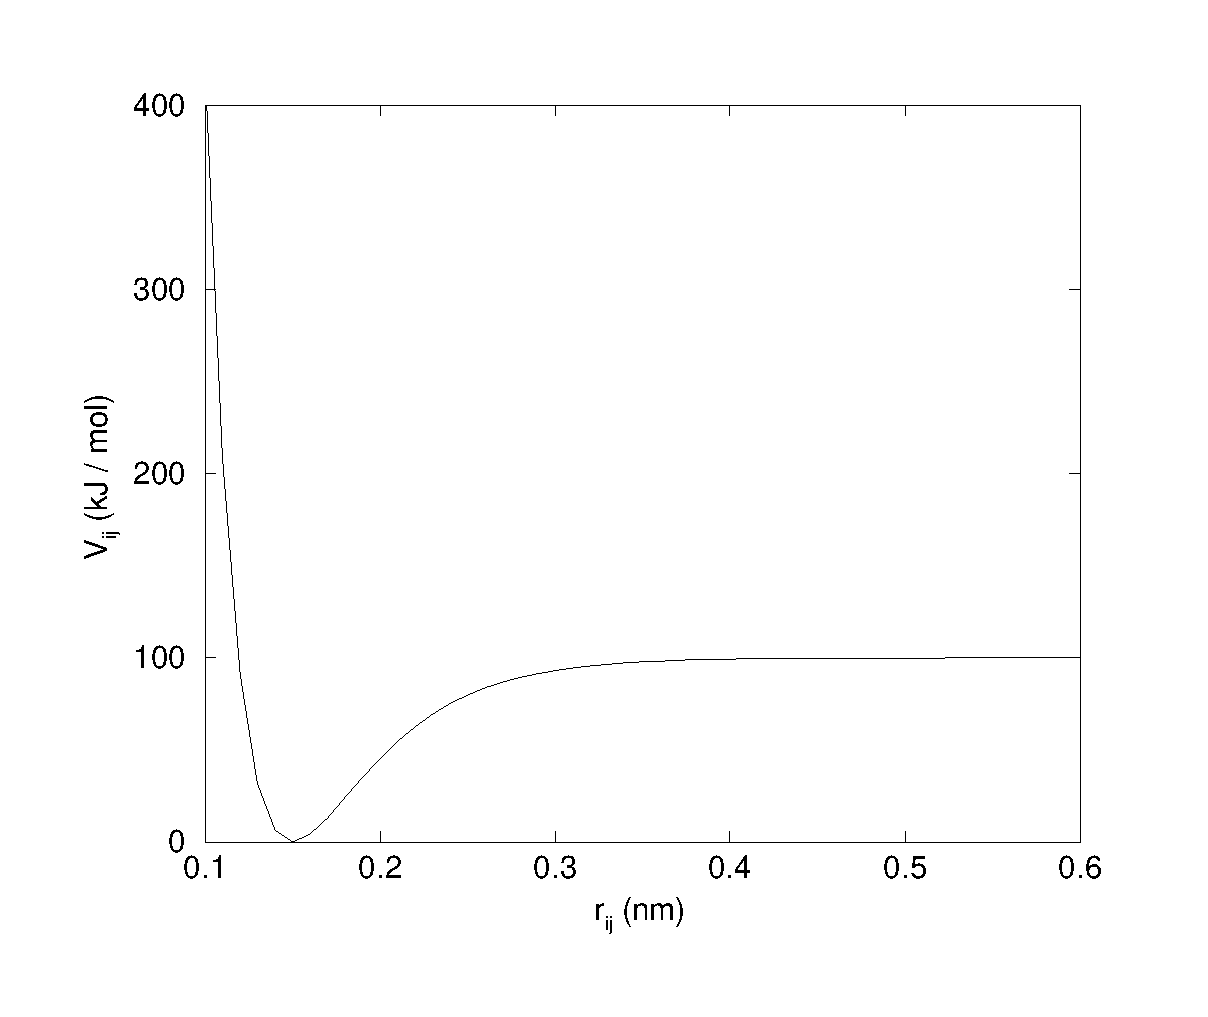
\includegraphics[width=7cm]{plots/f-morse}}
\caption{The Morse potential well, with bond length 0.15 nm.}
\label{fig:morse}
\end{figure}

\subsection{Cubic bond stretching potential}
\label{subsec:cubicbond}
Another anharmonic bond stretching potential that is slightly simpler
than the Morse potential adds a cubic term in the distance to the
simple harmonic form:
\beq
V_b~(\rij) = k^b_{ij}(\rij-b_{ij})^2 + k^b_{ij}k^{cub}_{ij}(\rij-b_{ij})^3
\eeq
A flexible \normindex{water} model (based on
the SPC water model~\cite{Berendsen81}) including 
a cubic bond stretching potential for the O-H bond
was developed by Ferguson~\cite{Ferguson95}. This model was found
to yield a reasonable infrared spectrum. The Ferguson water model is
available in the {\gromacs} library ({\tt flexwat-ferguson.itp}). 
It should be noted that the potential is asymmetric: overstretching leads to
infinitely low energies. The \swapindex{integration}{timestep} is therefore
limited to 1 fs.

The force corresponding to this potential is:
\beq
\ve{F}_i(\rvij) = 2k^b_{ij}(\rij-b_{ij})~\rnorm + 3k^b_{ij}k^{cub}_{ij}(\rij-b_{ij})^2~\rnorm
\eeq

\subsection{FENE bond stretching potential\index{FENE potential}}
\label{subsec:FENEbond}
In coarse-grained polymer simulations the beads are often connected
by a FENE (finitely extensible nonlinear elastic) potential~\cite{Warner72}:
\beq
V_{\mbox{\small FENE}}(\rij) =
  -\half k^b_{ij} b^2_{ij} \log\left(1 - \frac{\rij^2}{b^2_{ij}}\right)
\eeq
The potential looks complicated, but the expression for the force is simpler:
\beq
F_{\mbox{\small FENE}}(\rvij) =
  -k^b_{ij} \left(1 - \frac{\rij^2}{b^2_{ij}}\right)^{-1} \rvij
\eeq
At short distances the potential asymptotically goes to a harmonic
potential with force constant $k^b$, while it diverges at distance $b$.
%} % Brace matches ifthenelse test for gmxlite

\subsection{Harmonic angle potential}
\label{subsec:harmonicangle}
\newcommand{\tijk}{\theta_{ijk}}
The bond-\swapindex{angle}{vibration} between a triplet of atoms $i$ - $j$ - $k$
is also represented by a harmonic potential on the angle $\tijk$

\begin{figure}
\centerline{\raisebox{1cm}{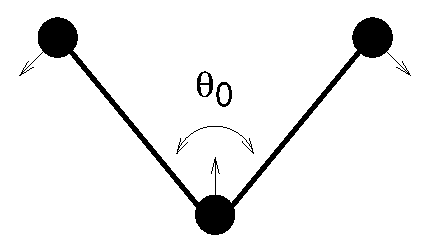
\includegraphics[width=5cm]{plots/angle}}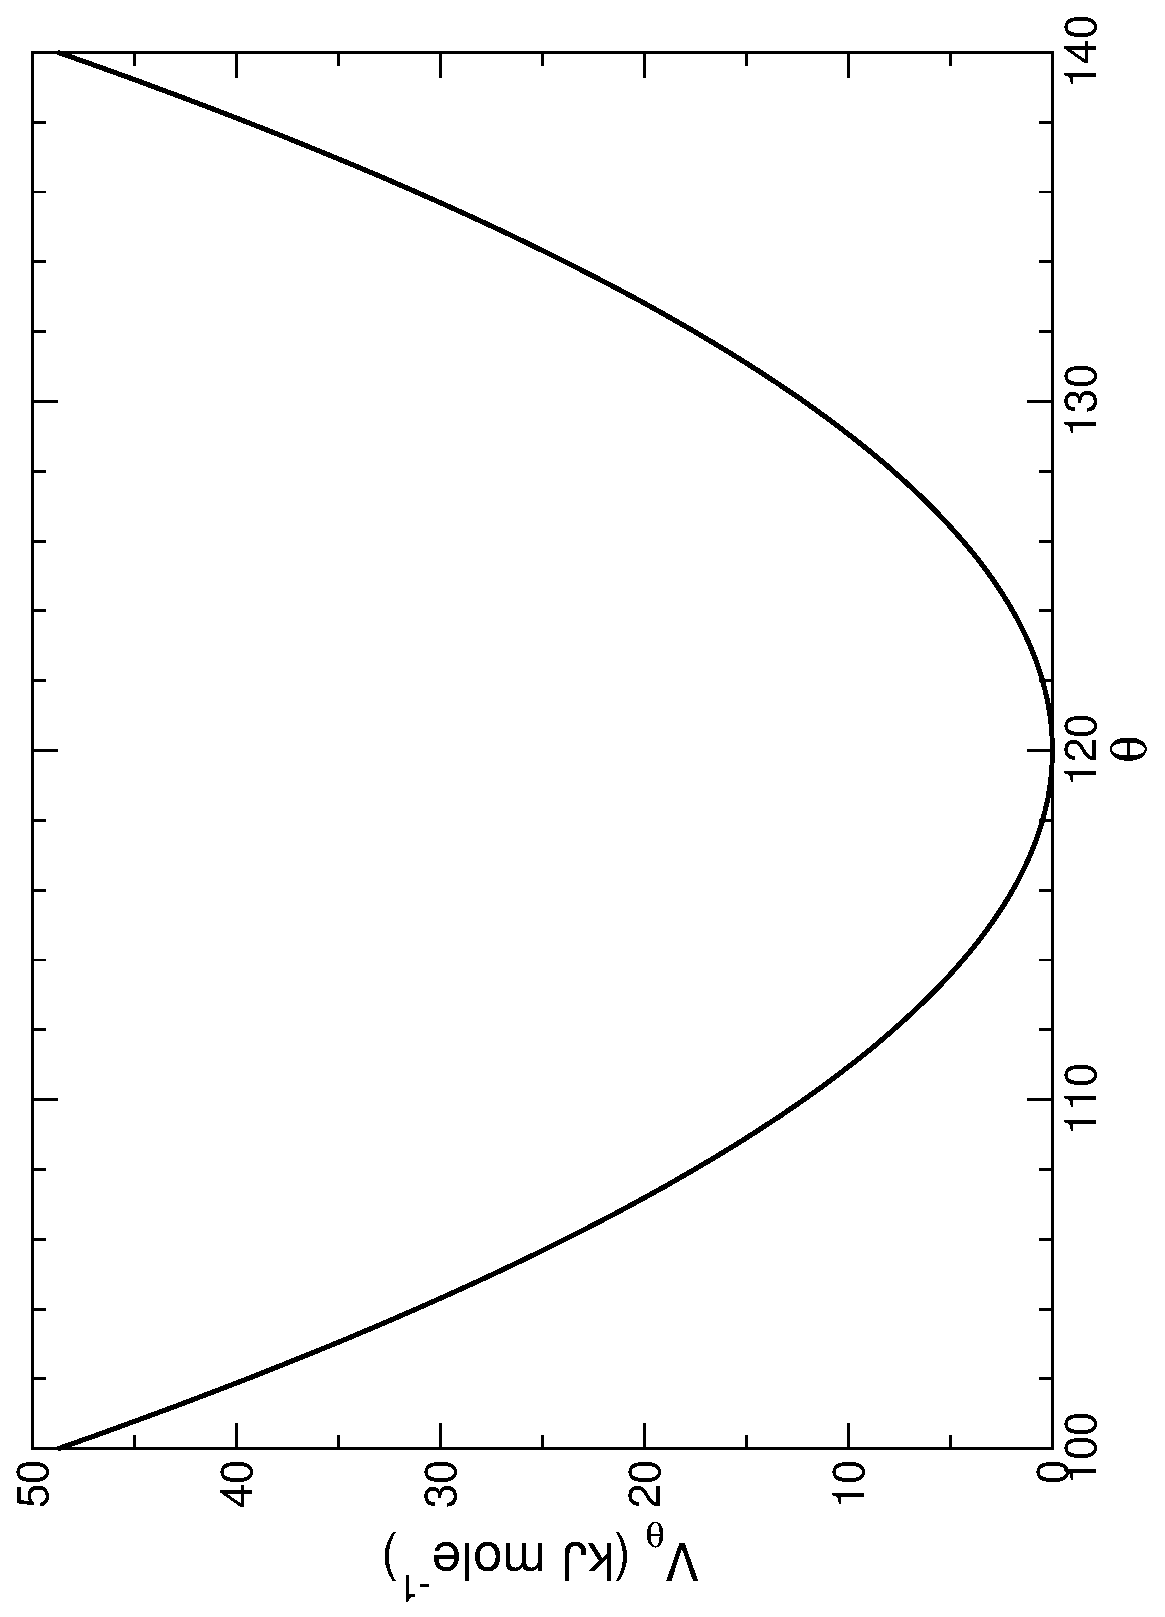
\includegraphics[width=7cm]{plots/f-angle}}
\caption[Angle vibration.]{Principle of angle vibration (left) and the
bond angle potential (right).}
\label{fig:angle}
\end{figure}

\beq
V_a(\tijk) = \half k^{\theta}_{ijk}(\tijk-\tijk^0)^2
\eeq
As the bond-angle vibration is represented by a harmonic potential, the
form is the same as the bond stretching (\figref{bstretch1}).

The force equations are given by the chain rule:
\beq
\begin{array}{l}
\Fvi    ~=~ -\displaystyle\frac{d V_a(\tijk)}{d \rvi}   \\
\Fvk    ~=~ -\displaystyle\frac{d V_a(\tijk)}{d \rvk}   \\
\Fvj    ~=~ -\Fvi-\Fvk
\end{array}
~ \mbox{ ~ where ~ } ~
 \tijk = \arccos \frac{(\rvij \cdot \ve{r}_{kj})}{r_{ij}r_{kj}}
\eeq
The numbering $i,j,k$ is in sequence of covalently bonded atoms. Atom
$j$ is in the middle; atoms $i$  and $k$ are at the ends (see \figref{angle}).
{\bf Note} that in the input in topology files, angles are given in degrees and
force constants in kJ/mol/rad$^2$.

%\ifthenelse{\equal{\gmxlite}{1}}{}{
\subsection{Cosine based angle potential}
\label{subsec:G96angle}
In the \gromosv{96} force field a simplified function is used to represent angle
vibrations:
\beq
V_a(\tijk) = \half k^{\theta}_{ijk}\left(\cos(\tijk) - \cos(\tijk^0)\right)^2
\label{eq:G96angle}
\eeq
where 
\beq
\cos(\tijk) = \frac{\rvij\cdot\ve{r}_{kj}}{\rij r_{kj}}
\eeq
The corresponding force can be derived by partial differentiation with respect
to the atomic positions. The force constants in this function are related
to the force constants in the harmonic form $k^{\theta,\mathrm{harm}}$
(\ssecref{harmonicangle}) by:
\beq
k^{\theta} \sin^2(\tijk^0) = k^{\theta,\mathrm{harm}}
\eeq
In the \gromosv{96} manual there is a much more complicated conversion formula
which is temperature dependent. The formulas are equivalent at 0 K
and the differences at 300 K are on the order of 0.1 to 0.2\%.
{\bf Note} that in the input in topology files, angles are given in degrees and
force constants in kJ/mol.

\subsection{Restricted bending potential}
\label{subsec:ReB}
The restricted bending (ReB) potential~\cite{MonicaGoga2013} prevents the bending angle $\theta$
from reaching the $180^{\circ}$ value. In this way, the numerical instabilities
due to the calculation of the torsion angle and potential are eliminated when
performing coarse-grained molecular dynamics simulations.

To systematically hinder the bending angles from reaching the $180^{\circ}$ value,
the bending potential \ref{eq:G96angle} is divided by a $\sin^2\theta$ factor:
%
\beq
V_{\rm ReB}(\theta_i) = \frac{1}{2} k_{\theta} \frac{(\cos\theta_i - \cos\theta_0)^2}{\sin^2\theta_i}.
\label{eq:ReB}
\eeq
%
Figure ~\figref{ReB} shows the comparison between the ReB potential, \ref{eq:ReB},
and the standard one \ref{eq:G96angle}.
%
\begin{figure}
\centerline{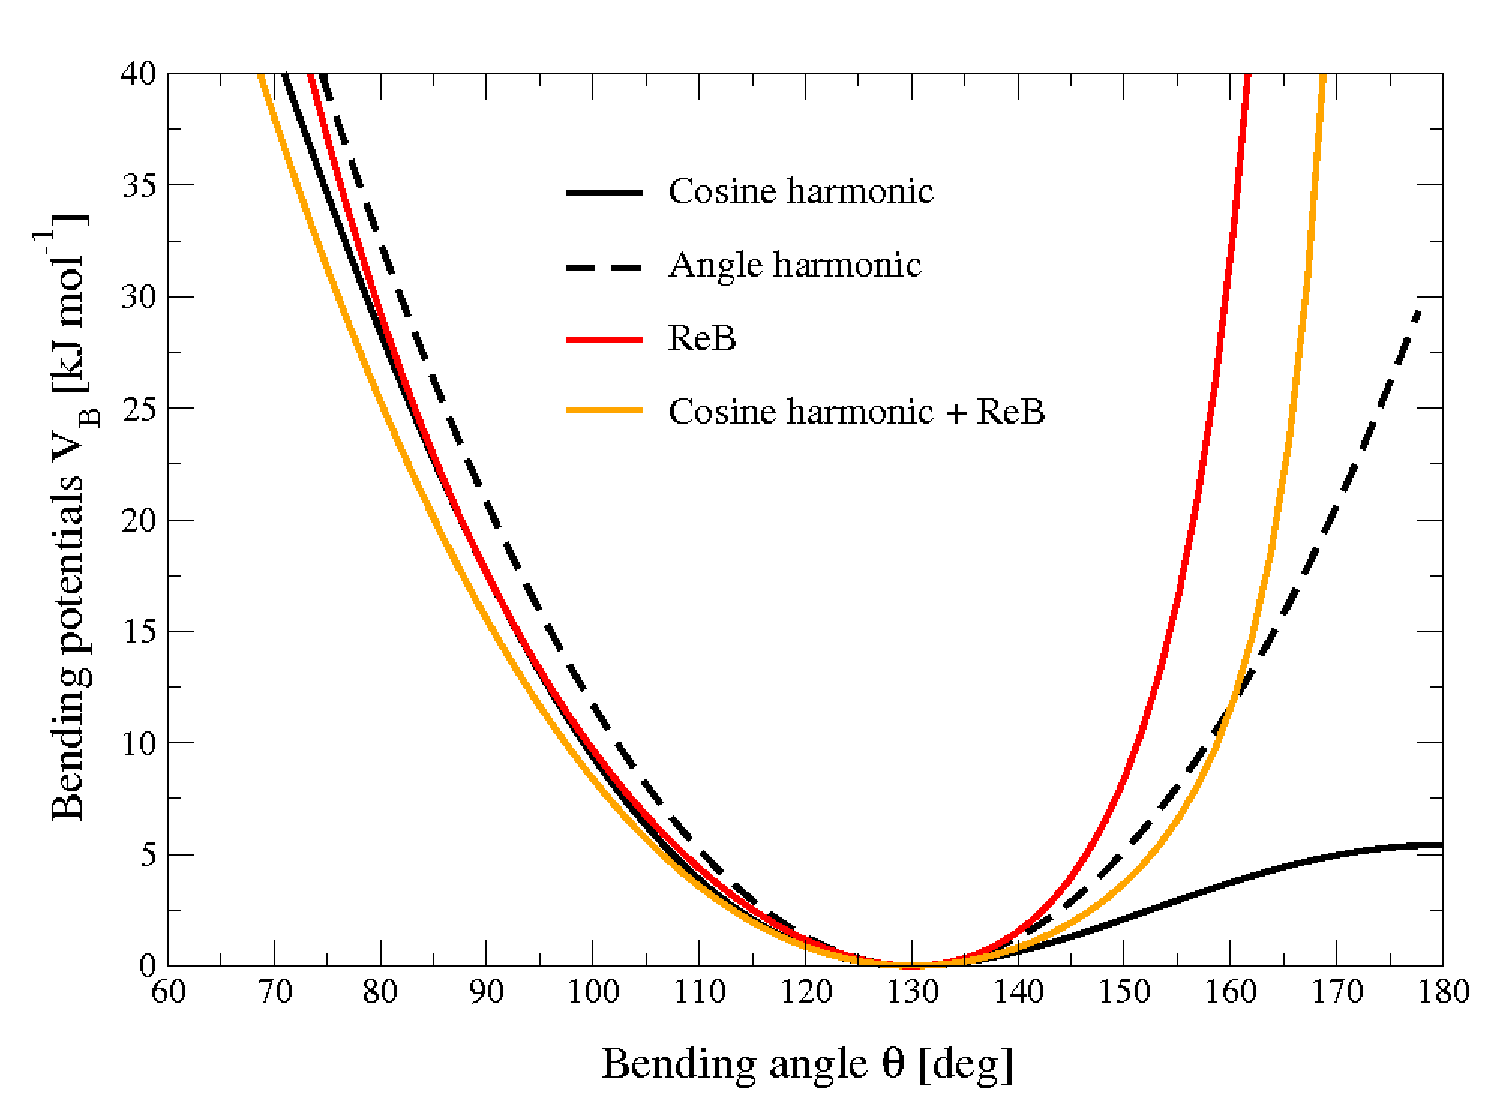
\includegraphics[width=10cm]{plots/fig-02}}
\vspace*{8pt}
\caption{Bending angle potentials: cosine harmonic (solid black line), angle harmonic
(dashed black line) and restricted bending (red) with the same bending constant
$k_{\theta}=85$ kJ mol$^{-1}$ and equilibrium angle $\theta_0=130^{\circ}$.
The orange line represents the sum of a cosine harmonic ($k =50$ kJ mol$^{-1}$)
with a restricted bending ($k =25$ kJ mol$^{-1}$) potential, both with $\theta_0=130^{\circ}$.}
\label{fig:ReB}
\end{figure}
%
The wall of the ReB potential is very repulsive in the region close to $180^{\circ}$ and,
as a result, the bending angles are kept within a safe interval, far from instabilities.
The power $2$ of $\sin\theta_i$ in the denominator has been chosen to guarantee this behavior
and allows an elegant differentiation:
%
\beq
F_{\rm ReB}(\theta_i) = \frac{2k_{\theta}}{\sin^4\theta_i}(\cos\theta_i - \cos\theta_0) (1 - \cos\theta_i\cos\theta_0) \frac{\partial \cos\theta_i}{\partial \vec r_{k}}.
\label{eq:diff_ReB}
\eeq
%
Due to its construction, the restricted bending potential cannot be used for equilibrium
$\theta_0$ values too close to $0^{\circ}$ or $180^{\circ}$ (from experience, at least $10^{\circ}$
difference is recommended). It is very important that, in the starting configuration,
all the bending angles have to be in the safe interval to avoid initial instabilities.
This bending potential can be used in combination with any form of torsion potential.
It will always prevent three consecutive particles from becoming collinear and,
as a result, any torsion potential will remain free of singularities.
It can be also added to a standard bending potential to affect the angle around $180^{\circ}$,
but to keep its original form around the minimum (see the orange curve in \figref{ReB}).


\subsection{Urey-Bradley potential}
\label{subsec:Urey-Bradley}
The \swapindex{Urey-Bradley bond-angle}{vibration} between a triplet
of atoms $i$ - $j$ - $k$ is represented by a harmonic potential on the
angle $\tijk$ and a harmonic correction term on the distance between
the atoms $i$ and $k$. Although this can be easily written as a simple
sum of two terms, it is convenient to have it as a single entry in the
topology file and in the output as a separate energy term. It is used mainly
in the CHARMm force field~\cite{BBrooks83}. The energy is given by:

\beq
V_a(\tijk) = \half k^{\theta}_{ijk}(\tijk-\tijk^0)^2 + \half k^{UB}_{ijk}(r_{ik}-r_{ik}^0)^2
\eeq

The force equations can be deduced from sections~\ssecref{harmonicbond}
and~\ssecref{harmonicangle}.

\subsection{Bond-Bond cross term}
\label{subsec:bondbondcross}
The bond-bond cross term for three particles $i, j, k$ forming bonds
$i-j$ and $k-j$ is given by~\cite{Lawrence2003b}:
\begin{equation}
V_{rr'} ~=~ k_{rr'} \left(\left|\ve{r}_{i}-\ve{r}_j\right|-r_{1e}\right) \left(\left|\ve{r}_{k}-\ve{r}_j\right|-r_{2e}\right)
\label{crossbb}
\end{equation}
where $k_{rr'}$ is the force constant, and $r_{1e}$ and $r_{2e}$ are the
equilibrium bond lengths of the $i-j$ and $k-j$ bonds respectively. The force
associated with this potential on particle $i$ is:
\begin{equation}
\ve{F}_{i} = -k_{rr'}\left(\left|\ve{r}_{k}-\ve{r}_j\right|-r_{2e}\right)\frac{\ve{r}_i-\ve{r}_j}{\left|\ve{r}_{i}-\ve{r}_j\right|}
\end{equation}
The force on atom $k$ can be obtained by swapping $i$ and $k$ in the above
equation. Finally, the force on atom $j$ follows from the fact that the sum
of internal forces should be zero: $\ve{F}_j = -\ve{F}_i-\ve{F}_k$.

\subsection{Bond-Angle cross term}
\label{subsec:bondanglecross}
The bond-angle cross term for three particles $i, j, k$ forming bonds
$i-j$ and $k-j$ is given by~\cite{Lawrence2003b}:
\begin{equation}
V_{r\theta} ~=~ k_{r\theta} \left(\left|\ve{r}_{i}-\ve{r}_k\right|-r_{3e} \right) \left(\left|\ve{r}_{i}-\ve{r}_j\right|-r_{1e} + \left|\ve{r}_{k}-\ve{r}_j\right|-r_{2e}\right)
\end{equation}
where $k_{r\theta}$ is the force constant, $r_{3e}$ is the $i-k$ distance,
and the other constants are the same as in Equation~\ref{crossbb}. The force
associated with the potential on atom $i$ is:
\begin{equation}
\ve{F}_{i} ~=~ -k_{r\theta}\left[\left(\left|\ve{r}_{i}-\ve{r}_{k}\right|-r_{3e}\right)\frac{\ve{r}_i-\ve{r}_j}{\left|\ve{r}_{i}-\ve{r}_j\right|} \\
+ \left(\left|\ve{r}_{i}-\ve{r}_j\right|-r_{1e} + \left|\ve{r}_{k}-\ve{r}_j\right|-r_{2e}\right)\frac{\ve{r}_i-\ve{r}_k}{\left|\ve{r}_{i}-\ve{r}_k\right|}\right]
\end{equation}

\subsection{Quartic angle potential}
\label{subsec:quarticangle}
For special purposes there is an angle potential
that uses a fourth order polynomial:
\beq
V_q(\tijk) ~=~ \sum_{n=0}^5 C_n (\tijk-\tijk^0)^n
\eeq
%} % Brace matches ifthenelse test for gmxlite

%% new commands %%%%%%%%%%%%%%%%%%%%%%
\newcommand{\rvkj}{{\bf r}_{kj}}
\newcommand{\rkj}{r_{kj}}
%%%%%%%%%%%%%%%%%%%%%%%%%%%%%%%%%%%%%%

\subsection{Improper dihedrals\swapindexquiet{improper}{dihedral}}
\label{sec:imp}
Improper dihedrals are meant to keep \swapindex{planar}{group}s ({\eg} 
aromatic rings) planar, or to prevent molecules from flipping over to their
\normindex{mirror image}s, see \figref{imp}.

\begin {figure}
\centerline{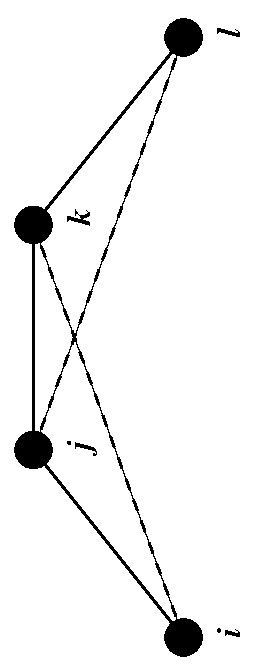
\includegraphics[width=4cm]{plots/ring-imp}\hspace{1cm}
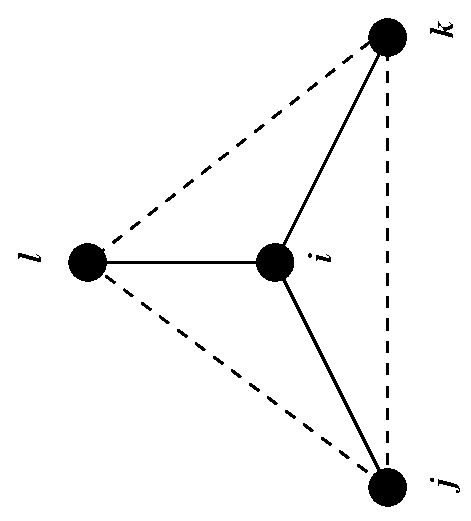
\includegraphics[width=3cm]{plots/subst-im}\hspace{1cm}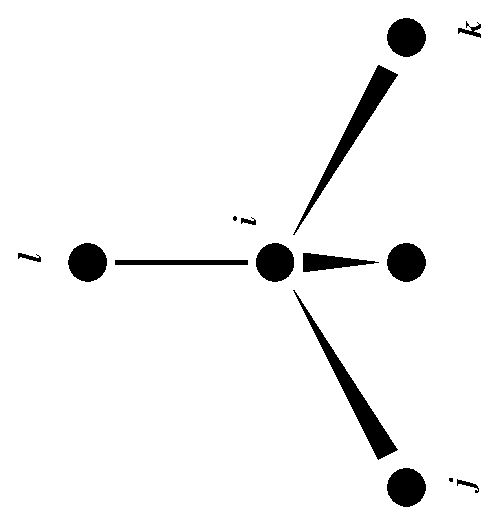
\includegraphics[width=3cm]{plots/tetra-im}}
\caption[Improper dihedral angles.]{Principle of improper
dihedral angles. Out of plane bending for rings (left), substituents
of rings (middle), out of tetrahedral (right). The improper dihedral
angle $\xi$ is defined as the angle between planes (i,j,k) and (j,k,l)
in all cases.}
\label{fig:imp}
\end {figure}

\subsubsection{Improper dihedrals: harmonic type}
\label{subsec:harmonicimproperdihedral}
The simplest improper dihedral potential is a harmonic potential; it is plotted in
\figref{imps}.
\beq
V_{id}(\xi_{ijkl}) = \half k_{\xi}(\xi_{ijkl}-\xi_0)^2
\eeq
Since the potential is harmonic it is discontinuous,
but since the discontinuity is chosen at 180$^\circ$ distance from $\xi_0$
this will never cause problems.
{\bf Note} that in the input in topology files, angles are given in degrees and
force constants in kJ/mol/rad$^2$.

\begin{figure}
\centerline{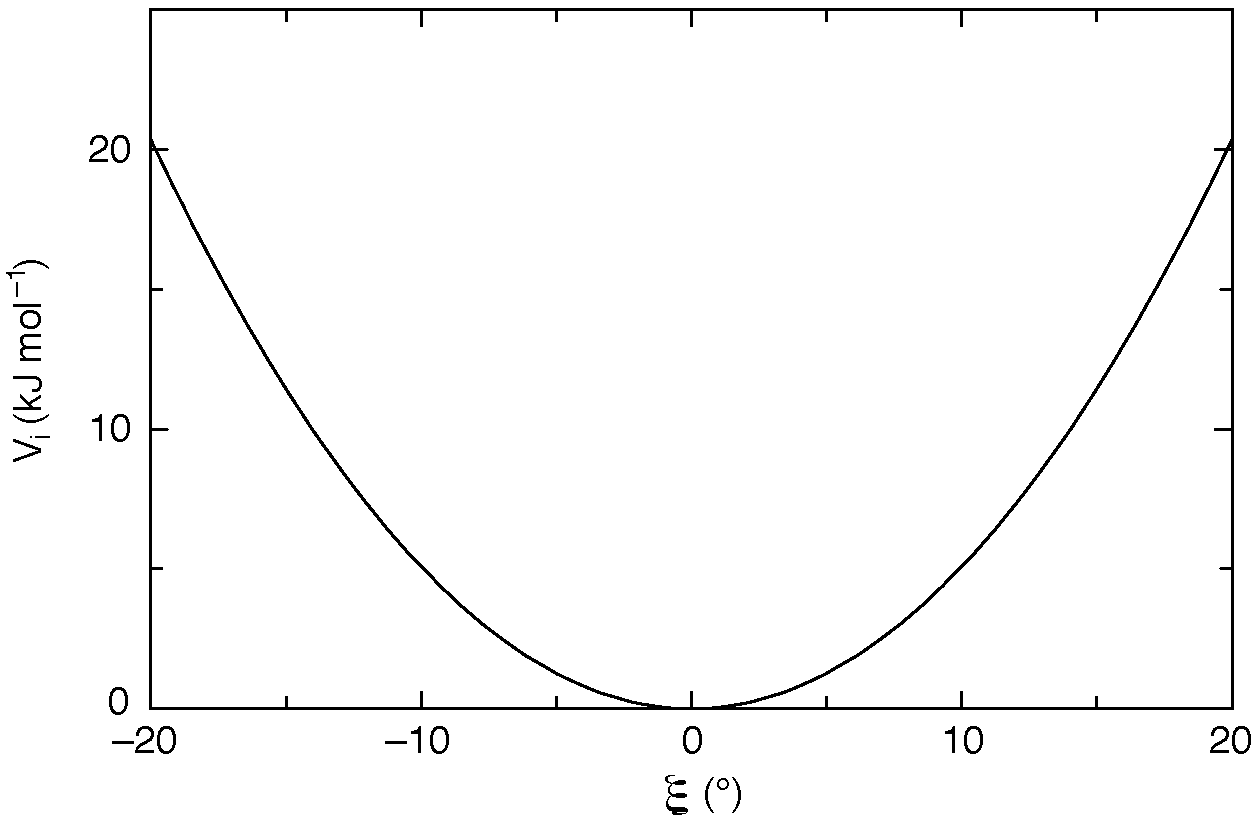
\includegraphics[width=8cm]{plots/f-imps}}
\caption{Improper dihedral potential.}
\label{fig:imps}
\end{figure}

\subsubsection{Improper dihedrals: periodic type}
\label{subsec:periodicimproperdihedral}
This potential is identical to the periodic proper dihedral (see below).
There is a separate dihedral type for this (type 4) only to be able
to distinguish improper from proper dihedrals in the parameter section
and the output.

\subsection{Proper dihedrals\swapindexquiet{proper}{dihedral}}
For the normal \normindex{dihedral} interaction there is a choice of
either the {\gromos} periodic function or a function based on
expansion in powers of $\cos \phi$ (the so-called Ryckaert-Bellemans
potential). This choice has consequences for the inclusion of special
interactions between the first and the fourth atom of the dihedral
quadruple. With the periodic {\gromos} potential a special 1-4
LJ-interaction must be included; with the Ryckaert-Bellemans potential
{\em for alkanes} the \normindex{1-4 interaction}s must be excluded
from the non-bonded list.  {\bf Note:} Ryckaert-Bellemans potentials
are also used in {\eg} the OPLS force field in combination with 1-4
interactions. You should therefore not modify topologies generated by
{\tt \normindex{pdb2gmx}} in this case.

\subsubsection{Proper dihedrals: periodic type}
\label{subsec:properdihedral}
Proper dihedral angles are defined according to the IUPAC/IUB
convention, where $\phi$ is the angle between the $ijk$ and the $jkl$
planes, with {\bf zero} corresponding to the {\em cis} configuration
($i$ and $l$ on the same side). There are two dihedral function types
in {\gromacs} topology files. There is the standard type 1 which behaves
like any other bonded interactions. For certain force fields, type 9
is useful. Type 9 allows multiple potential functions to be applied
automatically to a single dihedral in the {\tt [ dihedral ]} section
when multiple parameters are defined for the same atomtypes
in the {\tt [ dihedraltypes ]} section.

\begin{figure}
\centerline{\raisebox{1cm}{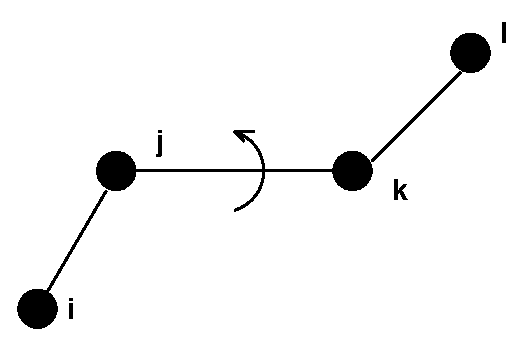
\includegraphics[width=5cm]{plots/dih}}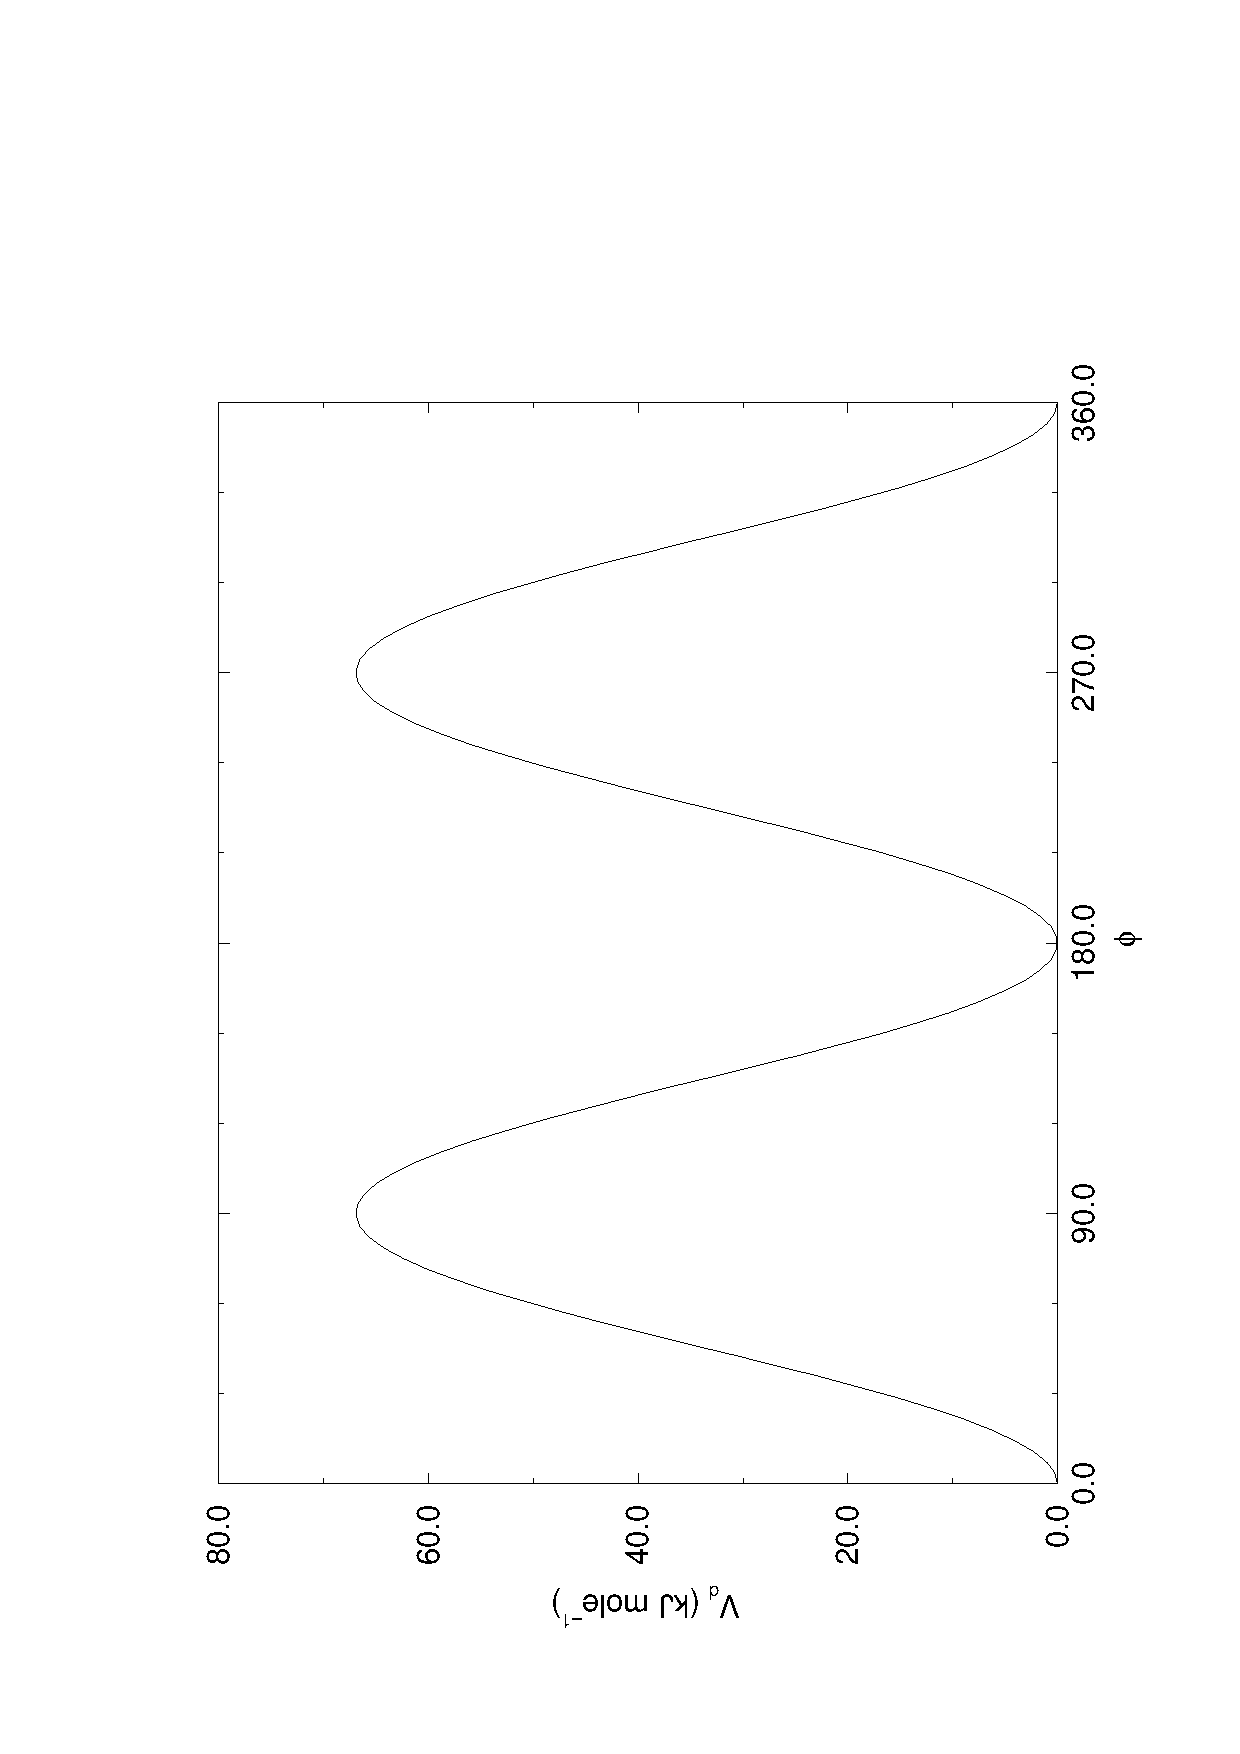
\includegraphics[width=7cm]{plots/f-dih}}
\caption[Proper dihedral angle.]{Principle of proper dihedral angle
(left, in {\em trans} form) and the dihedral angle potential (right).} 
\label{fig:pdihf}
\end{figure}
\beq
V_d(\phi_{ijkl}) = k_{\phi}(1 + \cos(n \phi - \phi_s))
\eeq

%\ifthenelse{\equal{\gmxlite}{1}}{}{
\subsubsection{Proper dihedrals: Ryckaert-Bellemans function}
\label{subsec:RBdihedral}
For alkanes, the following proper dihedral potential is often used
(see \figref{rbdih}):
\beq
V_{rb}(\phi_{ijkl}) = \sum_{n=0}^5 C_n( \cos(\psi ))^n,
\eeq 
where $\psi = \phi - 180^\circ$.  \\
{\bf Note:} A conversion from one convention to another can be achieved by 
multiplying every coefficient \( \displaystyle C_n \) 
by \( \displaystyle (-1)^n \).

An example of constants for $C$ is given in \tabref{crb}.

\begin{table}
\centerline{
\begin{tabular}{|lr|lr|lr|}
\dline
$C_0$   & 9.28  & $C_2$   & -13.12  & $C_4$   & 26.24   \\
$C_1$   & 12.16 & $C_3$   & -3.06   & $C_5$   & -31.5   \\
\dline
\end{tabular}
}
\caption{Constants for Ryckaert-Bellemans potential (kJ mol$^{-1}$).}
\label{tab:crb}
\end{table}

\begin{figure}
\centerline{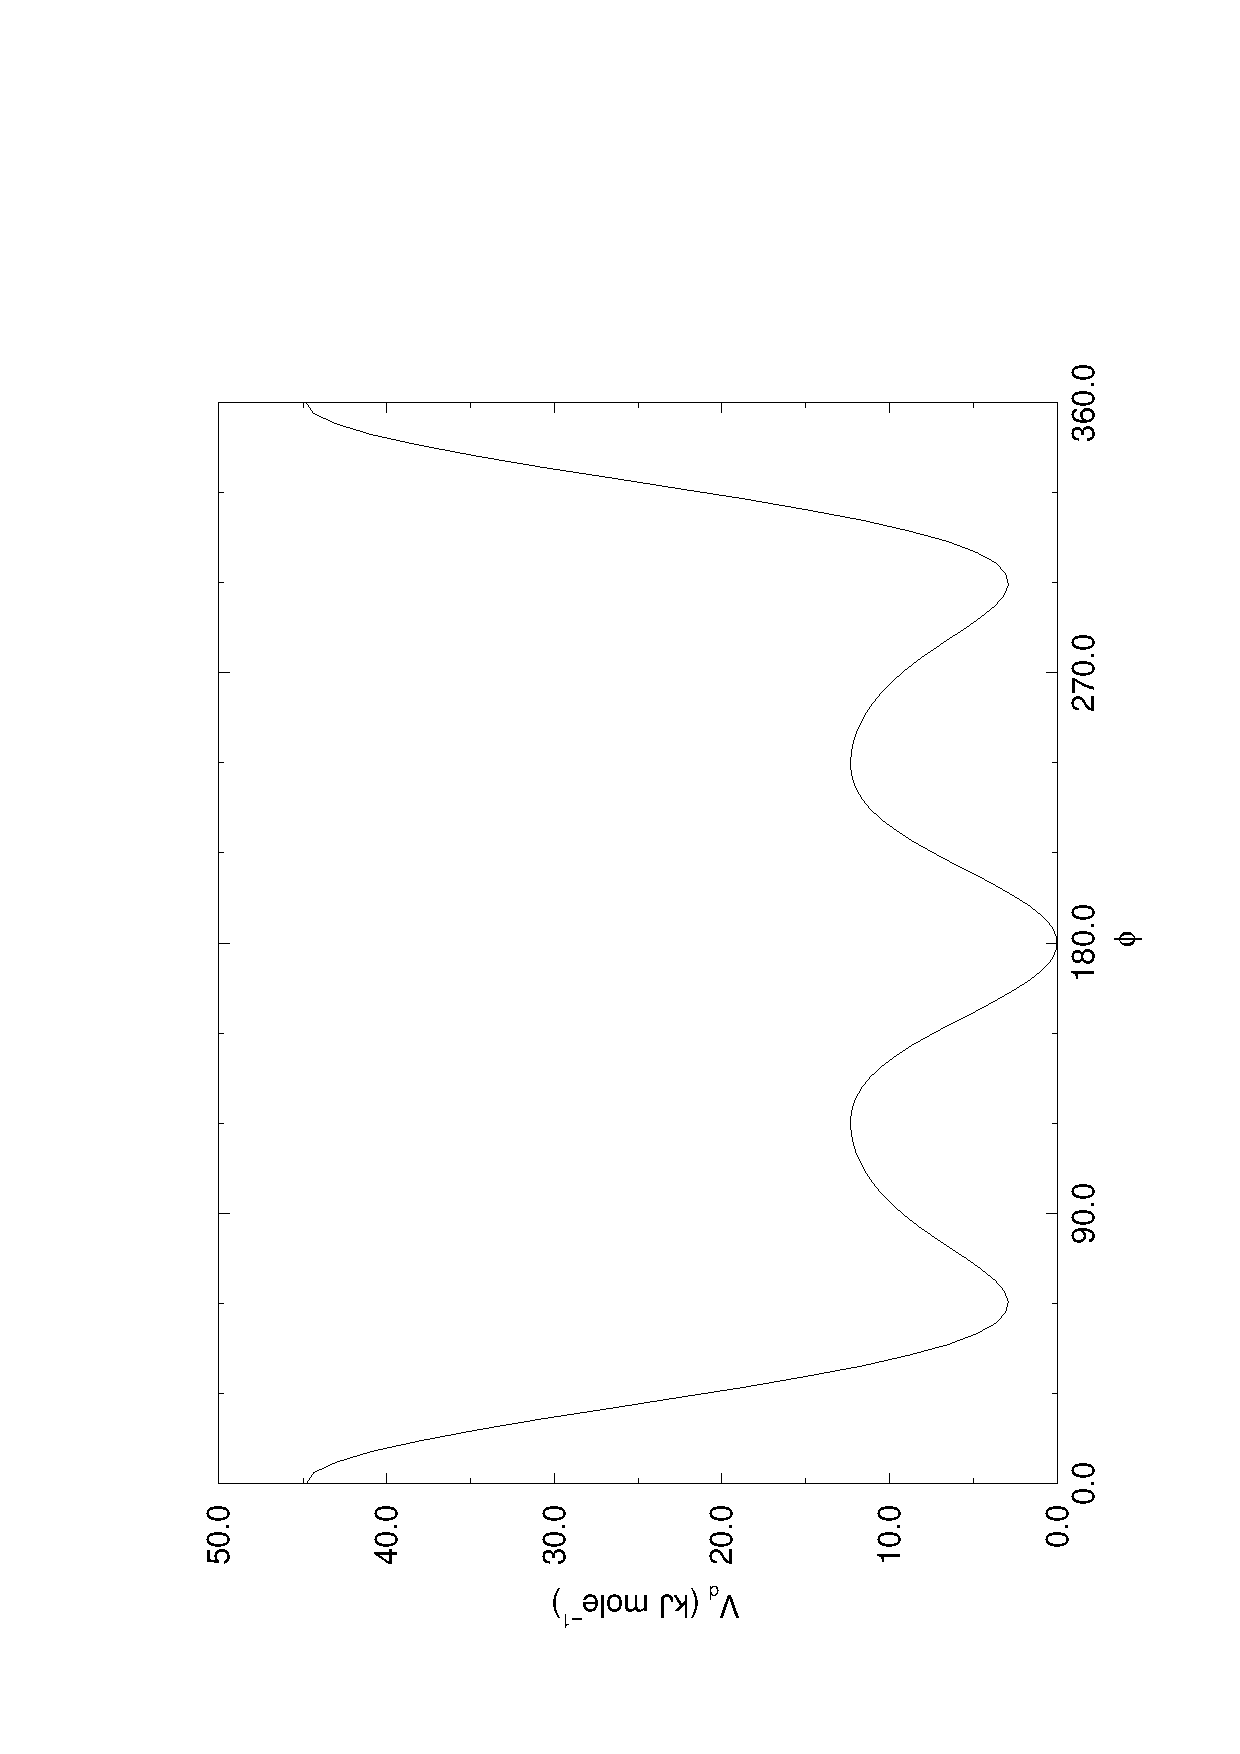
\includegraphics[width=8cm]{plots/f-rbs}}
\caption{Ryckaert-Bellemans dihedral potential.}
\label{fig:rbdih}
\end{figure}

({\bf Note:} The use of this potential implies exclusion of LJ interactions
between the first and the last atom of the dihedral, and $\psi$ is defined
according to the ``polymer convention'' ($\psi_{trans}=0$).)

The RB dihedral function can also be used to include Fourier dihedrals
(see below):
\beq
V_{rb} (\phi_{ijkl}) ~=~ \frac{1}{2} \left[F_1(1+\cos(\phi)) + F_2(
1-\cos(2\phi)) + F_3(1+\cos(3\phi)) + F_4(1-\cos(4\phi))\right]
\eeq
Because of the equalities \( \cos(2\phi) = 2\cos^2(\phi) - 1 \),
\( \cos(3\phi) = 4\cos^3(\phi) - 3\cos(\phi) \) and
\( \cos(4\phi) = 8\cos^4(\phi) - 8\cos^2(\phi) + 1 \)
one can translate the OPLS parameters to 
Ryckaert-Bellemans parameters as follows:
\beq
\displaystyle
\begin{array}{rcl}
\displaystyle C_0&=&F_2 + \frac{1}{2} (F_1 + F_3)\\
\displaystyle C_1&=&\frac{1}{2} (- F_1 + 3 \, F_3)\\
\displaystyle C_2&=& -F_2 + 4 \, F_4\\
\displaystyle C_3&=&-2 \, F_3\\
\displaystyle C_4&=&-4 \, F_4\\
\displaystyle C_5&=&0
\end{array}
\eeq 
with OPLS parameters in protein convention and RB parameters in
polymer convention (this yields a minus sign for the odd powers of 
cos$(\phi)$).\\
\noindent{\bf Note:} Mind the conversion from {\bf kcal mol$^{-1}$} for 
literature OPLS and RB parameters to {\bf kJ mol$^{-1}$} in {\gromacs}.\\
%} % Brace matches ifthenelse test for gmxlite

\subsubsection{Proper dihedrals: Fourier function}
\label{subsec:Fourierdihedral}
The OPLS potential function is given as the first three
or four~\cite{Jorgensen2005a} cosine terms of a Fourier series.
In {\gromacs} the four term function is implemented:
\beq
V_{F} (\phi_{ijkl}) ~=~ \frac{1}{2} \left[C_1(1+\cos(\phi)) + C_2(
1-\cos(2\phi)) + C_3(1+\cos(3\phi)) + C_4(1+\cos(4\phi))\right],
\eeq
%\ifthenelse{\equal{\gmxlite}{1}}{}{
Internally, {\gromacs}
uses the Ryckaert-Bellemans code
to compute Fourier dihedrals (see above), because this is more efficient.\\
\noindent{\bf Note:} Mind the conversion from {\emph kcal mol$^{-1}$} for 
literature OPLS parameters to {\bf kJ mol$^{-1}$} in {\gromacs}.\\

\subsubsection{Proper dihedrals: Restricted torsion potential}
\label{subsec:ReT}
In a manner very similar to the restricted bending potential (see \ref{subsec:ReB}),
a restricted torsion/dihedral potential is introduced:
%
\beq
V_{\rm ReT}(\phi_i) = \frac{1}{2} k_{\phi} \frac{(\cos\phi_i - \cos\phi_0)^2}{\sin^2\phi_i}
\label{eq:ReT}
\eeq
%
with the advantages of being a function of $\cos\phi$ (no problems taking the derivative of $\sin\phi$)
and of keeping the torsion angle at only one minimum value. In this case, the factor $\sin^2\phi$ does
not allow the dihedral angle to move from the [$-180^{\circ}$:0] to [0:$180^{\circ}$] interval, i.e. it cannot have maxima both at $-\phi_0$ and $+\phi_0$ maxima, but only one of them.
For this reason, all the dihedral angles of the starting configuration should have their values in the
desired angles interval and the the equilibrium $\phi_0$ value should not be too close to the interval limits
(as for the restricted bending potential, described in \ref{subsec:ReB}, at least $10^{\circ}$ difference is recommended).

\subsubsection{Proper dihedrals: Combined bending-torsion potential}
\label{subsec:CBT}
When the four particles forming the dihedral angle become collinear (this situation will never happen in
atomistic simulations, but it can occur in coarse-grained simulations) the calculation of the
torsion angle and potential leads to numerical instabilities.
One way to avoid this is to use the restricted bending potential (see \ref{subsec:ReB})
that prevents the dihedral
from reaching the $180^{\circ}$ value.

Another way is to disregard any effects of the dihedral becoming ill-defined,
keeping the dihedral force and potential calculation continuous in entire angle range
by coupling the torsion potential (in a cosine form) with the bending potentials of the
adjacent bending angles in a unique expression:
%
\beq
V_{\rm CBT}(\theta_{i-1}, \theta_i, \phi_i) = k_{\phi} \sin^3\theta_{i-1} \sin^3\theta_{i} \sum_{n=0}^4 { a_n \cos^n\phi_i}.
\label{eq:CBT}
\eeq
%
This combined bending-torsion (CBT) potential has been proposed by~\cite{BulacuGiessen2005}
for polymer melt simulations and is extensively described in~\cite{MonicaGoga2013}.

This potential has two main advantages:
\begin{itemize}
\item
it does not only depend on the dihedral angle $\phi_i$ (between the $i-2$, $i-1$, $i$ and $i+1$ beads)
but also on the bending angles $\theta_{i-1}$ and $\theta_i$ defined from three adjacent beads
($i-2$, $i-1$ and $i$, and $i-1$, $i$ and $i+1$, respectively).
The two $\sin^3\theta$ pre-factors, tentatively suggested by~\cite{ScottScheragator1966} and theoretically
discussed by~\cite{PaulingBond}, cancel the torsion potential and force when either of the two bending angles
approaches the value of $180^\circ$.
\item
its dependence on $\phi_i$ is expressed through a polynomial in $\cos\phi_i$ that avoids the singularities in
$\phi=0^\circ$ or $180^\circ$ in calculating the torsional force.
\end{itemize}

These two  properties make the CBT potential well-behaved for MD simulations with weak constraints
on the bending angles or even for steered / non-equilibrium MD in which the bending and torsion angles suffer major
modifications.
When using the CBT potential, the bending potentials for the adjacent $\theta_{i-1}$ and $\theta_i$ may have any form.
It is also possible to leave out the two angle bending terms ($\theta_{i-1}$ and $\theta_{i}$) completely.
\figref{CBT} illustrates the difference between a torsion potential with and without the $\sin^{3}\theta$ factors
(blue and gray curves, respectively).
%
\begin{figure}
\centerline{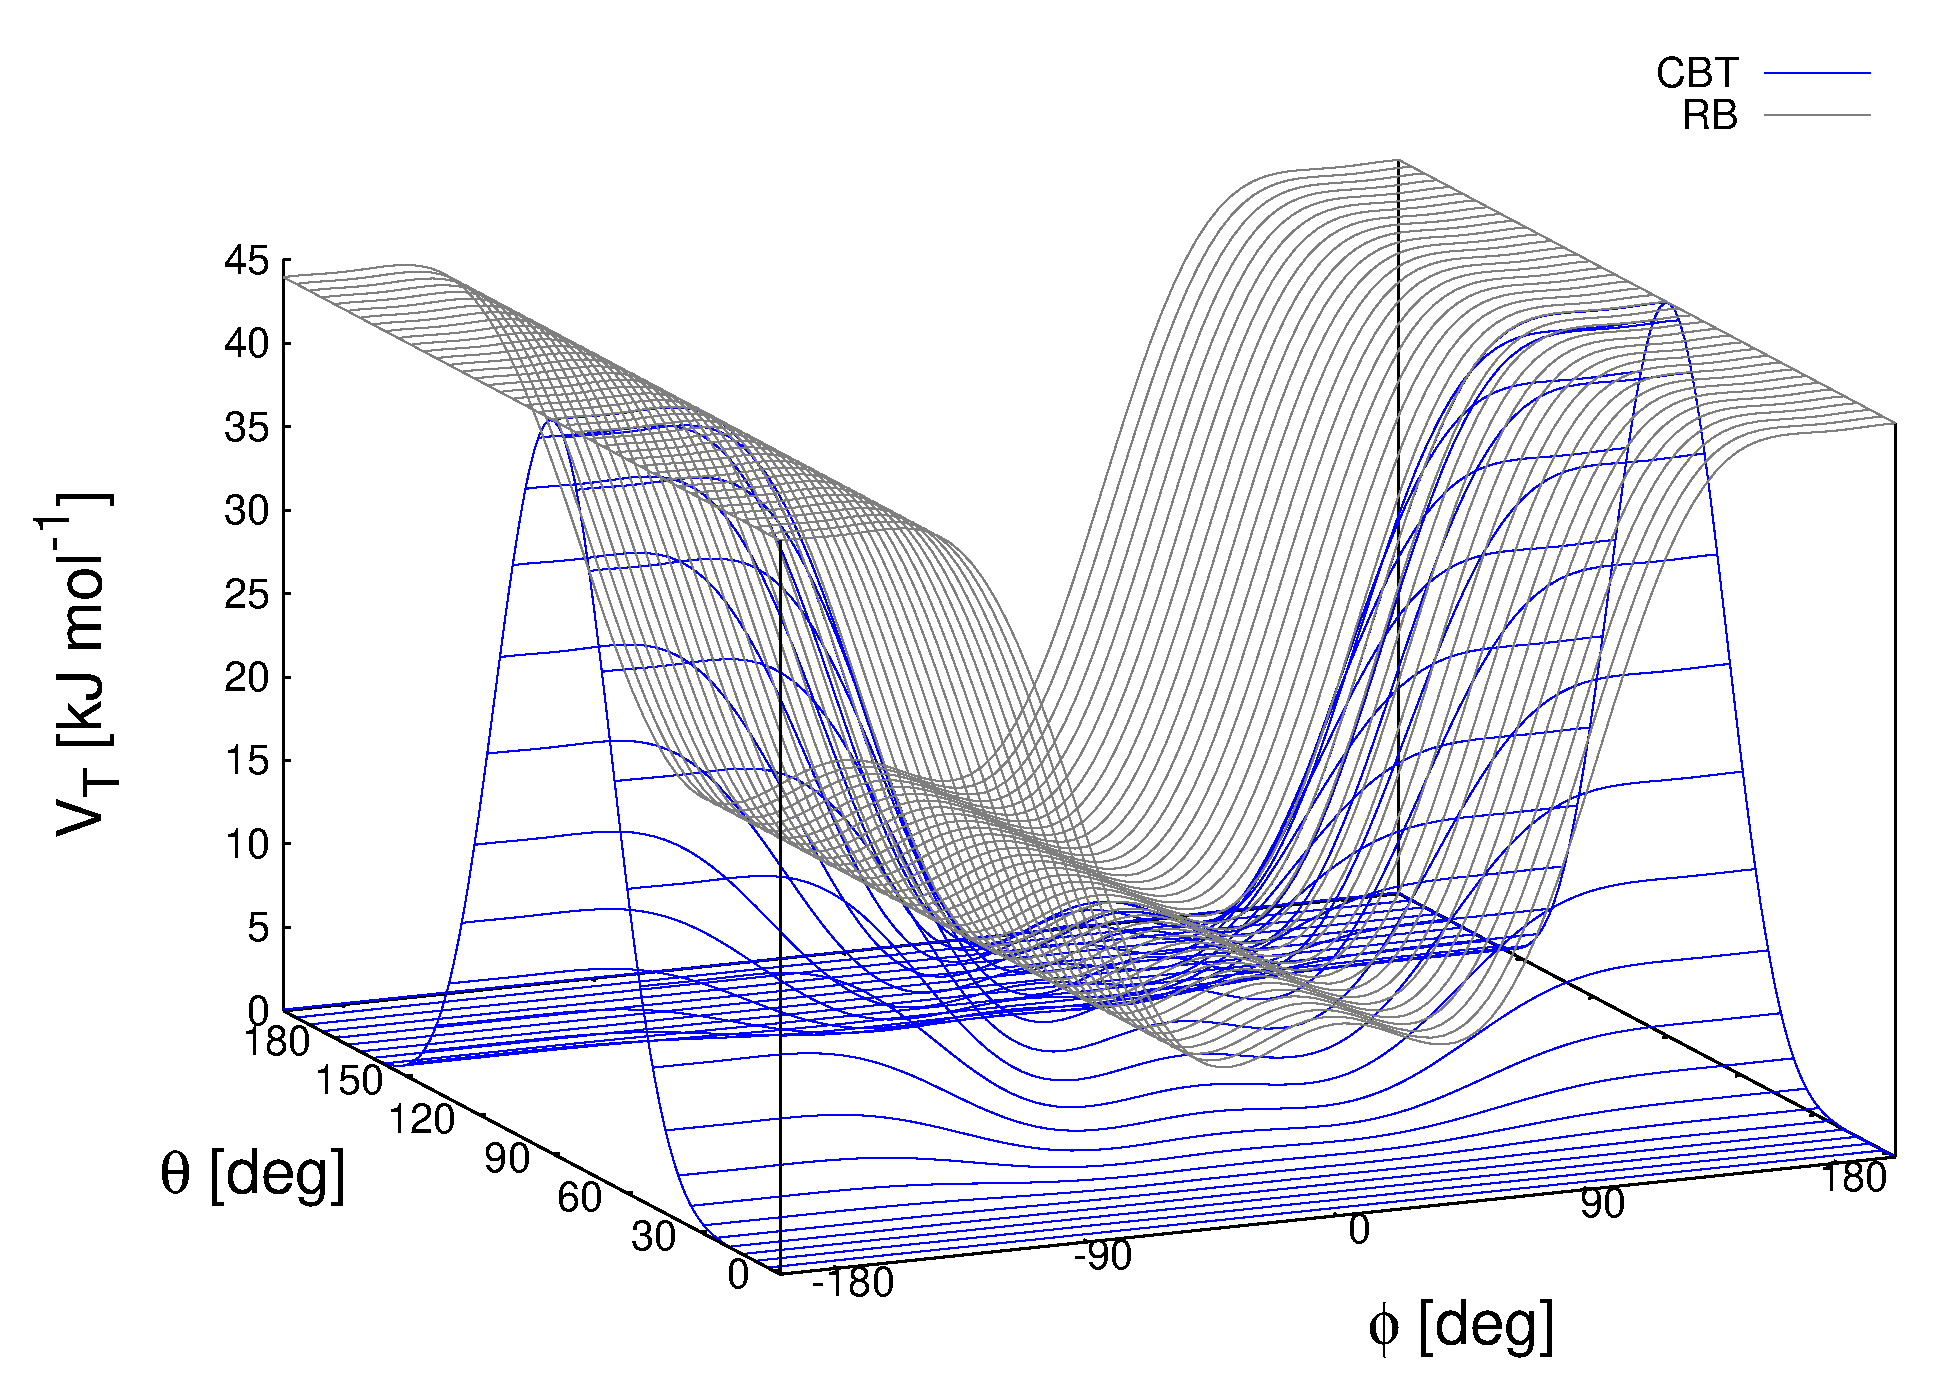
\includegraphics[width=10cm]{plots/fig-04}}
\caption{Blue: surface plot of the combined bending-torsion potential
(\ref{eq:CBT} with $k = 10$ kJ mol$^{-1}$, $a_0=2.41$, $a_1=-2.95$, $a_2=0.36$, $a_3=1.33$)
when, for simplicity, the bending angles behave the same ($\theta_1=\theta_2=\theta$).
Gray: the same torsion potential without the $\sin^{3}\theta$ terms (Ryckaert-Bellemans type).
$\phi$ is the dihedral angle.}
\label{fig:CBT}
\end{figure}
%
Additionally, the derivative of $V_{CBT}$ with respect to the Cartesian variables is straightforward:
%
\begin{equation}
\frac{\partial V_{\rm CBT}(\theta_{i-1},\theta_i,\phi_i)} {\partial \vec r_{l}} = \frac{\partial V_{\rm CBT}}{\partial \theta_{i-1}} \frac{\partial \theta_{i-1}}{\partial \vec r_{l}} +
                                                                                  \frac{\partial V_{\rm CBT}}{\partial \theta_{i  }} \frac{\partial \theta_{i  }}{\partial \vec r_{l}} +
                                                                                  \frac{\partial V_{\rm CBT}}{\partial \phi_{i    }} \frac{\partial \phi_{i    }}{\partial \vec r_{l}}
\label{eq:force_cbt}
\end{equation}
%
The CBT is based on a cosine form without multiplicity, so it can only be symmetrical around $0^{\circ}$.
To obtain an asymmetrical dihedral angle distribution (e.g. only one maximum in [$-180^{\circ}$:$180^{\circ}$] interval),
a standard torsion potential such as harmonic angle  or  periodic cosine potentials should be used instead of a CBT potential.
However, these two forms have the inconveniences of the force derivation ($1/\sin\phi$) and of the alignment of beads
($\theta_i$ or $\theta_{i-1} = 0^{\circ}, 180^{\circ}$).
Coupling such non-$\cos\phi$ potentials with $\sin^3\theta$ factors does not improve simulation stability since there are
cases in which $\theta$ and $\phi$ are simultaneously $180^{\circ}$. The integration at this step would be possible
(due to the cancelling of the torsion potential) but the next step would be singular
($\theta$ is not $180^{\circ}$ and $\phi$ is very close to $180^{\circ}$).

%\ifthenelse{\equal{\gmxlite}{1}}{}{
\subsection{Tabulated bonded interaction functions\index{tabulated bonded interaction function}}
\label{subsec:tabulatedinteraction}
For full flexibility, any functional shape can be used for
bonds, angles and dihedrals through user-supplied tabulated functions.
The functional shapes are:
\bea
V_b(r_{ij})      &=& k \, f^b_n(r_{ij}) \\
V_a(\tijk)       &=& k \, f^a_n(\tijk) \\
V_d(\phi_{ijkl}) &=& k \, f^d_n(\phi_{ijkl})
\eea
where $k$ is a force constant in units of energy
and $f$ is a cubic spline function; for details see \ssecref{cubicspline}.
For each interaction, the force constant $k$ and the table number $n$
are specified in the topology.
There are two different types of bonds, one that generates exclusions (type 8)
and one that does not (type 9).
For details see \tabref{topfile2}.
The table files are supplied to the {\tt mdrun} program.
After the table file name an underscore, the letter ``b'' for bonds,
``a'' for angles or ``d'' for dihedrals and the table number are appended.
For example, for a bond with $n=0$ (and using the default table file name)
the table is read from the file {\tt table_b0.xvg}.  Multiple tables can be
supplied simply by using different values of $n$, and are applied to the appropriate
bonds, as specified in the topology (\tabref{topfile2}).
The format for the table files is three columns with $x$, $f(x)$, $-f'(x)$,
where $x$ should be uniformly-spaced. Requirements for entries in the topology
are given in~\tabref{topfile2}. 
The setup of the tables is as follows:
\\{\bf bonds}:
$x$ is the distance in nm. For distances beyond the table length,
{\tt mdrun} will quit with an error message.
\\{\bf angles}:
$x$ is the angle in degrees. The table should go from
0 up to and including 180 degrees; the derivative is taken in degrees.
\\{\bf dihedrals}:
$x$ is the dihedral angle in degrees. The table should go from
-180 up to and including 180 degrees;
the IUPAC/IUB convention is used, {\ie} zero is cis,
the derivative is taken in degrees.
%} % Brace matches ifthenelse test for gmxlite

\section{Restraints}
Special potentials are used for imposing restraints on the motion of
the system, either to avoid disastrous deviations, or to include
knowledge from experimental data. In either case they are not really
part of the force field and the reliability of the parameters is not
important. The potential forms, as implemented in {\gromacs}, are
mentioned just for the sake of completeness. Restraints and constraints
refer to quite different algorithms in {\gromacs}.

\subsection{Position restraints\swapindexquiet{position}{restraint}}
\label{subsec:positionrestraint}
These are used to restrain particles to fixed reference positions
$\ve{R}_i$. They can be used during equilibration in order to avoid
drastic rearrangements of critical parts ({\eg} to restrain motion
in a protein that is subjected to large solvent forces when the
solvent is not yet equilibrated). Another application is the
restraining of particles in a shell around a region that is simulated
in detail, while the shell is only approximated because it lacks
proper interaction from missing particles outside the
shell. Restraining will then maintain the integrity of the inner
part. For spherical shells, it is a wise procedure to make the force
constant depend on the radius, increasing from zero at the inner
boundary to a large value at the outer boundary. This feature has
not, however, been implemented in {\gromacs}.
\newcommand{\unitv}[1]{\hat{\bf #1}}
\newcommand{\halfje}[1]{\frac{#1}{2}}

The following form is used: 
\beq
V_{pr}(\ve{r}_i) = \halfje{1}k_{pr}|\rvi-\ve{R}_i|^2
\eeq
The potential is plotted in \figref{positionrestraint}.

\begin{figure}
\centerline{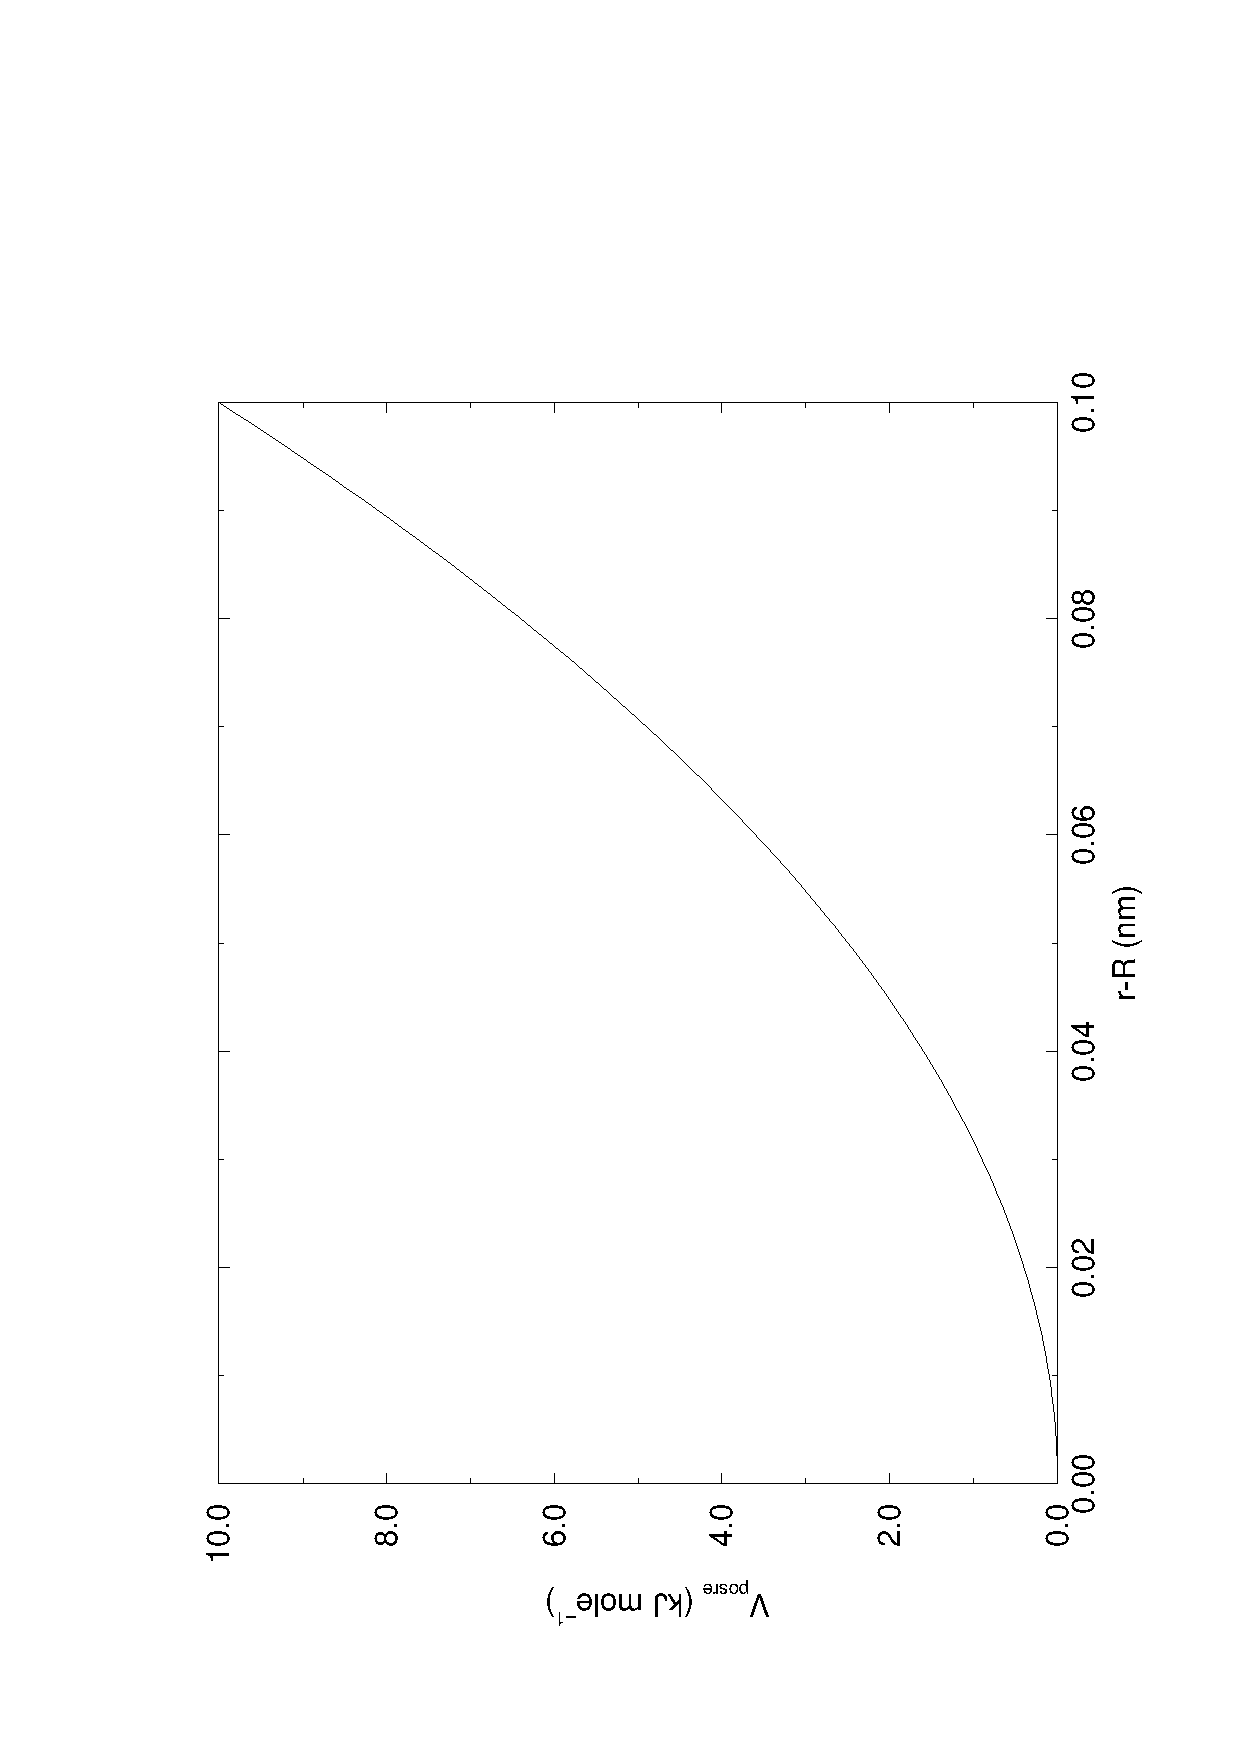
\includegraphics[width=8cm]{plots/f-pr}}
\caption{Position restraint potential.}
\label{fig:positionrestraint}
\end{figure}

The potential form can be rewritten without loss of generality as:
\beq
V_{pr}(\ve{r}_i) = \halfje{1} \left[ k_{pr}^x (x_i-X_i)^2 ~\unitv{x} + k_{pr}^y (y_i-Y_i)^2 ~\unitv{y} + k_{pr}^z (z_i-Z_i)^2 ~\unitv{z}\right]
\eeq

Now the forces are:
\beq
\begin{array}{rcl}
F_i^x &=& -k_{pr}^x~(x_i - X_i) \\
F_i^y &=& -k_{pr}^y~(y_i - Y_i) \\
F_i^z &=& -k_{pr}^z~(z_i - Z_i)
\end{array}
\eeq
Using three different force constants the position 
restraints can be turned on or off
in each spatial dimension; this means that atoms can be harmonically
restrained to a plane or a line.
Position restraints are applied to a special fixed list of atoms. Such a
list is usually generated by the {\tt \normindex{pdb2gmx}} program.

\subsection{\swapindex{Flat-bottomed}{position restraint}s}
\label{subsec:fbpositionrestraint}
Flat-bottomed position restraints can be used to restrain particles to 
part of the simulation volume. No force acts on the restrained
particle within the flat-bottomed region of the potential, however a
harmonic force acts to move the particle to the flat-bottomed region
if it is outside it. It is possible to apply normal and
flat-bottomed position restraints on the same particle (however, only
with the same reference position $\ve{R}_i$). The following general potential
is used (Figure~\ref{fig:fbposres}A):
\beq
 V_\mathrm{fb}(\ve{r}_i) = \frac{1}{2}k_\mathrm{fb} [d_g(\ve{r}_i;\ve{R}_i) - r_\mathrm{fb}]^2\,H[d_g(\ve{r}_i;\ve{R}_i) - r_\mathrm{fb}],
\eeq
where $\ve{R}_i$ is the reference position, $r_\mathrm{fb}$ is the distance
from the center with a flat potential, $k_\mathrm{fb}$ the force constant, and $H$ is the Heaviside step
function. The distance $d_g(\ve{r}_i;\ve{R}_i)$ from the reference
position depends on the geometry $g$ of the flat-bottomed potential.

\begin{figure}
\centerline{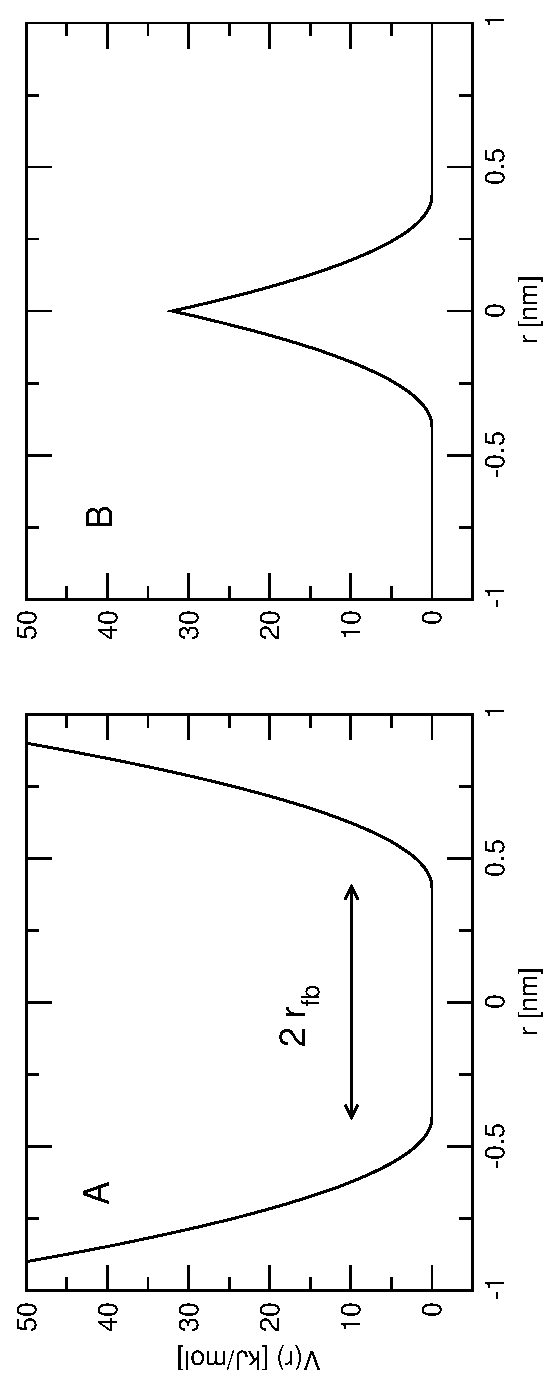
\includegraphics[width=10cm]{plots/fbposres}}
\caption{Flat-bottomed position restraint potential. (A) Not
  inverted, (B) inverted.}
\label{fig:fbposres}
\end{figure}

The following geometries for the flat-bottomed potential are supported:\newline
{\bfseries Sphere} ($g =1$): The particle is kept in a sphere of given
radius. The force acts towards the center of the sphere. The following distance calculation is used:
\beq
  d_g(\ve{r}_i;\ve{R}_i) = |\ve{r}_i-\ve{R}_i|
\eeq
{\bfseries Cylinder} ($g=2$): The particle is kept in a cylinder of given radius
parallel to the $z$-axis. The force from the flat-bottomed potential acts
towards the axis of the cylinder. The $z$-component of the force is zero.
\beq
 d_g(\ve{r}_i;\ve{R}_i) = \sqrt{ (x_i-X_i)^2 + (y_i - Y_i)^2 }
\eeq
{\bfseries Layer} ($g=3,4,5$): The particle is kept in a layer defined by the
thickness and the normal of the layer. The layer normal can be parallel to the $x$, $y$, or
$z$-axis. The force acts parallel to the layer normal.\\
\beq
 d_g(\ve{r}_i;\ve{R}_i) = |x_i-X_i|, \;\;\;\mbox{or}\;\;\; 
 d_g(\ve{r}_i;\ve{R}_i) = |y_i-Y_i|, \;\;\;\mbox{or}\;\;\; 
d_g(\ve{r}_i;\ve{R}_i) = |z_i-Z_i|.
\eeq

It is possible to apply multiple independent flat-bottomed position
restraints of different geometry on one particle. For example, applying
a cylinder and a layer in $z$ keeps a particle within a
disk. Applying three layers in $x$, $y$, and $z$ keeps the particle within a cuboid.

In addition, it is possible to invert the restrained region with the
unrestrained region, leading to a potential that acts to keep the particle {\it outside} of the volume
defined by $\ve{R}_i$, $g$, and $r_\mathrm{fb}$. That feature is
switched on by defining a negative $r_\mathrm{fb}$ in the
topology. The following potential is used (Figure~\ref{fig:fbposres}B):
\beq
  V_\mathrm{fb}^{\mathrm{inv}}(\ve{r}_i) = \frac{1}{2}k_\mathrm{fb}
  [d_g(\ve{r}_i;\ve{R}_i) - |r_\mathrm{fb}|]^2\,
  H[ -(d_g(\ve{r}_i;\ve{R}_i) - |r_\mathrm{fb}|)].
\eeq



%\ifthenelse{\equal{\gmxlite}{1}}{}{
\subsection{Angle restraints\swapindexquiet{angle}{restraint}}
\label{subsec:anglerestraint}
These are used to restrain the angle between two pairs of particles
or between one pair of particles and the $z$-axis.
The functional form is similar to that of a proper dihedral.
For two pairs of atoms: 
\beq
V_{ar}(\ve{r}_i,\ve{r}_j,\ve{r}_k,\ve{r}_l)
        = k_{ar}(1 - \cos(n (\theta - \theta_0))
        )
,~~~~\mbox{where}~~
\theta = \arccos\left(\frac{\ve{r}_j -\ve{r}_i}{\|\ve{r}_j -\ve{r}_i\|}
 \cdot \frac{\ve{r}_l -\ve{r}_k}{\|\ve{r}_l -\ve{r}_k\|} \right)
\eeq
For one pair of atoms and the $z$-axis: 
\beq
V_{ar}(\ve{r}_i,\ve{r}_j) = k_{ar}(1 - \cos(n (\theta - \theta_0))
        )
,~~~~\mbox{where}~~
\theta = \arccos\left(\frac{\ve{r}_j -\ve{r}_i}{\|\ve{r}_j -\ve{r}_i\|}
 \cdot \left( \begin{array}{c} 0 \\ 0 \\ 1 \\ \end{array} \right) \right)
\eeq
A multiplicity ($n$) of 2 is useful when you do not want to distinguish
between parallel and anti-parallel vectors.
The equilibrium angle $\theta$ should be between 0 and 180 degrees
for multiplicity 1 and between 0 and 90 degrees for multiplicity 2.


\subsection{Dihedral restraints\swapindexquiet{dihedral}{restraint}}
\label{subsec:dihedralrestraint}
These are used to restrain the dihedral angle $\phi$ defined by four particles
as in an improper dihedral (sec.~\ref{sec:imp}) but with a slightly
modified potential. Using:
\beq
\phi' = \left(\phi-\phi_0\right) ~{\rm MOD}~ 2\pi
\label{eqn:dphi}
\eeq
where $\phi_0$ is the reference angle, the potential is defined as:
\beq
V_{dihr}(\phi') ~=~ \left\{
\begin{array}{lcllll}
\half k_{dihr}(\phi'-\phi_0-\Delta\phi)^2      
                &\mbox{for}&     \phi' & >   & \Delta\phi       \\[1.5ex]
0               &\mbox{for}&     \phi' & \le & \Delta\phi       \\[1.5ex]
\end{array}\right.
\label{eqn:dihre}
\eeq
where $\Delta\phi$ is a user defined angle and $k_{dihr}$ is the force 
constant.
{\bf Note} that in the input in topology files, angles are given in degrees and
force constants in kJ/mol/rad$^2$.
%} % Brace matches ifthenelse test for gmxlite

\subsection{Distance restraints\swapindexquiet{distance}{restraint}}
\label{subsec:distancerestraint}
Distance restraints 
add a penalty to the potential when the distance between specified
pairs of atoms exceeds a threshold value. They are normally used to
impose experimental restraints from, for instance, experiments in nuclear
magnetic resonance (NMR), on the motion of the system. Thus, MD can be
used for structure refinement using NMR data\index{nmr
refinement}\index{refinement,nmr}.
In {\gromacs} there are three ways to impose restraints on pairs of atoms:
\begin{itemize}
\item Simple harmonic restraints: use {\tt [ bonds ]} type 6
%\ifthenelse{\equal{\gmxlite}{1}}
{.}
{(see \secref{excl}).}
\item\label{subsec:harmonicrestraint}Piecewise linear/harmonic restraints: {\tt [ bonds ]} type 10.
\item Complex NMR distance restraints, optionally with pair, time and/or
ensemble averaging.
\end{itemize}
The last two options will be detailed now.

The potential form for distance restraints is quadratic below a specified
lower bound and between two specified upper bounds, and linear beyond the
largest bound (see \figref{dist}).
\beq
V_{dr}(r_{ij}) ~=~ \left\{
\begin{array}{lcllllll}
\half k_{dr}(r_{ij}-r_0)^2      
                &\mbox{for}&     &     & r_{ij} & < & r_0       \\[1.5ex]
0               &\mbox{for}& r_0 & \le & r_{ij} & < & r_1       \\[1.5ex]
\half k_{dr}(r_{ij}-r_1)^2      
                &\mbox{for}& r_1 & \le & r_{ij} & < & r_2       \\[1.5ex]
\half k_{dr}(r_2-r_1)(2r_{ij}-r_2-r_1)  
                &\mbox{for}& r_2 & \le & r_{ij} &   &
\end{array}\right.
\label{eqn:disre}
\eeq

\begin{figure}
\centerline{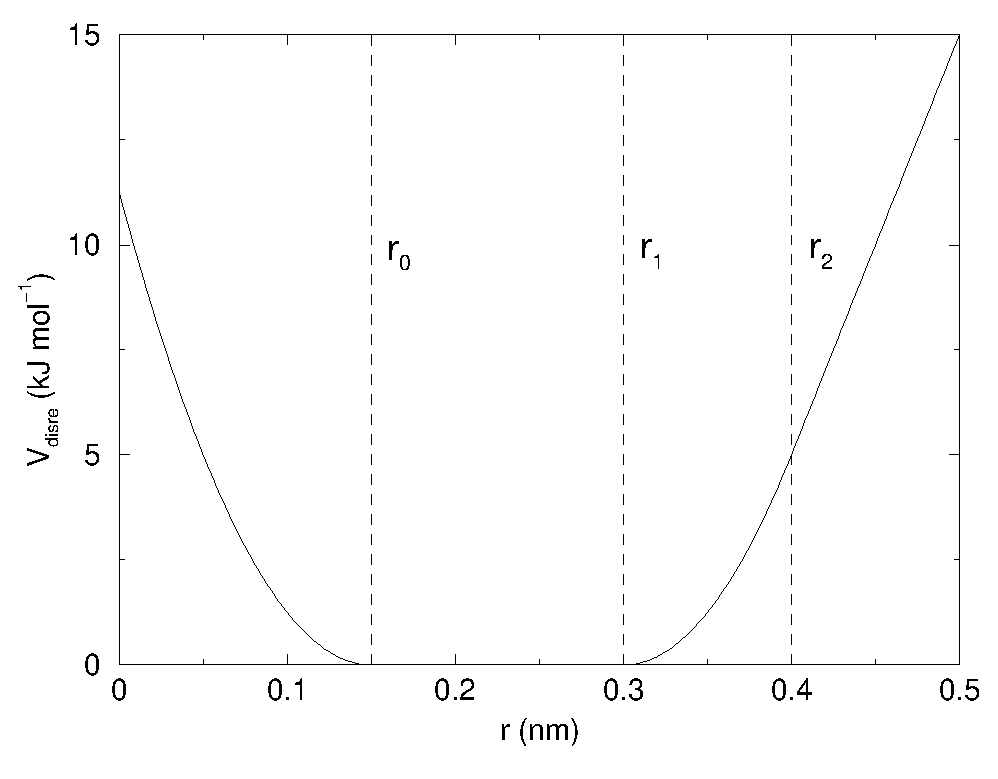
\includegraphics[width=8cm]{plots/f-dr}}
\caption{Distance Restraint potential.}
\label{fig:dist}
\end{figure}

The forces are
\beq
\ve{F}_i~=~ \left\{
\begin{array}{lcllllll}
-k_{dr}(r_{ij}-r_0)\frac{\rvij}{r_{ij}} 
                &\mbox{for}&     &     & r_{ij} & < & r_0       \\[1.5ex]
0               &\mbox{for}& r_0 & \le & r_{ij} & < & r_1       \\[1.5ex]
-k_{dr}(r_{ij}-r_1)\frac{\rvij}{r_{ij}} 
                &\mbox{for}& r_1 & \le & r_{ij} & < & r_2       \\[1.5ex]
-k_{dr}(r_2-r_1)\frac{\rvij}{r_{ij}}    
                &\mbox{for}& r_2 & \le & r_{ij} &   &
\end{array} \right.
\eeq

For restraints not derived from NMR data, this functionality
will usually suffice and a section of {\tt [ bonds ]} type 10
can be used to apply individual restraints between pairs of
%\ifthenelse{\equal{\gmxlite}{1}}{atoms.}{
atoms, see \ssecref{topfile}.
%} % Brace matches ifthenelse test for gmxlite 
For applying restraints derived from NMR measurements, more complex
functionality might be required, which is provided through
the {\tt [~distance_restraints~]} section and is described below.

%\ifthenelse{\equal{\gmxlite}{1}}{}{
\subsubsection{Time averaging\swapindexquiet{time-averaged}{distance restraint}}
Distance restraints based on instantaneous distances can potentially reduce
the fluctuations in a molecule significantly. This problem can be overcome by restraining
to a {\em time averaged} distance~\cite{Torda89}.
The forces with time averaging are:
\beq
\ve{F}_i~=~ \left\{
\begin{array}{lcllllll}
-k^a_{dr}(\bar{r}_{ij}-r_0)\frac{\rvij}{r_{ij}}   
                &\mbox{for}&     &     & \bar{r}_{ij} & < & r_0 \\[1.5ex]
0               &\mbox{for}& r_0 & \le & \bar{r}_{ij} & < & r_1 \\[1.5ex]
-k^a_{dr}(\bar{r}_{ij}-r_1)\frac{\rvij}{r_{ij}}   
                &\mbox{for}& r_1 & \le & \bar{r}_{ij} & < & r_2 \\[1.5ex]
-k^a_{dr}(r_2-r_1)\frac{\rvij}{r_{ij}}    
                &\mbox{for}& r_2 & \le & \bar{r}_{ij} &   &
\end{array} \right.
\eeq
where $\bar{r}_{ij}$ is given by an exponential running average with decay time $\tau$:
\beq
\bar{r}_{ij} ~=~ < r_{ij}^{-3} >^{-1/3}
\label{eqn:rav}
\eeq
The force constant $k^a_{dr}$ is switched on slowly to compensate for
the lack of history at the beginning of the simulation:
\beq
k^a_{dr} = k_{dr} \left(1-\exp\left(-\frac{t}{\tau}\right)\right)
\eeq
Because of the time averaging, we can no longer speak of a distance restraint
potential.

This way an atom can satisfy two incompatible distance restraints 
{\em on average} by moving between two positions. 
An example would be an amino acid side-chain that is rotating around
its $\chi$ dihedral angle, thereby coming close to various other groups.
Such a mobile side chain can give rise to multiple NOEs that can not be
fulfilled by a single structure.

The computation of the time
averaged distance in the {\tt mdrun} program is done in the following fashion:
\beq
\begin{array}{rcl}
\overline{r^{-3}}_{ij}(0)       &=& r_{ij}(0)^{-3}      \\
\overline{r^{-3}}_{ij}(t)       &=& \overline{r^{-3}}_{ij}(t-\Delta t)~\exp{\left(-\frac{\Delta t}{\tau}\right)} + r_{ij}(t)^{-3}\left[1-\exp{\left(-\frac{\Delta t}{\tau}\right)}\right]
\label{eqn:ravdisre}
\end{array}
\eeq

When a pair is within the bounds, it can still feel a force
because the time averaged distance can still be beyond a bound.
To prevent the protons from being pulled too close together, a mixed
approach can be used. In this approach, the penalty is zero when the
instantaneous distance is within the bounds, otherwise the violation is
the square root of the product of the instantaneous violation and the 
time averaged violation:
\beq
\ve{F}_i~=~ \left\{
\begin{array}{lclll}
k^a_{dr}\sqrt{(r_{ij}-r_0)(\bar{r}_{ij}-r_0)}\frac{\rvij}{r_{ij}}   
    & \mbox{for} & r_{ij} < r_0 & \mbox{and} & \bar{r}_{ij} < r_0 \\[1.5ex]
-k^a _{dr} \,
  \mbox{min}\left(\sqrt{(r_{ij}-r_1)(\bar{r}_{ij}-r_1)},r_2-r_1\right)
  \frac{\rvij}{r_{ij}}   
    & \mbox{for} & r_{ij} > r_1 & \mbox{and} & \bar{r}_{ij} > r_1 \\[1.5ex]
0               &\mbox{otherwise}
\end{array} \right.
\eeq

\subsubsection{Averaging over multiple pairs\swapindexquiet{ensemble-averaged}{distance restraint}} 

Sometimes it is unclear from experimental data which atom pair
gives rise to a single NOE, in other occasions it can be obvious that
more than one pair contributes due to the symmetry of the system, {\eg} a
methyl group with three protons. For such a group, it is not possible 
to distinguish between the protons, therefore they should all be taken into
account when calculating the distance between this methyl group and another
proton (or group of protons).
Due to the physical nature of magnetic resonance, the intensity of the
NOE signal is inversely proportional to the sixth power of the inter-atomic 
distance.
Thus, when combining atom pairs, 
a fixed list of $N$ restraints may be taken together, 
where the apparent ``distance'' is given by:
\beq
r_N(t) = \left [\sum_{n=1}^{N} \bar{r}_{n}(t)^{-6} \right]^{-1/6}
\label{eqn:rsix}
\eeq
where we use $r_{ij}$ or \eqnref{rav} for the $\bar{r}_{n}$.
The $r_N$ of the instantaneous and time-averaged distances
can be combined to do a mixed restraining, as indicated above.
As more pairs of protons contribute to the same NOE signal, the intensity
will increase, and the summed ``distance'' will be shorter than any of
its components due to the reciprocal summation. 

There are two options for distributing the forces over the atom pairs.
In the conservative option, the force is defined as the derivative of the
restraint potential with respect to the coordinates. This results in
a conservative potential when time averaging is not used.
The force distribution over the pairs is proportional to $r^{-6}$.
This means that a close pair feels a much larger force than a distant pair,
which might lead to a molecule that is ``too rigid.''
The other option is an equal force distribution. In this case each pair
feels $1/N$ of the derivative of the restraint potential with respect to 
$r_N$. The advantage of this method is that more conformations might be
sampled, but the non-conservative nature of the forces can lead to
local heating of the protons.

It is also possible to use {\em ensemble averaging} using multiple
(protein)  molecules. In this case the bounds should be lowered as in:
\beq
\begin{array}{rcl}
r_1     &~=~&   r_1 * M^{-1/6}  \\
r_2     &~=~&   r_2 * M^{-1/6}
\end{array}
\eeq
where $M$ is the number of molecules. The {\gromacs} preprocessor {\tt grompp}
can do this automatically when the appropriate option is given.
The resulting ``distance'' is 
then used to calculate the scalar force according to:
\beq
\ve{F}_i~=~\left\{
\begin{array}{rcl}
~& 0 \hspace{4cm}  & r_{N} < r_1         \\
 & k_{dr}(r_{N}-r_1)\frac{\rvij}{r_{ij}} & r_1 \le r_{N} < r_2 \\
 & k_{dr}(r_2-r_1)\frac{\rvij}{r_{ij}}    & r_{N} \ge r_2 
\end{array} \right.
\eeq
where $i$ and $j$ denote the atoms of all the 
pairs that contribute to the NOE signal.

\subsubsection{Using distance restraints}

A list of distance restrains based on NOE data can be added to a molecule
definition in your topology file, like in the following example:

\begin{verbatim}
[ distance_restraints ]
; ai   aj   type   index   type'      low     up1     up2     fac
10     16      1       0       1      0.0     0.3     0.4     1.0
10     28      1       1       1      0.0     0.3     0.4     1.0
10     46      1       1       1      0.0     0.3     0.4     1.0
16     22      1       2       1      0.0     0.3     0.4     2.5
16     34      1       3       1      0.0     0.5     0.6     1.0
\end{verbatim}

In this example a number of features can be found.  In columns {\tt
ai} and {\tt aj} you find the atom numbers of the particles to be
restrained. The {\tt type} column should always be 1.  As explained in
~\ssecref{distancerestraint}, multiple distances can contribute to a single NOE
signal. In the topology this can be set using the {\tt index}
column. In our example, the restraints 10-28 and 10-46 both have index
1, therefore they are treated simultaneously.  An extra requirement
for treating restraints together is that the restraints must be on
successive lines, without any other intervening restraint.  The {\tt
type'} column will usually be 1, but can be set to 2 to obtain a
distance restraint that will never be time- and ensemble-averaged;
this can be useful for restraining hydrogen bonds.  The columns {\tt
low}, {\tt up1}, and {\tt up2} hold the values of $r_0$, $r_1$, and
$r_2$ from ~\eqnref{disre}.  In some cases it can be useful to have
different force constants for some restraints; this is controlled by
the column {\tt fac}.  The force constant in the parameter file is
multiplied by the value in the column {\tt fac} for each restraint.
%} % Brace matches ifthenelse test for gmxlite

\newcommand{\SSS}{{\mathbf S}}
\newcommand{\DD}{{\mathbf D}}
\newcommand{\RR}{{\mathbf R}}

%\ifthenelse{\equal{\gmxlite}{1}}{}{
\subsection{Orientation restraints\swapindexquiet{orientation}{restraint}}
\label{subsec:orientationrestraint}
This section describes how orientations between vectors,
as measured in certain NMR experiments, can be calculated
and restrained in MD simulations.
The presented refinement methodology and a comparison of results
with and without time and ensemble averaging have been
published~\cite{Hess2003}.
\subsubsection{Theory}
In an NMR experiment, orientations of vectors can be measured when a 
molecule does not tumble completely isotropically in the solvent.
Two examples of such orientation measurements are
residual \normindex{dipolar couplings}
(between two nuclei) or chemical shift anisotropies.
An observable for a vector $\ve{r}_i$ can be written as follows:
\beq
\delta_i = \frac{2}{3} \mbox{tr}(\SSS\DD_i)
\eeq
where $\SSS$ is the dimensionless order tensor of the molecule.
The tensor $\DD_i$ is given by:
\beq
\label{orient_def}
\DD_i = \frac{c_i}{\|\ve{r}_i\|^\alpha} \left(
%\begin{array}{lll}
%3 r_x r_x - \ve{r}\cdot\ve{r} & 3 r_x r_y & 3 r_x r_z \\
%3 r_x r_y                     & 3 r_y r_y - \ve{r}\cdot\ve{r} & 3yz \\
%3 r_x r_z                     & 3 r_y r_z & 3 r_z r_z - \ve{r}\cdot\ve{r}
%\end{array} \right)
\begin{array}{lll}
3 x x - 1 & 3 x y     & 3 x z     \\
3 x y     & 3 y y - 1 & 3 y z     \\
3 x z     & 3 y z     & 3 z z - 1 \\
\end{array} \right)
\eeq
\beq
\mbox{with:} \quad 
x=\frac{r_{i,x}}{\|\ve{r}_i\|}, \quad
y=\frac{r_{i,y}}{\|\ve{r}_i\|}, \quad 
z=\frac{r_{i,z}}{\|\ve{r}_i\|}
\eeq
For a dipolar coupling $\ve{r}_i$ is the vector connecting the two
nuclei, $\alpha=3$ and the constant $c_i$ is given by:
\beq
c_i = \frac{\mu_0}{4\pi} \gamma_1^i \gamma_2^i \frac{\hbar}{4\pi}
\eeq
where $\gamma_1^i$ and $\gamma_2^i$ are the gyromagnetic ratios of the
two nuclei.

The order tensor is symmetric and has trace zero. Using a rotation matrix
${\mathbf T}$ it can be transformed into the following form:
\beq
{\mathbf T}^T \SSS {\mathbf T} = s \left( \begin{array}{ccc}
-\frac{1}{2}(1-\eta) & 0                    & 0 \\
0                    & -\frac{1}{2}(1+\eta) & 0 \\
0                    & 0                    & 1
\end{array} \right)
\eeq
where $-1 \leq s \leq 1$ and $0 \leq \eta \leq 1$.
$s$ is called the order parameter and $\eta$ the asymmetry of the
order tensor $\SSS$. When the molecule tumbles isotropically in the
solvent, $s$ is zero, and no orientational effects can be observed
because all $\delta_i$ are zero.

%\newpage

\subsubsection{Calculating orientations in a simulation}
For reasons which are explained below, the $\DD$ matrices are calculated
which respect to a reference orientation of the molecule. The orientation
is defined by a rotation matrix $\RR$, which is needed to least-squares fit
the current coordinates of a selected set of atoms onto
a reference conformation. The reference conformation is the starting
conformation of the simulation. In case of ensemble averaging, which will
be treated later, the structure is taken from the first subsystem.
The calculated $\DD_i^c$ matrix is given by:
\begin{equation}
\label{D_rot}
\DD_i^c(t) = \RR(t) \DD_i(t) \RR^T(t)
\end{equation}
The calculated orientation for vector $i$ is given by:
\beq
\delta^c_i(t) = \frac{2}{3} \mbox{tr}(\SSS(t)\DD_i^c(t))
\eeq
The order tensor $\SSS(t)$ is usually unknown.
A reasonable choice for the order tensor is the tensor
which minimizes the (weighted) mean square difference between the calculated
and the observed orientations:
\begin{equation}
\label{S_msd}
MSD(t) = \left(\sum_{i=1}^N w_i\right)^{-1} \sum_{i=1}^N w_i (\delta_i^c (t) -\delta_i^{exp})^2
\end{equation}
To properly combine different types of measurements, the unit of $w_i$ should
be such that all terms are dimensionless. This means the unit of $w_i$
is the unit of $\delta_i$ to the power $-2$.
{\bf Note} that scaling all $w_i$ with a constant factor does not influence
the order tensor.

\subsubsection{Time averaging}
Since the tensors $\DD_i$ fluctuate rapidly in time, much faster than can
be observed in an experiment, they should be averaged over time in the simulation.
However, in a simulation the time and the number of copies of
a molecule are limited. Usually one can not obtain a converged average
of the $\DD_i$ tensors over all orientations of the molecule.
If one assumes that the average orientations of the $\ve{r}_i$ vectors
within the molecule converge much faster than the tumbling time of
the molecule, the tensor can be averaged in an axis system that 
rotates with the molecule, as expressed by equation~(\ref{D_rot}).
The time-averaged tensors are calculated
using an exponentially decaying memory function:
\beq
\DD^a_i(t) = \frac{\displaystyle
\int_{u=t_0}^t \DD^c_i(u) \exp\left(-\frac{t-u}{\tau}\right)\mbox{d} u
}{\displaystyle
\int_{u=t_0}^t \exp\left(-\frac{t-u}{\tau}\right)\mbox{d} u
}
\eeq
Assuming that the order tensor $\SSS$ fluctuates slower than the
$\DD_i$, the time-averaged orientation can be calculated as:
\beq
\delta_i^a(t) = \frac{2}{3} \mbox{tr}(\SSS(t) \DD_i^a(t))
\eeq
where the order tensor $\SSS(t)$ is calculated using expression~(\ref{S_msd})
with $\delta_i^c(t)$ replaced by $\delta_i^a(t)$.

\subsubsection{Restraining}
The simulated structure can be restrained by applying a force proportional
to the difference between the calculated and the experimental orientations.
When no time averaging is applied, a proper potential can be defined as:
\beq
V = \frac{1}{2} k \sum_{i=1}^N w_i (\delta_i^c (t) -\delta_i^{exp})^2
\eeq
where the unit of $k$ is the unit of energy.
Thus the effective force constant for restraint $i$ is $k w_i$.
The forces are given by minus the gradient of $V$.
The force $\ve{F}\!_i$ working on vector $\ve{r}_i$ is:
\begin{eqnarray*}
\ve{F}\!_i(t) 
& = & - \frac{\mbox{d} V}{\mbox{d}\ve{r}_i} \\
& = & -k w_i (\delta_i^c (t) -\delta_i^{exp}) \frac{\mbox{d} \delta_i (t)}{\mbox{d}\ve{r}_i} \\
& = & -k w_i (\delta_i^c (t) -\delta_i^{exp})
\frac{2 c_i}{\|\ve{r}\|^{2+\alpha}} \left(2 \RR^T \SSS \RR \ve{r}_i - \frac{2+\alpha}{\|\ve{r}\|^2} \mbox{tr}(\RR^T \SSS \RR \ve{r}_i \ve{r}_i^T) \ve{r}_i \right)
\end{eqnarray*}

\subsubsection{Ensemble averaging}
Ensemble averaging can be applied by simulating a system of $M$ subsystems
that each contain an identical set of orientation restraints. The systems only
interact via the orientation restraint potential which is defined as:
\beq
V = M \frac{1}{2} k \sum_{i=1}^N w_i 
\langle \delta_i^c (t) -\delta_i^{exp} \rangle^2
\eeq
The force on vector $\ve{r}_{i,m}$ in subsystem $m$ is given by:
\beq
\ve{F}\!_{i,m}(t) = - \frac{\mbox{d} V}{\mbox{d}\ve{r}_{i,m}} =
-k w_i \langle \delta_i^c (t) -\delta_i^{exp} \rangle \frac{\mbox{d} \delta_{i,m}^c (t)}{\mbox{d}\ve{r}_{i,m}} \\
\eeq 

\subsubsection{Time averaging}
When using time averaging it is not possible to define a potential.
We can still define a quantity that gives a rough idea of the energy
stored in the restraints:
\beq
V = M \frac{1}{2} k^a \sum_{i=1}^N w_i 
\langle \delta_i^a (t) -\delta_i^{exp} \rangle^2
\eeq
The force constant $k_a$ is switched on slowly to compensate for the
lack of history at times close to $t_0$. It is exactly proportional
to the amount of average that has been accumulated:
\beq
k^a =
 k \, \frac{1}{\tau}\int_{u=t_0}^t \exp\left(-\frac{t-u}{\tau}\right)\mbox{d} u
\eeq
What really matters is the definition of the force. It is chosen to
be proportional to the square root of the product of the time-averaged
and the instantaneous deviation.
Using only the time-averaged deviation induces large oscillations.
The force is given by:
\beq
\ve{F}\!_{i,m}(t) =
%\left\{ \begin{array}{ll}
%0 & \mbox{for} \quad \langle \delta_i^a (t) -\delta_i^{exp} \rangle \langle \delta_i (t) -\delta_i^{exp} \rangle \leq 0 \\
%... & \mbox{for} \quad \langle \delta_i^a (t) -\delta_i^{exp} \rangle \langle \delta_i (t) -\delta_i^{exp} \rangle > 0 
%\end{array}
%\right.
\left\{ \begin{array}{ll}
0 & \quad \mbox{for} \quad a\, b \leq 0 \\
\displaystyle
k^a w_i \frac{a}{|a|} \sqrt{a\, b} \, \frac{\mbox{d} \delta_{i,m}^c (t)}{\mbox{d}\ve{r}_{i,m}}
& \quad \mbox{for} \quad a\, b > 0 
\end{array}
\right.
\eeq
\begin{eqnarray*}
a &=& \langle \delta_i^a (t) -\delta_i^{exp} \rangle \\
b &=& \langle \delta_i^c (t) -\delta_i^{exp} \rangle
\end{eqnarray*}

\subsubsection{Using orientation restraints}
Orientation restraints can be added to a molecule definition in
the topology file in the section {\tt [~orientation_restraints~]}.
Here we give an example section containing five N-H residual dipolar
coupling restraints:

\begin{verbatim}
[ orientation_restraints ]
; ai   aj  type  exp.  label  alpha    const.     obs.   weight
;                                Hz      nm^3       Hz    Hz^-2
  31   32     1     1      3      3     6.083    -6.73      1.0
  43   44     1     1      4      3     6.083    -7.87      1.0
  55   56     1     1      5      3     6.083    -7.13      1.0
  65   66     1     1      6      3     6.083    -2.57      1.0
  73   74     1     1      7      3     6.083    -2.10      1.0
\end{verbatim}

The unit of the observable is Hz, but one can choose any other unit.
In columns {\tt
ai} and {\tt aj} you find the atom numbers of the particles to be
restrained. The {\tt type} column should always be 1.
The {\tt exp.} column denotes the experiment number, starting
at 1. For each experiment a separate order tensor $\SSS$
is optimized. The label should be a unique number larger than zero
for each restraint. The {\tt alpha} column contains the power $\alpha$ 
that is used in equation~(\ref{orient_def}) to calculate the orientation.
The {\tt const.} column contains the constant $c_i$ used in the same
equation. The constant should have the unit of the observable times
nm$^\alpha$. The column {\tt obs.} contains the observable, in any
unit you like. The last column contains the weights $w_i$; the unit
should be the inverse of the square of the unit of the observable.

Some parameters for orientation restraints can be specified in the
{\tt grompp.mdp} file, for a study of the effect of different
force constants and averaging times and ensemble averaging see~\cite{Hess2003}.
%} % Brace matches ifthenelse test for gmxlite

%\ifthenelse{\equal{\gmxlite}{1}}{}{
\section{Polarization}
Polarization can be treated by {\gromacs} by attaching
\normindex{shell} (\normindex{Drude}) particles to atoms and/or
virtual sites. The energy of the shell particle is then minimized at
each time step in order to remain on the Born-Oppenheimer surface.

\subsection{Simple polarization}
This is merely a harmonic potential with equilibrium distance 0.

\subsection{Water polarization}
A special potential for water that allows anisotropic polarization of
a single shell particle~\cite{Maaren2001a}.

\subsection{Thole polarization}
Based on early work by \normindex{Thole}~\cite{Thole81}, Roux and
coworkers have implemented potentials for molecules like
ethanol~\cite{Lamoureux2003a,Lamoureux2003b,Noskov2005a}. Within such
molecules, there are intra-molecular interactions between shell
particles, however these must be screened because full Coulomb would
be too strong. The potential between two shell particles $i$ and $j$ is:
\newcommand{\rbij}{\bar{r}_{ij}}
\beq
V_{thole} ~=~ \frac{q_i q_j}{r_{ij}}\left[1-\left(1+\frac{\rbij}{2}\right){\rm exp}^{-\rbij}\right]
\eeq
{\bf Note} that there is a sign error in Equation~1 of Noskov {\em et al.}~\cite{Noskov2005a}:
\beq
\rbij ~=~ a\frac{r_{ij}}{(\alpha_i \alpha_j)^{1/6}}
\eeq
where $a$ is a magic (dimensionless) constant, usually chosen to be
2.6~\cite{Noskov2005a}; $\alpha_i$ and $\alpha_j$ are the polarizabilities
of the respective shell particles.

%} % Brace matches ifthenelse test for gmxlite

%\ifthenelse{\equal{\gmxlite}{1}}{}{
\section{Free energy interactions}
\label{sec:feia}
\index{free energy interactions}
\newcommand{\LAM}{\lambda}
\newcommand{\LL}{(1-\LAM)}
\newcommand{\dvdl}[1]{\frac{\partial #1}{\partial \LAM}}
This section describes the $\lambda$-dependence of the potentials
used for free energy calculations (see \secref{fecalc}).
All common types of potentials and constraints can be
interpolated smoothly from state A ($\lambda=0$) to state B
($\lambda=1$) and vice versa.
All bonded interactions are interpolated by linear interpolation
of the interaction parameters. Non-bonded interactions can be
interpolated linearly or via soft-core interactions.

Starting in {\gromacs} 4.6, $\lambda$ is a vector, allowing different
components of the free energy transformation to be carried out at
different rates.  Coulomb, Lennard-Jones, bonded, and restraint terms
can all be controlled independently, as described in the {\tt .mdp}
options.

\subsubsection{Harmonic potentials}
The example given here is for the bond potential, which is harmonic
in {\gromacs}. However,  these equations apply to the angle potential
and the improper dihedral potential as well.
\bea
V_b     &=&\half\left[\LL k_b^A + 
                \LAM k_b^B\right] \left[b - \LL b_0^A - \LAM b_0^B\right]^2  \\
\dvdl{V_b}&=&\half(k_b^B-k_b^A)
                \left[b - \LL b_0^A + \LAM b_0^B\right]^2 + 
		\nonumber\\
        & & \phantom{\half}(b_0^A-b_0^B) \left[b - \LL b_0^A -\LAM b_0^B\right]
		\left[\LL k_b^A + \LAM k_b^B \right]
\eea

\subsubsection{\gromosv{96} bonds and angles}
Fourth-power bond stretching and cosine-based angle potentials
are interpolated by linear interpolation of the force constant
and the equilibrium position. Formulas are not given here.

\subsubsection{Proper dihedrals}
For the proper dihedrals, the equations are somewhat more complicated:
\bea
V_d     &=&\left[\LL k_d^A + \LAM k_d^B \right]
        \left( 1+ \cos\left[n_{\phi} \phi - 
		    \LL \phi_s^A - \LAM \phi_s^B
		    \right]\right)\\
\dvdl{V_d}&=&(k_d^B-k_d^A) 
         \left( 1+ \cos
		 \left[
		    n_{\phi} \phi- \LL \phi_s^A - \LAM \phi_s^B
		 \right]
	 \right) +
	 \nonumber\\
        &&(\phi_s^B - \phi_s^A) \left[\LL k_d^A - \LAM k_d^B\right] 
        \sin\left[  n_{\phi}\phi - \LL \phi_s^A - \LAM \phi_s^B \right]
\eea
{\bf Note:} that the multiplicity $n_{\phi}$ can not be parameterized
because the function should remain periodic on the interval $[0,2\pi]$.

\subsubsection{Tabulated bonded interactions}
For tabulated bonded interactions only the force constant can interpolated:
\bea
      V  &=& (\LL k^A + \LAM k^B) \, f \\
\dvdl{V} &=& (k^B - k^A) \, f
\eea

\subsubsection{Coulomb interaction}
The \normindex{Coulomb} interaction between two particles 
of which the charge varies with $\LAM$ is:
\bea
V_c &=& \frac{f}{\epsrf \rij}\left[\LL q_i^A q_j^A + \LAM\, q_i^B q_j^B\right] \\
\dvdl{V_c}&=& \frac{f}{\epsrf \rij}\left[- q_i^A q_j^A + q_i^B q_j^B\right]
\eea
where $f = \frac{1}{4\pi \varepsilon_0} = 138.935\,485$ (see \chref{defunits}).

\subsubsection{Coulomb interaction with \normindex{reaction field}}
The Coulomb interaction including a reaction field, between two particles 
of which the charge varies with $\LAM$ is:
\bea
V_c     &=& f\left[\frac{1}{\rij} + k_{rf}~ \rij^2 -c_{rf}\right]
             \left[\LL q_i^A q_j^A + \LAM\, q_i^B q_j^B\right] \\
\dvdl{V_c}&=& f\left[\frac{1}{\rij} + k_{rf}~ \rij^2 -c_{rf}\right]
               \left[- q_i^A q_j^A + q_i^B q_j^B\right]
	       \label{eq:dVcoulombdlambda}
\eea
{\bf Note} that the constants $k_{rf}$ and $c_{rf}$ are 
defined using the dielectric 
constant $\epsrf$ of the medium (see \secref{coulrf}).

\subsubsection{Lennard-Jones interaction}
For the \normindex{Lennard-Jones} interaction between two particles 
of which the {\em atom type} varies with $\LAM$ we can write:
\bea
V_{LJ}  &=&     \frac{\LL C_{12}^A + \LAM\, C_{12}^B}{\rij^{12}} -
                \frac{\LL C_6^A + \LAM\, C_6^B}{\rij^6}   \\
\dvdl{V_{LJ}}&=&\frac{C_{12}^B - C_{12}^A}{\rij^{12}} -
                \frac{C_6^B - C_6^A}{\rij^6}
		\label{eq:dVljdlambda}
\eea
It should be noted that it is also possible to express a pathway from
state A to state B using $\sigma$ and $\epsilon$ (see \eqnref{sigeps}).
It may seem to make sense physically to vary the force field parameters
$\sigma$ and $\epsilon$ rather 
than the derived parameters $C_{12}$ and $C_{6}$.
However, the difference between the pathways in parameter space
is not large, and the free energy itself
does not depend on the pathway, so we use the simple formulation
presented above.

\subsubsection{Kinetic Energy}
When the mass of a particle changes, there is also a contribution of
the kinetic energy to the free energy (note that we can not write 
the momentum \ve{p} as m\ve{v}, since that would result 
in the sign of $\dvdl{E_k}$ being incorrect~\cite{Gunsteren98a}):

\bea
E_k      &=&     \half\frac{\ve{p}^2}{\LL m^A + \LAM m^B}        \\
\dvdl{E_k}&=&    -\half\frac{\ve{p}^2(m^B-m^A)}{(\LL m^A + \LAM m^B)^2}
\eea
after taking the derivative, we {\em can} insert \ve{p} = m\ve{v}, such that:
\beq
\dvdl{E_k}~=~    -\half\ve{v}^2(m^B-m^A)
\eeq

\subsubsection{Constraints}
\label{subsubsec:constraints}
\newcommand{\clam}{C_{\lambda}}
The constraints are formally part of the Hamiltonian, and therefore
they give a contribution to the free energy. In {\gromacs} this can be
calculated using the \normindex{LINCS} or the \normindex{SHAKE} algorithm.
If we have a number of constraint equations $g_k$:
\beq
g_k     =       \ve{r}_{k} - d_{k}
\eeq
where $\ve{r}_k$ is the distance vector between two particles and 
$d_k$ is the constraint distance between the two particles, we can write
this using a $\LAM$-dependent distance as
\beq
g_k     =       \ve{r}_{k} - \left(\LL d_{k}^A + \LAM d_k^B\right)
\eeq
the contribution $\clam$ 
to the Hamiltonian using Lagrange multipliers $\lambda$:
\bea
\clam           &=&     \sum_k \lambda_k g_k    \\
\dvdl{\clam}    &=&     \sum_k \lambda_k \left(d_k^B-d_k^A\right)
\eea


\subsection{Soft-core interactions\index{soft-core interactions}}
\begin{figure}
\centerline{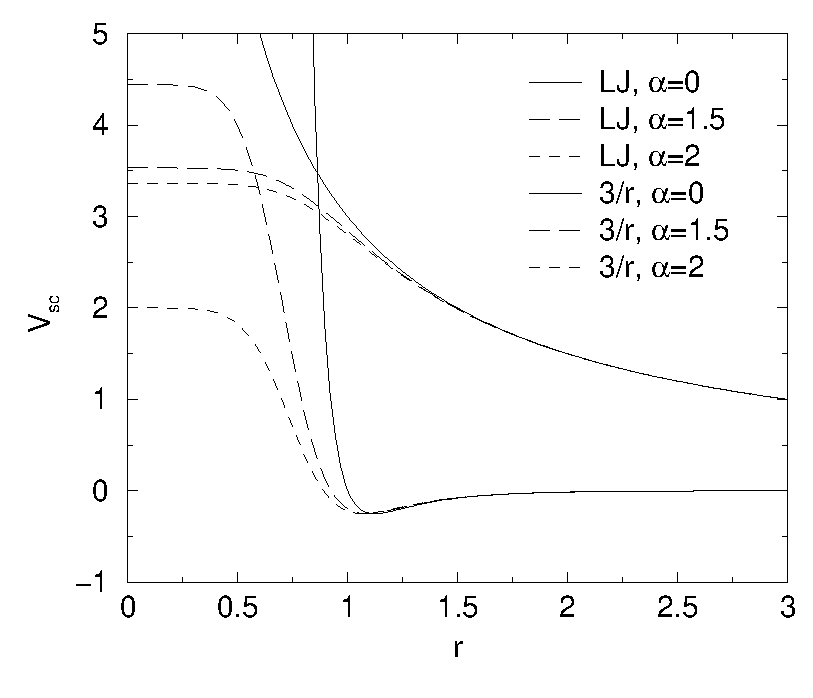
\includegraphics[height=6cm]{plots/softcore}}
\caption{Soft-core interactions at $\LAM=0.5$, with $p=2$ and
$C_6^A=C_{12}^A=C_6^B=C_{12}^B=1$.}
\label{fig:softcore}
\end{figure}
In a free-energy calculation where particles grow out of nothing, or 
particles disappear, using the the simple linear interpolation of the 
Lennard-Jones and Coulomb potentials as described in Equations~\ref{eq:dVljdlambda}
and \ref{eq:dVcoulombdlambda} may lead to poor convergence.  When the particles have nearly disappeared, or are close to appearing (at $\LAM$ close to 0 or 1), the interaction energy will be weak enough for particles to get very 
close to each other, leading to large fluctuations in the measured values of 
$\partial V/\partial \LAM$ (which, because of the simple linear 
interpolation, depends on the potentials at both the endpoints of $\LAM$).

To circumvent these problems, the singularities in the potentials need to be removed. This can be done by modifying the regular Lennard-Jones and Coulomb potentials with ``soft-core'' potentials that limit the energies and forces 
involved at $\LAM$ values between 0 and 1, but not \emph{at} $\LAM=0$ 
or 1.

In {\gromacs} the soft-core potentials $V_{sc}$ are shifted versions of the
regular potentials, so that the singularity in the potential and its
derivatives at $r=0$ is never reached:
\bea
V_{sc}(r) &=& \LL V^A(r_A) + \LAM V^B(r_B)
    \\
r_A &=& \left(\alpha \sigma_A^6 \LAM^p + r^6 \right)^\frac{1}{6}
    \\
r_B &=& \left(\alpha \sigma_B^6 \LL^p + r^6 \right)^\frac{1}{6}
\eea
where $V^A$ and $V^B$ are the normal ``hard core'' Van der Waals or
electrostatic potentials in state A ($\LAM=0$) and state B ($\LAM=1$)
respectively, $\alpha$ is the soft-core parameter (set with {\tt sc_alpha} 
in the {\tt .mdp} file), $p$ is the soft-core $\LAM$ power (set with 
{\tt sc_power}), $\sigma$ is the radius of the interaction, which is 
$(C_{12}/C_6)^{1/6}$ or an input parameter ({\tt sc_sigma}) when $C_6$ 
or $C_{12}$ is zero.

For intermediate $\LAM$, $r_A$ and $r_B$ alter the interactions very little
for $r > \alpha^{1/6} \sigma$ and quickly switch the soft-core
interaction to an almost constant value for smaller $r$ (\figref{softcore}). 
The force is:
\beq
F_{sc}(r) = -\frac{\partial V_{sc}(r)}{\partial r} =
 \LL F^A(r_A) \left(\frac{r}{r_A}\right)^5 +
\LAM F^B(r_B) \left(\frac{r}{r_B}\right)^5
\eeq
where $F^A$ and $F^B$ are the ``hard core'' forces.
The contribution to the derivative of the free energy is:
\bea
\dvdl{V_{sc}(r)} & = &
 V^B(r_B) -V^A(r_A)  + 
	\LL \frac{\partial V^A(r_A)}{\partial r_A}
		   \frac{\partial r_A}{\partial \LAM} + 
	\LAM\frac{\partial V^B(r_B)}{\partial r_B}
		   \frac{\partial r_B}{\partial \LAM}
\nonumber\\
&=&
 V^B(r_B) -V^A(r_A)  + \nonumber \\
 & &
 \frac{p \alpha}{6}
       \left[ \LAM F^B(r_B) r^{-5}_B \sigma_B^6 \LL^{p-1} -
	       \LL F^A(r_A) r^{-5}_A \sigma_A^6 \LAM^{p-1} \right]
\eea

The original GROMOS Lennard-Jones soft-core function~\cite{Beutler94}
uses $p=2$, but $p=1$ gives a smoother $\partial H/\partial\LAM$ curve.
%When the changes between the two states involve both the disappearing
%and appearing of atoms, it is important that the overlapping of atoms
%happens around $\LAM=0.5$. This can usually be achieved with
%$\alpha$$\approx0.7$ for $p=1$ and $\alpha$$\approx1.5$ for $p=2$.
%MRS: this is now eliminated as of 4.6, since changes between atoms are done linearly.

Another issue that should be considered is the soft-core effect of hydrogens
without Lennard-Jones interaction. Their soft-core $\sigma$ is
set with {\tt sc-sigma} in the {\tt .mdp} file. These hydrogens
produce peaks in $\partial H/\partial\LAM$ at $\LAM$ is 0 and/or 1 for $p=1$
and close to 0 and/or 1 with $p=2$. Lowering {\tt\mbox{sc-sigma}} will decrease
this effect, but it will also increase the interactions with hydrogens
relative to the other interactions in the soft-core state.

When soft core potentials are selected (by setting {\tt sc-alpha} \textgreater
0), and the Coulomb and Lennard-Jones potentials are turned on or off
sequentially, then the Coulombic interaction is turned off linearly,
rather than using soft core interactions, which should be less
statistically noisy in most cases.  This behavior can be overwritten
by using the mdp option {\tt sc-coul} to {\tt yes}. Additionally, the
soft-core interaction potential is only applied when either the A or B
state has zero interaction potential.  If both A and B states have
nonzero interaction potential, default linear scaling described above
is used. When both Coulombic and Lennard-Jones interactions are turned
off simultaneously, a soft-core potential is used, and a hydrogen is
being introduced or deleted, the sigma is set to {\tt sc-sigma-min},
which itself defaults to {\tt sc-sigma-default}.

Recently, a new formulation of the soft-core approach has been derived
that in most cases gives lower and more even statistical variance than
the standard soft-core path described above.~\cite{Pham2011,Pham2012}
Specifically, we have:
\bea
V_{sc}(r) &=& \LL V^A(r_A) + \LAM V^B(r_B)
    \\
r_A &=& \left(\alpha \sigma_A^{48} \LAM^p + r^{48} \right)^\frac{1}{48}
    \\
r_B &=& \left(\alpha \sigma_B^{48} \LL^p + r^{48} \right)^\frac{1}{48}
\eea
This ``1-1-48'' path is also implemented in {\gromacs}. Note that for this path the soft core $\alpha$
should satisfy $0.001 < \alpha < 0.003$, rather than $\alpha \approx
0.5$.

%} % Brace matches ifthenelse test for gmxlite

%\ifthenelse{\equal{\gmxlite}{1}}{}{
\section{Methods}
\subsection{Exclusions and 1-4 Interactions.}
Atoms within a molecule that are close by in the chain, 
{\ie} atoms that are covalently bonded, or linked by one or two
atoms are called {\em first neighbors, second neighbors} and 
{\em \swapindex{third}{neighbor}s}, respectively (see \figref{chain}).  
Since the interactions of atom {\bf i} with atoms {\bf i+1} and {\bf i+2} 
are mainly quantum mechanical, they can not be modeled by a Lennard-Jones potential.
Instead it is assumed that these interactions are adequately modeled
by a harmonic bond term or constraint ({\bf i, i+1}) and a harmonic angle term
({\bf i, i+2}). The first and second neighbors (atoms {\bf i+1} and {\bf i+2}) 
are therefore
{\em excluded} from the Lennard-Jones \swapindex{interaction}{list} 
of atom {\bf i};
atoms {\bf i+1} and {\bf i+2} are called {\em \normindex{exclusions}} of atom {\bf i}.

\begin{figure}
\centerline{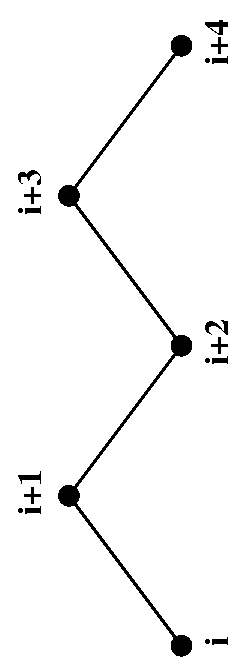
\includegraphics[width=8cm]{plots/chain}}
\caption{Atoms along an alkane chain.}
\label{fig:chain}
\end{figure}

For third neighbors, the normal Lennard-Jones repulsion is sometimes
still too strong, which means that when applied to a molecule, the
molecule would deform or break due to the internal strain. This is
especially the case for carbon-carbon interactions in a {\em
cis}-conformation ({\eg} {\em cis}-butane).  Therefore, for some of these
interactions, the Lennard-Jones repulsion has been reduced in the
{\gromos} force field, which is implemented by keeping a separate list of
1-4 and normal Lennard-Jones parameters. In other force fields, such
as OPLS~\cite{Jorgensen88}, the standard Lennard-Jones parameters are reduced
by a factor of two, but in that case also the dispersion (r$^{-6}$)
and the Coulomb interaction are scaled.
{\gromacs} can use either of these methods.

\subsection{Charge Groups\index{charge group}}
\label{sec:cg}
In principle, the force calculation in MD is an $O(N^2)$ problem.
Therefore, we apply a \normindex{cut-off} for non-bonded force (NBF)
calculations; only the particles within a certain distance of each
other are interacting. This reduces the cost to $O(N)$ (typically
$100N$ to $200N$) of the NBF. It also introduces an error, which is,
in most cases, acceptable, except when applying the cut-off implies
the creation of charges, in which case you should consider using the
lattice sum methods provided by {\gromacs}.

Consider a water molecule interacting with another atom. If we would apply
a plain cut-off on an atom-atom basis we might include the atom-oxygen
interaction (with a charge of $-0.82$) without the compensating charge
of the protons, and as a result, induce a large dipole moment over the system.
Therefore, we have to keep groups of atoms with total charge
0 together. These groups are called {\em charge groups}. Note that with
a proper treatment of long-range electrostatics (e.g. particle-mesh Ewald
(\secref{pme}), keeping charge groups together is not required.

\subsection{Treatment of Cut-offs in the group scheme\index{cut-off}}
\newcommand{\rs}{$r_{short}$}
\newcommand{\rl}{$r_{long}$}
{\gromacs} is quite flexible in treating cut-offs, which implies
there can be quite a number of parameters to set. These parameters are
set in the input file for {\tt grompp}. There are two sort of parameters
that affect the cut-off interactions; you can select which type
of interaction to use in each case, and which cut-offs should be
used in the neighbor searching.

For both Coulomb and van der Waals interactions there are interaction
type selectors (termed {\tt vdwtype} and {\tt coulombtype}) and two
parameters, for a total of six non-bonded interaction parameters. See
\secref{mdpopt} for a complete description of these parameters.

The neighbor searching (NS) can be performed using a single-range, or a twin-range 
approach. Since the former is merely a special case of the latter, we will 
discuss the more general twin-range. In this case, NS is described by two
radii: {\tt rlist} and max({\tt rcoulomb},{\tt rvdw}).
Usually one builds the neighbor list every 10 time steps
or every 20 fs (parameter {\tt nstlist}). In the neighbor list, all interaction 
pairs that  fall within {\tt rlist} are stored. Furthermore, the 
interactions between pairs that do not
fall within {\tt rlist} but do fall within max({\tt rcoulomb},{\tt rvdw})
are computed during NS.  The
forces and energy are stored separately and added to short-range forces
at every time step between successive NS. If {\tt rlist} = 
max({\tt rcoulomb},{\tt rvdw}), no forces
are evaluated during neighbor list generation.
The \normindex{virial} is calculated from the sum of the short- and
long-range forces.
This means that the virial can be slightly asymmetrical at non-NS steps.
When mdrun is compiled to use mixed precision, the virial is almost always asymmetrical because the
off-diagonal elements are about as large as each element in the sum.
In most cases this is not really a problem, since the fluctuations in the
virial can be 2 orders of magnitude larger than the average.

Except for the plain cut-off,
all of the interaction functions in \tabref{funcparm}
require that neighbor searching be done with a larger radius than the $r_c$
specified for the functional form, because of the use of charge groups.
The extra radius is typically of the order of 0.25 nm (roughly the 
largest distance between two atoms in a charge group plus the distance a 
charge group can diffuse within neighbor list updates).

%If your charge groups are very large it may be interesting to turn off charge
%groups, by setting the option 
%{\tt bAtomList = yes} in your {\tt grompp.mdp} file.
%In this case only a small extra radius to account for diffusion needs to be 
%added (0.1 nm). Do not however use this together with the plain cut-off
%method, as it will generate large artifacts (\secref{cg}).
%In summary, there are four parameters that describe NS behavior:
%{\tt nstlist} (update frequency in number of time steps),
%{\tt bAtomList} (whether or not charge groups are used to generate neighbor list, the default is to use charge groups, so {\tt bAtomList = no}),
%{\tt rshort} and {\tt rlong} which are the two radii {\rs} and {\rl}
%described above.

\begin{table}[ht]
\centering
\begin{tabular}{|ll|l|}
\dline
\multicolumn{2}{|c|}{Type}              & Parameters            \\
\hline
Coulomb&Plain cut-off   & $r_c$, $\epsr$        \\
&Reaction field         & $r_c$, $\epsrf$       \\
&Shift function         & $r_1$, $r_c$, $\epsr$         \\
&Switch function        & $r_1$, $r_c$, $\epsr$         \\
\hline
VdW&Plain cut-off       & $r_c$         \\
&Shift function         & $r_1$, $r_c$          \\
&Switch function        & $r_1$, $r_c$          \\
\dline
\end{tabular}
\caption[Parameters for the different functional forms of the
non-bonded interactions.]{Parameters for the different functional
forms of the non-bonded interactions.}
\label{tab:funcparm}
\end{table}
%} % Brace matches ifthenelse test for gmxlite


\newcommand{\vvis}{\ve{r}_s}
\newcommand{\Fi}{\ve{F}_i'}
\newcommand{\Fj}{\ve{F}_j'}
\newcommand{\Fk}{\ve{F}_k'}
\newcommand{\Fl}{\ve{F}_l'}
\newcommand{\Fvis}{\ve{F}_{s}}
\newcommand{\rvik}{\ve{r}_{ik}}
\newcommand{\rvis}{\ve{r}_{is}}
\newcommand{\rvjk}{\ve{r}_{jk}}
\newcommand{\rvjl}{\ve{r}_{jl}}

%\ifthenelse{\equal{\gmxlite}{1}}{}{
\section{Virtual interaction sites\index{virtual interaction sites}}
\label{sec:virtual_sites}
Virtual interaction sites (called \seeindex{dummy atoms}{virtual interaction sites} in {\gromacs} versions before 3.3)
can be used in {\gromacs} in a number of ways. 
We write the position of the virtual site $\ve{r}_s$ as a function of
the positions of other particles \ve{r}$_i$: $\ve{r}_s =
f(\ve{r}_1..\ve{r}_n)$. The virtual site, which may carry charge or be
involved in other interactions, can now be used in the force
calculation.  The force acting on the virtual site must be
redistributed over the particles with mass in a consistent way.
A good way to do this can be found in ref.~\cite{Berendsen84b}.
We can write the potential energy as:
\beq
V = V(\vvis,\ve{r}_1,\ldots,\ve{r}_n) = V^*(\ve{r}_1,\ldots,\ve{r}_n)
\eeq
The force on the particle $i$ is then:
\beq
\ve{F}_i = -\frac{\partial V^*}{\partial \ve{r}_i} 
         = -\frac{\partial V}{\partial \ve{r}_i} - 
            \frac{\partial V}{\partial \vvis} 
            \frac{\partial \vvis}{\partial \ve{r}_i}
         = \ve{F}_i^{direct} + \Fi
\eeq
The first term is the normal force. 
The second term is the force on particle $i$ due to the virtual site, which
can be written in tensor notation:
\newcommand{\partd}[2]{\displaystyle\frac{\partial #1}{\partial #2_i}}
\beq
\Fi = \left[\begin{array}{ccc}
\partd{x_s}{x} & \partd{y_s}{x} & \partd{z_s}{x}        \\[1ex]
\partd{x_s}{y} & \partd{y_s}{y} & \partd{z_s}{y}        \\[1ex]
\partd{x_s}{z} & \partd{y_s}{z} & \partd{z_s}{z}
\end{array}\right]\Fvis
\label{eqn:fvsite}
\eeq
where $\Fvis$ is the force on the virtual site and $x_s$, $y_s$ and
$z_s$ are the coordinates of the virtual site. In this way, the total
force and the total torque are conserved~\cite{Berendsen84b}.

The computation of the \normindex{virial}
(\eqnref{Xi}) is non-trivial when virtual sites are used. Since the
virial involves a summation over all the atoms (rather than virtual
sites), the forces must be redistributed from the virtual sites to the
atoms (using ~\eqnref{fvsite}) {\em before} computation of the
virial. In some special cases where the forces on the atoms can be
written as a linear combination of the forces on the virtual sites (types 2
and 3 below) there is no difference between computing the virial
before and after the redistribution of forces.  However, in the
general case redistribution should be done first.

\begin{figure}
\centerline{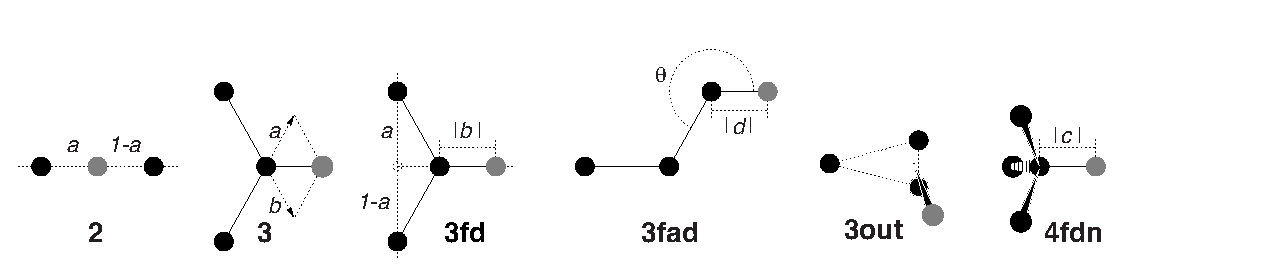
\includegraphics[width=15cm]{plots/dummies}}
\caption[Virtual site construction.]{The six different types of virtual
site construction in \protect{\gromacs}. The constructing atoms are
shown as black circles, the virtual sites in gray.}
\label{fig:vsites}
\end{figure}

There are six ways to construct virtual sites from surrounding atoms in
{\gromacs}, which we classify by the number of constructing
atoms. {\bf Note} that all site types mentioned can be constructed from
types 3fd (normalized, in-plane) and 3out (non-normalized, out of
plane). However, the amount of computation involved increases sharply
along this list, so we strongly recommended using the first adequate
virtual site type that will be sufficient for a certain purpose.
\figref{vsites} depicts 6 of the available virtual site constructions.
The conceptually simplest construction types are linear combinations:
\beq
\vvis = \sum_{i=1}^N w_i \, \ve{r}_i
\eeq
The force is then redistributed using the same weights:
\beq
\Fi = w_i \, \Fvis
\eeq

The types of virtual sites supported in {\gromacs} are given in the list below.
Constructing atoms in virtual sites can be virtual sites themselves, but
only if they are higher in the list, i.e. virtual sites can be
constructed from ``particles'' that are simpler virtual sites.
\begin{itemize}
\item[{\bf\sf 2.}]\label{subsec:vsite2}As a linear combination of two atoms
        (\figref{vsites} 2):
\beq
        w_i = 1 - a ~,~~ w_j = a
\eeq
        In this case the virtual site is on the line through atoms $i$ and
        $j$.

\item[{\bf\sf 3.}]\label{subsec:vsite3}As a linear combination of three atoms
        (\figref{vsites} 3):
\beq
        w_i = 1 - a - b ~,~~ w_j = a ~,~~ w_k = b
\eeq
        In this case the virtual site is in the plane of the other three
	particles.

\item[{\bf\sf 3fd.}]\label{subsec:vsite3fd}In the plane of three atoms, with a fixed distance
        (\figref{vsites} 3fd):
\beq
        \vvis ~=~ \ve{r}_i + b \frac{  \rvij + a \rvjk  }
                                    {| \rvij + a \rvjk |}      
\eeq
        In this case the virtual site is in the plane of the other three
        particles at a distance of $|b|$ from $i$.
        The force on particles $i$, $j$ and $k$ due to the force on the virtual
        site can be computed as:
\beq
        \begin{array}{lcr}
        \Fi &=& \displaystyle \Fvis - \gamma ( \Fvis - \ve{p} ) \\[1ex]
        \Fj &=& \displaystyle (1-a)\gamma (\Fvis - \ve{p})      \\[1ex]
        \Fk &=& \displaystyle a \gamma (\Fvis - \ve{p})         \\
        \end{array}
        ~\mbox{~ where~ }~
        \begin{array}{c}
\displaystyle \gamma = \frac{b}{| \rvij + a \rvjk |} \\[2ex]
\displaystyle \ve{p} = \frac{ \rvis \cdot \Fvis }
                      { \rvis \cdot \rvis } \rvis
        \end{array}
\eeq

\item[{\bf\sf 3fad.}]\label{subsec:vsite3fad}In the plane of three atoms, with a fixed angle and
        distance (\figref{vsites} 3fad):
\beq
\label{eqn:vsite2fad-F}
         \vvis ~=~ \ve{r}_i +
                    d \cos \theta \frac{\rvij}{|\rvij|} +
                    d \sin \theta \frac{\ve{r}_\perp}{|\ve{r}_\perp|}
        ~\mbox{~ where~ }~
        \ve{r}_\perp ~=~ \rvjk - 
                        \frac{ \rvij \cdot \rvjk }
                             { \rvij \cdot \rvij }
                         \rvij
\eeq
        In this case the virtual site is in the plane of the other three
        particles at a distance of $|d|$ from $i$ at an angle of
        $\alpha$ with $\rvij$. Atom $k$ defines the plane and the
        direction of the angle. {\bf Note} that in this case $b$ and
        $\alpha$ must be specified, instead of $a$ and $b$ (see also
        \secref{vsitetop}). The force on particles $i$, $j$ and $k$
        due to the force on the virtual site can be computed as (with
        $\ve{r}_\perp$ as defined in \eqnref{vsite2fad-F}):
\newcommand{\dfrac}{\displaystyle\frac}
\beq
\begin{array}{c}
        \begin{array}{lclllll}
        \Fi &=& \Fvis &-& 
                \dfrac{d \cos \theta}{|\rvij|} \ve{F}_1 &+&
                \dfrac{d \sin \theta}{|\ve{r}_\perp|} \left( 
                \dfrac{ \rvij \cdot \rvjk }
                     { \rvij \cdot \rvij } \ve{F}_2     +
                \ve{F}_3 \right)                                \\[3ex]
        \Fj &=& &&
                \dfrac{d \cos \theta}{|\rvij|} \ve{F}_1 &-&
                \dfrac{d \sin \theta}{|\ve{r}_\perp|} \left(
                 \ve{F}_2 + 
                 \dfrac{ \rvij \cdot \rvjk }
                        { \rvij \cdot \rvij } \ve{F}_2 +
                \ve{F}_3 \right)                                \\[3ex]
        \Fk &=& && &&
                \dfrac{d \sin \theta}{|\ve{r}_\perp|} \ve{F}_2  \\[3ex]
        \end{array}                                             \\[5ex]
        \mbox{where ~}
        \ve{F}_1 = \Fvis -
                  \dfrac{ \rvij \cdot \Fvis }
                        { \rvij \cdot \rvij } \rvij
        \mbox{\,, ~}
        \ve{F}_2 = \ve{F}_1 -
                  \dfrac{ \ve{r}_\perp \cdot \Fvis }
                        { \ve{r}_\perp \cdot \ve{r}_\perp } \ve{r}_\perp
        \mbox{~and ~}
        \ve{F}_3 = \dfrac{ \rvij \cdot \Fvis }
                         { \rvij \cdot \rvij } \ve{r}_\perp
\end{array}
\eeq

\item[{\bf\sf 3out.}]\label{subsec:vsite3out}As a non-linear combination of three atoms, out of plane
        (\figref{vsites} 3out):
\beq
        \vvis ~=~ \ve{r}_i + a \rvij + b \rvik +
                c (\rvij \times \rvik)
\eeq
        This enables the construction of virtual sites out of the plane of the
        other atoms.
        The force on particles $i,j$ and $k$ due to the force on the virtual
        site can be computed as:
\beq
\begin{array}{lcl}
\vspace{4mm}
\Fj &=& \left[\begin{array}{ccc}
 a              &  -c\,z_{ik}   & c\,y_{ik}     \\[0.5ex]
 c\,z_{ik}      &   a           & -c\,x_{ik}    \\[0.5ex]
-c\,y_{ik}      &   c\,x_{ik}   & a
\end{array}\right]\Fvis                                 \\
\vspace{4mm}
\Fk &=& \left[\begin{array}{ccc}
 b              &   c\,z_{ij}   & -c\,y_{ij}    \\[0.5ex]
-c\,z_{ij}      &   b           & c\,x_{ij}     \\[0.5ex]
 c\,y_{ij}      &  -c\,x_{ij}   & b
\end{array}\right]\Fvis                                 \\
\Fi &=& \Fvis - \Fj - \Fk
\end{array}
\eeq

\item[{\bf\sf 4fdn.}]\label{subsec:vsite4fdn}From four atoms, with a fixed distance, see separate Fig.\ \ref{fig:vsite-4fdn}.
This construction is a bit
complex, in particular since the previous type (4fd) could be unstable which forced us
to introduce a more elaborate construction:

\begin{figure}
\centerline{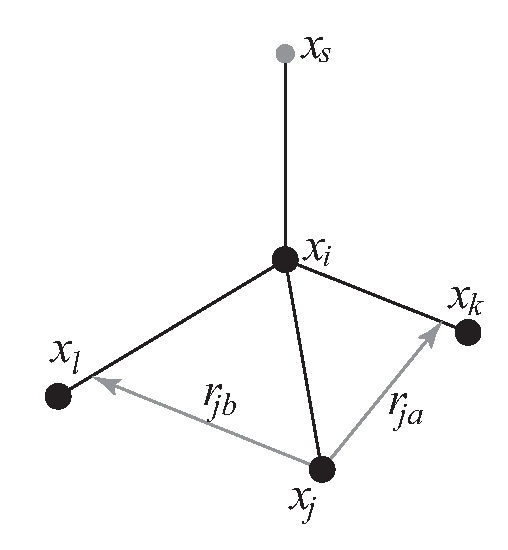
\includegraphics[width=5cm]{plots/vsite-4fdn}}
\caption {The new 4fdn virtual site construction, which is stable even when all constructing
atoms are in the same plane.}
\label{fig:vsite-4fdn}
\end{figure}
         
\begin{eqnarray}
\mathbf{r}_{ja} &=& a\, \mathbf{r}_{ik} - \mathbf{r}_{ij} = a\, (\mathbf{x}_k - \mathbf{x}_i) - (\mathbf{x}_j - \mathbf{x}_i) \nonumber \\
\mathbf{r}_{jb} &=& b\, \mathbf{r}_{il} - \mathbf{r}_{ij} = b\, (\mathbf{x}_l - \mathbf{x}_i) - (\mathbf{x}_j - \mathbf{x}_i) \nonumber \\
\mathbf{r}_m &=& \mathbf{r}_{ja} \times \mathbf{r}_{jb} \nonumber \\
\mathbf{x}_s &=& \mathbf{x}_i + c \frac{\mathbf{r}_m}{|\mathbf{r}_m|}
\label{eq:vsite}
\end{eqnarray}

        In this case the virtual site is at a distance of $|c|$ from $i$, while $a$ and $b$ are 
        parameters. {\bf Note} that the vectors $\mathbf{r}_{ik}$ and $\mathbf{r}_{ij}$ are not normalized
        to save floating-point operations.
        The force on particles $i$, $j$, $k$ and $l$ due to the force 
        on the virtual site are computed through chain rule derivatives
        of the construction expression. This is exact and conserves energy,
        but it does lead to relatively lengthy expressions that we do not
        include here (over 200 floating-point operations). The interested reader can 
        look at the source code in \verb+vsite.c+. Fortunately, this vsite type is normally
        only used for chiral centers such as $C_{\alpha}$ atoms in proteins.
      
The new 4fdn construct is identified with a `type' value of 2 in the topology. The earlier 4fd
type is still supported internally (`type' value 1), but it should not be used for
new simulations. All current {\gromacs} tools will automatically generate type 4fdn instead.


\item[{\bf\sf N.}]\label{subsec:vsiteN} A linear combination of $N$ atoms with relative
weights $a_i$. The weight for atom $i$ is:
\beq
  w_i = a_i \left(\sum_{j=1}^N a_j \right)^{-1}
\eeq
There are three options for setting the weights:
\begin{itemize}
\item[COG] center of geometry: equal weights
\item[COM] center of mass: $a_i$ is the mass of atom $i$;
when in free-energy simulations the mass of the atom is changed,
only the mass of the A-state is used for the weight
\item[COW] center of weights: $a_i$ is defined by the user
\end{itemize}

\end{itemize}
%} % Brace matches ifthenelse test for gmxlite

\newcommand{\dr}{{\rm d}r}
\newcommand{\avcsix}{\left< C_6 \right>}

%\ifthenelse{\equal{\gmxlite}{1}}{}{
\section{Long Range Electrostatics}
\label{sec:lr_elstat}
\subsection{Ewald summation\index{Ewald sum}}
\label{sec:ewald}
The total electrostatic energy of $N$ particles and their periodic
images\index{periodic boundary conditions} is given by
\begin{equation}
V=\frac{f}{2}\sum_{n_x}\sum_{n_y}
\sum_{n_{z}*} \sum_{i}^{N} \sum_{j}^{N}
\frac{q_i q_j}{{\bf r}_{ij,{\bf n}}}.
\label{eqn:totalcoulomb}
\end{equation}
$(n_x,n_y,n_z)={\bf n}$ is the box index vector, and the star indicates that
terms with $i=j$ should be omitted when $(n_x,n_y,n_z)=(0,0,0)$. The
distance ${\bf r}_{ij,{\bf n}}$ is the real distance between the charges and
not the minimum-image. This sum is conditionally convergent, but
very slow.

Ewald summation was first introduced as a method to calculate
long-range interactions of the periodic images in
crystals~\cite{Ewald21}. The idea is to convert the single
slowly-converging sum \eqnref{totalcoulomb} into two
quickly-converging terms and a constant term:
\begin{eqnarray}
V &=& V_{\mathrm{dir}} + V_{\mathrm{rec}} + V_{0} \\[0.5ex]
V_{\mathrm{dir}} &=& \frac{f}{2} \sum_{i,j}^{N}
\sum_{n_x}\sum_{n_y}
\sum_{n_{z}*} q_i q_j \frac{\mbox{erfc}(\beta {r}_{ij,{\bf n}} )}{{r}_{ij,{\bf n}}} \\[0.5ex]
V_{\mathrm{rec}} &=& \frac{f}{2 \pi V} \sum_{i,j}^{N} q_i q_j
\sum_{m_x}\sum_{m_y}
\sum_{m_{z}*} \frac{\exp{\left( -(\pi {\bf m}/\beta)^2 + 2 \pi i
      {\bf m} \cdot ({\bf r}_i - {\bf r}_j)\right)}}{{\bf m}^2} \\[0.5ex]
V_{0} &=& -\frac{f \beta}{\sqrt{\pi}}\sum_{i}^{N} q_i^2,
\end{eqnarray}
where $\beta$ is a parameter that determines the relative weight of the
direct and reciprocal sums and ${\bf m}=(m_x,m_y,m_z)$.
In this way we can use a short cut-off (of the order of $1$~nm) in the direct space sum and a
short cut-off in the reciprocal space sum ({\eg} 10 wave vectors in each
direction). Unfortunately, the computational cost of the reciprocal
part of the sum increases as $N^2$
(or $N^{3/2}$ with a slightly better algorithm) and it is therefore not
realistic for use in large systems.

\subsubsection{Using Ewald}
Don't use Ewald unless you are absolutely sure this is what you want -
for almost all cases the PME method below will perform much better.
If you still want to employ classical Ewald summation enter this in
your {\tt .mdp} file, if the side of your box is about $3$~nm:

\begin{verbatim}
coulombtype     = Ewald
rvdw            = 0.9
rlist           = 0.9
rcoulomb        = 0.9
fourierspacing  = 0.6
ewald-rtol      = 1e-5
\end{verbatim}

The ratio of the box dimensions and the {\tt fourierspacing} parameter determines
the highest magnitude of wave vectors $m_x,m_y,m_z$ to use in each
direction. With a 3-nm cubic box this example would use $11$ wave vectors
(from $-5$ to $5$) in each direction.  The {\tt ewald-rtol} parameter
is the relative strength of the electrostatic interaction at the
cut-off. Decreasing this gives you a more accurate direct sum, but a
less accurate reciprocal sum.

\subsection{\normindex{PME}}
\label{sec:pme}
Particle-mesh Ewald is a method proposed by Tom
Darden~\cite{Darden93} to improve the performance of the
reciprocal sum. Instead of directly summing wave vectors, the charges
are assigned to a grid using interpolation. The implementation in
{\gromacs} uses cardinal B-spline interpolation~\cite{Essmann95},
which is referred to as smooth PME (SPME).
The grid is then Fourier transformed with a 3D FFT algorithm and the
reciprocal energy term obtained by a single sum over the grid in
k-space.

The potential at the grid points is calculated by inverse
transformation, and by using the interpolation factors we get the
forces on each atom.

The PME algorithm scales as $N \log(N)$, and is substantially faster
than ordinary Ewald summation on medium to large systems. On very
small systems it might still be better to use Ewald to avoid the
overhead in setting up grids and transforms.
For the parallelization of PME see the section on MPMD PME (\ssecref{mpmd_pme}).

With the Verlet cut-off scheme, the PME direct space potential is
shifted by a constant such that the potential is zero at the
cut-off. This shift is small and since the net system charge is close
to zero, the total shift is very small, unlike in the case of the
Lennard-Jones potential where all shifts add up. We apply the shift
anyhow, such that the potential is the exact integral of the force.

\subsubsection{Using PME}
As an example for using Particle-mesh Ewald summation in {\gromacs}, specify the
following lines in your {\tt .mdp} file:

\begin{verbatim}
coulombtype     = PME
rvdw            = 0.9
rlist           = 0.9
rcoulomb        = 0.9
fourierspacing  = 0.12
pme-order       = 4
ewald-rtol      = 1e-5
\end{verbatim}

In this case the {\tt fourierspacing} parameter determines the maximum
spacing for the FFT grid (i.e. minimum number of grid points),
and {\tt pme-order} controls the
interpolation order. Using fourth-order (cubic) interpolation and this
spacing should give electrostatic energies accurate to about
$5\cdot10^{-3}$. Since the Lennard-Jones energies are not this
accurate it might even be possible to increase this spacing slightly.

Pressure scaling works with PME, but be aware of the fact that
anisotropic scaling can introduce artificial ordering in some systems.

\subsection{\normindex{P3M-AD}}
\label{sec:pppm}
The \seeindex{Particle-Particle Particle-Mesh}{P3M} methods of
Hockney \& Eastwood can also be applied in {\gromacs} for the
treatment of long range electrostatic interactions~\cite{Hockney81}.
Although the P3M method was the first efficient long-range electrostatics
method for molecular simulation, the smooth PME (SPME) method has largely
replaced P3M as the method of choice in atomistic simulations. One performance
disadvantage of the original P3M method was that it required 3 3D-FFT
back transforms to obtain the forces on the particles. But this is not
required for P3M and the forces can be derived through analytical differentiation
of the potential, as done in PME. The resulting method is termed P3M-AD.
The only remaining difference between P3M-AD and PME is the optimization
of the lattice Green influence function for error minimization that P3M uses.
However, in 2012 it has been shown that the SPME influence function can be
modified to obtain P3M~\cite{Ballenegger2012}.
This means that the advantage of error minimization in P3M-AD can be used
at the same computational cost and with the same code as PME,
just by adding a few lines to modify the influence function.
However, at optimal parameter setting the effect of error minimization
in P3M-AD is less than 10\%. P3M-AD does show large accuracy gains with
interlaced (also known as staggered) grids, but that is not supported
in {\gromacs} (yet).

P3M is used in {\gromacs} with exactly the same options as used with PME
by selecting the electrostatics type:
\begin{verbatim}
coulombtype     = P3M-AD
\end{verbatim}

\subsection{Optimizing Fourier transforms and PME calculations}
It is recommended to optimize the parameters for calculation of
electrostatic interaction such as PME grid dimensions and cut-off radii.
This is particularly relevant to do before launching long production runs.

{\gromacs} includes a special tool, {\tt g_tune_pme}, which automates the 
process of selecting the optimal size of the grid and number of PME-only
notes.

%
% Temporarily removed since I am not sure about the state of the testlr
% program...
%
%It is possible to test the accuracy of your settings using the program
%{\tt\normindex{testlr}} in the {\tt src/gmxlib} dir. This program computes
%forces and potentials using PPPM and an Ewald implementation and gives the
%absolute and RMS errors in both:
%\begin{verbatim}
%ERROR ANALYSIS
%Error:         Max Abs         RMS
%Force            1.132       0.251
%Potential        0.113       0.035
%\end{verbatim}
%{\bf Note:} these numbers were generated using a grid spacing of
%0.058 nm and $r_c$ = 1.0 nm.
%
%You can see what the accuracy is without optimizing the
%$\hat{G}(k)$ function, if you pass the {\tt -ghat} option to {\tt
%testlr}. Try it if you think the {\tt mk_ghat} procedure is a waste
%of time.
%} % Brace matches ifthenelse test for gmxlite


%%%%%%%%%%%%%%%%%%%%%%%%%%%%%%%%%%%%%%%%%%%%%%%%%%%%%%%%%%%%%%%%%%%
%%%%%%%%%%%%%%%%%%%%%%%%%%%%%%%%%%%%%%%%%%%%%%%%%%%%%%%%%%%%%%%%%%%
%%%%%%%%%%%%%%%%%%%%%%%%%%%%%%%%%%%%%%%%%%%%%%%%%%%%%%%%%%%%%%%%%%%

%\ifthenelse{\equal{\gmxlite}{1}}{}{
\section{Long Range Van der Waals interactions}
\subsection{Dispersion correction\index{dispersion correction}}
In this section, we derive long-range corrections due to the use of a
cut-off for Lennard-Jones or Buckingham interactions.
We assume that the cut-off is
so long that the repulsion term can safely be neglected, and therefore
only the dispersion term is taken into account. Due to the nature of
the dispersion interaction (we are truncating a potential proportional
to $-r^{-6}$), energy and pressure corrections are both negative. While
the energy correction is usually small, it may be important for free
energy calculations where differences between two different Hamiltonians
are considered. In contrast, the pressure correction is very large and
can not be neglected under any circumstances where a correct pressure is
required, especially for any NPT simulations. Although it is, in
principle, possible to parameterize a force field such that the pressure
is close to the desired experimental value without correction, such a
method makes the parameterization dependent on the cut-off and is therefore
undesirable.

\subsubsection{Energy}
\label{sec:ecorr}
The long-range contribution of the dispersion interaction to the
virial can be derived analytically, if we assume a homogeneous
system beyond the cut-off distance $r_c$. The dispersion energy
between two particles is written as:
\beq
V(\rij) ~=~- C_6\,\rij^{-6}
\eeq
and the corresponding force is:
\beq
\Fvij ~=~- 6\,C_6\,\rij^{-8}\rvij
\eeq
In a periodic system it is not easy to calculate the full potentials,
so usually a cut-off is applied, which can be abrupt or smooth.
We will call the potential and force with cut-off $V_c$ and $\ve{F}_c$.
The long-range contribution to the dispersion energy
in a system with $N$ particles and particle density $\rho$ = $N/V$ is:
\beq
\label{eqn:enercorr}
V_{lr} ~=~ \half N \rho\int_0^{\infty}   4\pi r^2 g(r) \left( V(r) -V_c(r) \right) {\dr}
\eeq
We will integrate this for the shift function, which is the most general
form of van der Waals interaction available in {\gromacs}.
The shift function has a constant difference $S$ from 0 to $r_1$
and is 0 beyond the cut-off distance $r_c$.
We can integrate \eqnref{enercorr}, assuming that the density in the sphere
within $r_1$ is equal to the global density and
the radial distribution function $g(r)$ is 1 beyond $r_1$:
\bea
\nonumber
V_{lr}  &=& \half N \left(
  \rho\int_0^{r_1}  4\pi r^2 g(r) \, C_6 \,S\,{\dr}
+ \rho\int_{r_1}^{r_c}  4\pi r^2 \left( V(r) -V_c(r) \right) {\dr}
+ \rho\int_{r_c}^{\infty}  4\pi r^2 V(r) \, {\dr}
\right) \\
& = & \half N \left(\left(\frac{4}{3}\pi \rho r_1^{3} - 1\right) C_6 \,S
+ \rho\int_{r_1}^{r_c} 4\pi r^2 \left( V(r) -V_c(r) \right) {\dr}
-\frac{4}{3} \pi N \rho\, C_6\,r_c^{-3}
\right)
\eea
where the term $-1$ corrects for the self-interaction.
For a plain cut-off we only need to assume that $g(r)$ is 1 beyond $r_c$
and the correction reduces to~\cite{Allen87}:
\bea
V_{lr} & = & -\frac{2}{3} \pi N \rho\, C_6\,r_c^{-3}
\eea
If we consider, for example, a box of pure water, simulated with a cut-off
of 0.9 nm and a density of 1 g cm$^{-3}$ this correction is
$-0.75$ kJ mol$^{-1}$ per molecule.

For a homogeneous mixture we need to define
an {\em average dispersion constant}:
\beq
\label{eqn:avcsix}
\avcsix	= \frac{2}{N(N-1)}\sum_i^N\sum_{j>i}^N C_6(i,j)\\
\eeq
In {\gromacs}, excluded pairs of atoms do not contribute to the average.

In the case of inhomogeneous simulation systems, {\eg} a system with a
lipid interface, the energy correction can be applied if
$\avcsix$ for both components is comparable.

\subsubsection{Virial and pressure}
The scalar virial of the system due to the dispersion interaction between
two particles $i$ and $j$ is given by:
\beq
\Xi~=~-\half \rvij \cdot \Fvij ~=~ 3\,C_6\,\rij^{-6}
\eeq
The pressure is given by:
\beq
P~=~\frac{2}{3\,V}\left(E_{kin} - \Xi\right)
\eeq
The long-range correction to the virial is given by:
\beq
\Xi_{lr} ~=~ \half N \rho \int_0^{\infty} 4\pi r^2 g(r) (\Xi -\Xi_c) \,\dr
\eeq
We can again integrate the long-range contribution to the
virial assuming $g(r)$ is 1 beyond $r_1$:
\bea
\Xi_{lr}&=&	\half N \rho \left(
    \int_{r_1}^{r_c}  4 \pi r^2 (\Xi -\Xi_c)  \,\dr
  + \int_{r_c}^{\infty} 4 \pi r^2 3\,C_6\,\rij^{-6}\,  \dr
\right)	\nonumber\\
        &=&     \half N \rho \left(
    \int_{r_1}^{r_c} 4 \pi r^2 (\Xi -\Xi_c) \, \dr
  + 4 \pi C_6 \, r_c^{-3} \right)
\eea
For a plain cut-off the correction to the pressure is~\cite{Allen87}:
\beq
P_{lr}~=~-\frac{4}{3} \pi C_6\, \rho^2 r_c^{-3}
\eeq
Using the same example of a water box, the correction to the virial is
0.75 kJ mol$^{-1}$ per molecule,
the corresponding correction to the pressure for 
SPC water is approximately $-280$ bar.

For homogeneous mixtures, we can again use the average dispersion constant
$\avcsix$ (\eqnref{avcsix}):
\beq
P_{lr}~=~-\frac{4}{3} \pi \avcsix \rho^2 r_c^{-3}
\label{eqn:pcorr}
\eeq
For inhomogeneous systems, \eqnref{pcorr} can be applied under the same
restriction as holds for the energy (see \secref{ecorr}).

\subsection{Lennard-Jones PME\index{LJ-PME}}

In order to treat systems, using Lennard-Jones potentials, that are
non-homogeneous outside of the cut-off distance, we can instead use
the Particle-mesh Ewald method as discussed for electrostatics above.
In this case the modified Ewald equations become
\begin{eqnarray}
V &=& V_{\mathrm{dir}} + V_{\mathrm{rec}} + V_{0} \\[0.5ex]
V_{\mathrm{dir}} &=& -\frac{1}{2} \sum_{i,j}^{N}
\sum_{n_x}\sum_{n_y}
\sum_{n_{z}*} \frac{C^{ij}_6 g(\beta {r}_{ij,{\bf n}})}{{r_{ij,{\bf n}}}^6}
\label{eqn:ljpmerealspace}\\[0.5ex]
V_{\mathrm{rec}} &=& \frac{{\pi}^{\frac{3}{2}} \beta^{3}}{2V} \sum_{m_x}\sum_{m_y}\sum_{m_{z}*}
f(\pi |{\mathbf m}|/\beta) \times \sum_{i,j}^{N} C^{ij}_6 {\mathrm{exp}}\left[-2\pi i {\bf m}\cdot({\bf r_i}-{\bf r_j})\right] \\[0.5ex]
V_{0} &=& -\frac{\beta^{6}}{12}\sum_{i}^{N} C^{ii}_6
\end{eqnarray}

where ${\bf m}=(m_x,m_y,m_z)$, $\beta$ is the parameter determining the weight between
direct and reciprocal space, and ${C^{ij}_6}$ is the combined dispersion
parameter for particle $i$ and $j$. The star indicates that terms
with $i = j$ should be omitted when $((n_x,n_y,n_z)=(0,0,0))$, and
${\bf r}_{ij,{\bf n}}$ is the real distance between the particles.
Following the derivation by Essmann~\cite{Essmann95}, the functions $f$ and $g$ introduced above are defined as
\begin{eqnarray}
f(x)&=&1/3\left[(1-2x^2){\mathrm{exp}}(-x^2) + 2{x^3}\sqrt{\pi}\,{\mathrm{erfc}}(x) \right] \\
g(x)&=&{\mathrm{exp}}(-x^2)(1+x^2+\frac{x^4}{2}).
\end{eqnarray}

The above methodology works fine as long as the dispersion parameters can be combined geometrically (\eqnref{comb}) in the same
way as the charges for electrostatics
\begin{equation}
C^{ij}_{6,\mathrm{geom}} = \left(C^{ii}_6 \, C^{jj}_6\right)^{1/2}
\end{equation}
For Lorentz-Berthelot combination rules (\eqnref{lorentzberthelot}), the reciprocal part of this sum has to be calculated
seven times due to the splitting of the dispersion parameter according to
\begin{equation}
C^{ij}_{6,\mathrm{L-B}} = (\sigma_i+\sigma_j)^6=\sum_{n=0}^{6} P_{n}\sigma_{i}^{n}\sigma_{j}^{(6-n)},
\end{equation}
for $P_{n}$ the Pascal triangle coefficients. This introduces a
non-negligible cost to the reciprocal part, requiring seven separate
FFTs, and therefore this has been the limiting factor in previous
attempts to implement LJ-PME. A solution to this problem is to use
geometrical combination rules in order to calculate an approximate
interaction parameter for the reciprocal part of the potential,
yielding a total interaction of
\begin{eqnarray}
V(r<r_c) & = & \underbrace{C^{\mathrm{dir}}_6 g(\beta r) r^{-6}}_{\mathrm{Direct \  space}} + \underbrace{C^\mathrm{recip}_{6,\mathrm{geom}} [1 - g(\beta r)] r^{-6}}_{\mathrm{Reciprocal \  space}} \nonumber \\
&=& C^\mathrm{recip}_{6,\mathrm{geom}}r^{-6} + \left(C^{\mathrm{dir}}_6-C^\mathrm{recip}_{6,\mathrm{geom}}\right)g(\beta r)r^{-6} \\
V(r>r_c) & = & \underbrace{C^\mathrm{recip}_{6,\mathrm{geom}} [1 - g(\beta r)] r^{-6}}_{\mathrm{Reciprocal \  space}}.
\end{eqnarray}
This will preserve a well-defined Hamiltonian and significantly increase
the performance of the simulations. The approximation does introduce
some errors, but since the difference is located in the interactions
calculated in reciprocal space, the effect will be very small compared
to the total interaction energy. In a simulation of a lipid bilayer,
using a cut-off of 1.0 nm, the relative error in total dispersion
energy was below 0.5\%. A more thorough discussion of this can be
found in \cite{Wennberg13}.

In {\gromacs} we now perform the proper calculation of this interaction
by subtracting, from the direct-space interactions, the contribution
made by the approximate potential that is used in the reciprocal part
\begin{equation}
V_\mathrm{dir} = C^{\mathrm{dir}}_6 r^{-6} - C^\mathrm{recip}_6 [1 - g(\beta r)] r^{-6}.
\label{eqn:ljpmedirectspace}
\end{equation}
This potential will reduce to the expression in \eqnref{ljpmerealspace} when $C^{\mathrm{dir}}_6 = C^\mathrm{recip}_6$, 
and the total interaction is given by
\begin{eqnarray}
\nonumber V(r<r_c) &=& \underbrace{C^{\mathrm{dir}}_6 r^{-6} - C^\mathrm{recip}_6 [1 - g(\beta r)] r^{-6}}_{\mathrm{Direct \  space}} + \underbrace{C^\mathrm{recip}_6 [1 - g(\beta r)] r^{-6}}_{\mathrm{Reciprocal \  space}} \\ 
&=&C^{\mathrm{dir}}_6 r^{-6}
\label {eqn:ljpmecorr2} \\
V(r>r_c) &=& C^\mathrm{recip}_6 [1 - g(\beta r)] r^{-6}.
\end{eqnarray}
For the case when $C^{\mathrm{dir}}_6 \neq C^\mathrm{recip}_6$ this
will retain an unmodified LJ force up to the cut-off, and the error
is an order of magnitude smaller than in simulations where the
direct-space interactions do not account for the approximation used in
reciprocal space. When using a VdW interaction modifier of
potential-shift, the constant
\begin{equation}
\left(-C^{\mathrm{dir}}_6 + C^\mathrm{recip}_6 [1 - g(\beta r_c)]\right) r_c^{-6}
\end{equation}
is added to \eqnref{ljpmecorr2} in order to ensure that the potential
is continuous at the cutoff. Note that, in the same way as \eqnref{ljpmedirectspace}, this degenerates into the
expected $-C_6g(\beta r_c)r^{-6}_c$ when $C^{\mathrm{dir}}_6 =
C^\mathrm{recip}_6$. In addition to this, a long-range dispersion
correction can be applied to correct for the approximation using a
combination rule in reciprocal space. This correction assumes, as for
the cut-off LJ potential, a uniform particle distribution.  But since
the error of the combination rule approximation is very small this
long-range correction is not necessary in most cases. Also note that
this homogenous correction does not correct the surface tension, which
is an inhomogeneous property.

\subsubsection{Using LJ-PME}
As an example for using Particle-mesh Ewald summation for Lennard-Jones interactions in {\gromacs}, specify the
following lines in your {\tt .mdp} file:
\begin{verbatim}
vdwtype          = PME
rvdw             = 0.9
vdw-modifier     = Potential-Shift
rlist            = 0.9
rcoulomb         = 0.9
fourierspacing   = 0.12
pme-order        = 4
ewald-rtol-lj    = 0.001
lj-pme-comb-rule = geometric
\end{verbatim}

The same Fourier grid and interpolation order are used if both
LJ-PME and electrostatic PME are active, so the settings for
{\tt fourierspacing} and {\tt pme-order} are common to both.
{\tt ewald-rtol-lj} controls the
splitting between direct and reciprocal space in the same way as
{\tt ewald-rtol}.  In addition to this, the combination rule to be used
in reciprocal space is determined by {\tt lj-pme-comb-rule}. If the
current force field uses Lorentz-Berthelot combination rules, it is
possible to set {\tt lj-pme-comb-rule = geometric} in order to gain a
significant increase in performance for a small loss in accuracy. The
details of this approximation can be found in the section above.

Note that the use of a complete long-range dispersion correction means
that as with Coulomb PME, {\tt rvdw} is now a free parameter in the
method, rather than being necessarily restricted by the force-field
parameterization scheme. Thus it is now possible to optimize the
cutoff, spacing, order and tolerance terms for accuracy and best
performance.

Naturally, the use of LJ-PME rather than LJ cut-off adds computation
and communication done for the reciprocal-space part, so for best
performance in balancing the load of parallel simulations using
PME-only ranks, more such ranks should be used. It may be possible to
improve upon the automatic load-balancing used by {\tt mdrun}.

%} % Brace matches ifthenelse test for gmxlite

\section{Force field\index{force field}}
\label{sec:ff}
A force field is built up from two distinct components:
\begin{itemize}
\item The set of equations (called the {\em
    \index{potential function}s}) used to generate the potential
  energies and their derivatives, the forces. These are described in
  detail in the previous chapter.
\item The parameters used in this set of equations. These are not
  given in this manual, but in the data files corresponding to your
  {\gromacs} distribution.
\end{itemize}
Within one set of equations various sets of parameters can be
used. Care must be taken that the combination of equations and
parameters form a consistent set. It is in general dangerous to make
{\em ad hoc} changes in a subset of parameters, because the various
contributions to the total force are usually interdependent. This
means in principle that every change should be documented, verified by
comparison to experimental data and published in a peer-reviewed
journal before it can be used.

{\gromacs} {\gmxver} includes several force fields, and additional
ones are available on the website. If you do not know which one to
select we recommend \gromosv{96} for united-atom setups and OPLS-AA/L for
all-atom parameters. That said, we describe the available options in
some detail.

\subsubsection{All-hydrogen force field}
The \gromosv{87}-based all-hydrogen force field is almost identical to the
normal \gromosv{87} force field, since the extra hydrogens have no
Lennard-Jones interaction and zero charge. The only differences are in
the bond angle and improper dihedral angle terms. This force field is
only useful when you need the exact hydrogen positions, for instance
for distance restraints derived from NMR measurements. When citing
this force field please read the previous paragraph.

\subsection{\gromosv{96}\index{GROMOS96 force field}}
{\gromacs} supports the \gromosv{96} force fields~\cite{gromos96}.
All parameters for the 43A1, 43A2 (development, improved alkane
dihedrals), 45A3, 53A5, and 53A6 parameter sets are included.  All standard
building blocks are included and topologies can be built automatically
by {\tt pdb2gmx}.  

The \gromosv{96} force field is a further development of the \gromosv{87} force field.
It has improvements over the \gromosv{87} force field for proteins and small molecules.
{\bf Note} that the sugar parameters present in 53A6 do correspond to those published in 
2004\cite{Oostenbrink2004}, which are different from those present in 45A4, which
is not included in {\gromacs} at this time.  The 45A4 parameter set corresponds to a later
revision of these parameters. 
The \gromosv{96} force field is not, however, recommended for use with long alkanes and
lipids.  The \gromosv{96} force field differs from the \gromosv{87}
force field in a few respects:
\begin{itemize}
\item the force field parameters
\item the parameters for the bonded interactions are not linked to atom types
\item a fourth power bond stretching potential (\ssecref{G96bond})
\item an angle potential based on the cosine of the angle (\ssecref{G96angle})
\end{itemize}
There are two differences in implementation between {\gromacs} and \gromosv{96}
which can lead to slightly different results when simulating the same system
with both packages: 
\begin{itemize}
\item in \gromosv{96} neighbor searching for solvents is performed on the
first atom of the solvent molecule.  This is not implemented in {\gromacs},
but the difference with searching by centers of charge groups is very small
\item the virial in \gromosv{96} is molecule-based. This is not implemented in
{\gromacs}, which uses atomic virials
\end{itemize}
The \gromosv{96} force field was parameterized with a Lennard-Jones cut-off
of 1.4 nm, so be sure to use a Lennard-Jones cut-off ({\tt rvdw}) of at least 1.4.
A larger cut-off is possible because the Lennard-Jones potential and forces
are almost zero beyond 1.4 nm.

\subsubsection{\gromosv{96} files\swapindexquiet{GROMOS96}{files}}
{\gromacs} can read and write \gromosv{96} coordinate and trajectory files.
These files should have the extension {\tt .g96}.
Such a file can be a \gromosv{96} initial/final
configuration file, a coordinate trajectory file, or a combination of both.
The file is fixed format; all floats are written as 15.9, and as such, files can get huge.
{\gromacs} supports the following data blocks in the given order:
\begin{itemize}
\item Header block:
\begin{verbatim}
TITLE (mandatory)
\end{verbatim}

\item Frame blocks:
\begin{verbatim}
TIMESTEP (optional)
POSITION/POSITIONRED (mandatory)
VELOCITY/VELOCITYRED (optional)
BOX (optional)
\end{verbatim}

\end{itemize}
See the \gromosv{96} manual~\cite{gromos96} for a complete description
of the blocks. {\bf Note} that all {\gromacs} programs can read compressed
(.Z) or gzipped (.gz) files.

\subsection{OPLS/AA\index{OPLS/AA force field}}

\subsection{AMBER\index{AMBER force field}}

{\gromacs} provides native support for the following AMBER force fields:

\begin{itemize}
\item AMBER94~\cite{Cornell1995}
\item AMBER96~\cite{Kollman1996}
\item AMBER99~\cite{Wang2000}
\item AMBER99SB~\cite{Hornak2006}
\item AMBER99SB-ILDN~\cite{Lindorff2010}
\item AMBER03~\cite{Duan2003}
\item AMBERGS~\cite{Garcia2002}
\end{itemize}

\subsection{CHARMM\index{CHARMM force field}}
\label{subsec:charmmff}

{\gromacs} supports the CHARMM force field for proteins~\cite{mackerell04, mackerell98}, lipids~\cite{feller00} and nucleic acids~\cite{foloppe00,Mac2000}. The protein parameters (and to some extent the lipid and nucleic acid parameters) were thoroughly tested -- both by comparing potential energies between the port and the standard parameter set in the CHARMM molecular simulation package, as well by how the protein force field behaves together with {\gromacs}-specific techniques such as virtual sites (enabling long time steps) and a fast implicit solvent recently implemented~\cite{Larsson10} -- and the details and results are presented in the paper by Bjelkmar et al.~\cite{Bjelkmar10}. The nucleic acid parameters, as well as the ones for HEME, were converted and tested by Michel Cuendet.

When selecting the CHARMM force field in {\tt \normindex{pdb2gmx}} the default option is to use \normindex{CMAP} (for torsional correction map). To exclude CMAP, use {\tt -nocmap}. The basic form of the CMAP term implemented in {\gromacs} is a function of the $\phi$ and $\psi$ backbone torsion angles. This term is defined in the {\tt .rtp} file by a {\tt [ cmap ]} statement at the end of each residue supporting CMAP. The following five atom names define the two torsional angles. Atoms 1-4 define $\phi$, and atoms 2-5 define $\psi$. The corresponding atom types are then matched to the correct CMAP type in the {\tt cmap.itp} file that contains the correction maps.

A port of the CHARMM36 force field for use with GROMACS is also available at \url{http://mackerell.umaryland.edu/charmm_ff.shtml#gromacs}.

\subsection{Coarse-grained force fields}
\index{force-field, coarse-grained}
\label{sec:cg-forcefields}
Coarse-graining is a systematic way of reducing the number of degrees of freedom representing a system of interest. To achieve this, typically whole groups of atoms are represented by single beads and the coarse-grained force fields describes their effective interactions. Depending on the choice of parameterization, the functional form of such an interaction can be complicated and often tabulated potentials are used.

Coarse-grained models are designed to reproduce certain properties of a reference system. This can be either a full atomistic model or even experimental data. Depending on the properties to reproduce there are different methods to derive such force fields. An incomplete list of methods is given below:
\begin{itemize}
\item Conserving free energies
\begin{itemize}
\item Simplex method
\item MARTINI force field (see next section)
\end{itemize}
\item Conserving distributions (like the radial distribution function), so-called structure-based coarse-graining
\begin{itemize}
\item (iterative) Boltzmann inversion
\item Inverse Monte Carlo
\end{itemize}
\item Conversing forces
\begin{itemize}
\item Force matching
\end{itemize}
\end{itemize}

Note that coarse-grained potentials are state dependent (e.g. temperature, density,...) and should be re-parametrized depending on the system of interest and the simulation conditions. This can for example be done using the \normindex{Versatile Object-oriented Toolkit for Coarse-Graining Applications (VOTCA)}~\cite{ruehle2009}. The package was designed to assists in systematic coarse-graining, provides implementations for most of the algorithms mentioned above and has a well tested interface to {\gromacs}. It is available as open source and further information can be found at \href{http://www.votca.org}{www.votca.org}.

\subsection{MARTINI\index{Martini force field}}

The MARTINI force field is a coarse-grain parameter set that allows for the construction 
of many systems, including proteins and membranes.

\subsection{PLUM\index{PLUM force field}}

The \normindex{PLUM force field}~\cite{bereau12} is an example of a solvent-free
protein-membrane model for which the membrane was derived from structure-based
coarse-graining~\cite{wang_jpcb10}.  A {\gromacs} implementation can be found at
\href{http://code.google.com/p/plumx/}{code.google.com/p/plumx}. 

% LocalWords:  dihedrals centro ij dV dr LJ lj rcl jj Bertelot OPLS bh bham rf
% LocalWords:  coul defunits grompp crf vcrf fcrf Tironi Debye kgrf cgrf krf dx
% LocalWords:  PPPM der Waals erfc lr elstat chirality bstretch bondpot kT kJ
% LocalWords:  anharmonic morse mol betaij expminx SPC timestep fs FENE ijk kj
% LocalWords:  anglepot CHARMm UB ik rr substituents ijkl Ryckaert Bellemans rb
% LocalWords:  alkanes pdb gmx IUPAC IUB jkl cis rbdih crb kcal cubicspline xvg
% LocalWords:  topfile mdrun posres ar dihr lcllll NMR nmr lcllllll NOEs lclll
% LocalWords:  rav preprocessor ccccccccc ai aj fac disre mdp multi topol tpr
% LocalWords:  fc ravdisre nstdisreout dipolar lll ccc orientational MSD const
% LocalWords:  orire fitgrp nstorireout Drude intra Noskov et al fecalc coulrf
% LocalWords:  polarizabilities parameterized sigeps Ek sc softcore GROMOS NBF
% LocalWords:  hydrogens alkane vdwtype coulombtype mdpopt rlist rcoulomb rvdw
% LocalWords:  nstlist virial funcparm VdW jk jl fvsite fd vsites lcr vsitetop
% LocalWords:  vsite lclllll lcl parameterize parameterization enercorr avcsix
% LocalWords:  pcorr ecorr totalcoulomb dir fourierspacing ewald rtol Darden gz
% LocalWords:  FFT parallelization MPMD mpmd pme fft hoc Gromos gromos oxygens
% LocalWords:  virials POSITIONRED VELOCITYRED gzipped Charmm Larsson Bjelkmar
% LocalWords:  Cuendet CMAP nocmap dihedral Lennard covalent Verlet
% LocalWords:  Berthelot nm flexwat ferguson itp harmonicangle versa
% LocalWords:  harmonicbond atomtypes dihedraltypes equilibrated fdn
% LocalWords:  distancerestraint LINCS Coulombic ja jb il SPME ILDN
% LocalWords:  Hamiltonians atomtype AMBERGS rtp cmap graining VOTCA
